\documentclass[oneside,11pt]{report}
\usepackage{geometry}                % See geometry.pdf to learn the layout options. There are lots.
\geometry{a4paper}   

\topmargin = -0.42cm
\oddsidemargin = -0.30cm
\textwidth = 16.8cm
\textheight = 23.55cm

\usepackage{graphicx}
\usepackage{amssymb}
\usepackage{epstopdf}
\DeclareGraphicsRule{.tif}{png}{.png}{`convert #1 `dirname #1`/`basename #1 .tif`.png}
\usepackage{sectsty}
\chapterfont{\huge} 
\usepackage[pdftex,bookmarks,colorlinks,breaklinks]{hyperref}  % PDF hyperlinks, with coloured links
\hypersetup{linkcolor=red,citecolor=blue,filecolor=red,urlcolor=blue} % coloured links
%\hypersetup{linkcolor=black,citecolor=black,filecolor=black,urlcolor=black} % black links, for printed output


\title{\huge Re-working the Sensible \\  \vspace{20pt} \LARGE Musical Reflections, Strategies and Practices in the Digital Age\vspace{70pt} \\ \Large Federico Reuben Par\'{i}s \vspace{20pt} \\ \large A folio of musical compositions, written commentary and accompanying materials submitted \vspace{-5pt} \\ in fulfillment of the requirements of the degree of Doctor of Philosophy. \vspace{30pt} \\ School of Arts \vspace{30pt} \\ Brunel University \vspace{30pt} \\ October 2009 \vspace{70pt} \\ \normalsize This submission comprises of a folio of creative work. It includes two DVDs, two CDs, musical \vspace{-5pt} \\ scores, accompanying materials and a written commentary.}

\date{}

\renewcommand{\baselinestretch}{1.5} 

\begin{document}

\maketitle

\pagenumbering{roman}

\tableofcontents
\listoffigures

\chapter{Preface}

\pagenumbering{arabic}


A little introduction to my work before PhD. Concerns at the begining of the PhD an how they evolved in time. Explanation of the way I'm writing the commentary and why. etc. etc.

In the first chapters, I will attempt to tackle different concerns regarding a single question that I consider to be central to my approach in recent years to the way I compose, perform, listen and think about music. This question being: \emph{what is radical music today?} The idea of \emph{radical music} has fundamentally changed in recent years and today it is hard to think of any music as being radical. This is partly due to the fact that for some years now the prevailing ideology in thinking and writing about music has been one of skepticism and indifference towards radical ideas and innovation in how we make, present and perceive music. By radical ideas and innovation, I do not mean music that is technologically ground breaking or innovative only in specific considerations to a particular set of musical parameters or new ideas that are relevant only to a specialist's theoretical interest. What I mean is music that is perceived as radical in our contemporary culture and redefines what \emph{music is} to the community, what it means to us, how it is perceived and defined.
Another obstacle in redefining \emph{radical music} has been the recent trend to find new terminology for practices that relate to sound that defy conventional definitions and functions of music. New terms such as Sonic Arts, Sound Art, Audio Arts, etc., have emerged in an attempt to justify these new practices. It has been precisely the cultural resistance and unwillingness toward accepting \emph{radical music} that has motivated the invention of new definitions that try to identify these sonic practices as `other' arts and not as music. The reluctance to widening the definition of \emph{what music is} has motivated some to search for new definitions that they believe will give some acceptance and legitimacy to their practices. Instead of embracing this approach, I prefer to struggle a bit more with the concept of music and I am of the opinion that one should strive to redefine \emph{what music is} rather than following the recent trend to find new names for recent practices relating to sound. This is important, I think because. . . .

-Division of Music and Music Tech/Sonic Arts, etc.
-Technological Innovation is not equal to Radical or Innovation in Music!

\label{ch:intro}

\hypertarget{chapter2}{}
\chapter{Background}

In this chapter, I will attempt to give the philosophical and historical background necessary to understand the aesthetic preoccupations and ideas behind my work.\footnote{These ideas and concepts will be introduced, elaborated and discussed in \hyperlink{chapter3}{Chapter 3}, \hyperlink{chapter4}{Chapter 4} and \hyperlink{chapter5}{Chapter 5}.} I will endeavor to do so by closely examining the theoretical edifice of French philosopher Jacques Ranci\`{e}re. I have chosen Ranci\`{e}re's work as I think it successfully rethinks the relationship between art and politics as well as invigorating the concept of \emph{aesthetics}. It does so by clarifying crucial concepts, explaining important aesthetic questions and demystifying concepts that are too often misused (or misunderstood) in discussions about art. My central interest is in how Ranci\`{e}re's concepts relate to music and more specifically to the musical discourse of western avant-garde composers. 

I will start by addressing some concerns and questions regarding the notion of \emph{modernity} and how it manifests in music as compared to other artistic disciplines, particularly that of the fine arts. Then, I will attempt to explain Ranci\`{e}re's idiosyncratic and revealing view on aesthetics and its relationship to politics---later going into a more in-depth analysis of what he calls the `regimes of art'. Having given the theoretical tools necessary examination, I will attempt to clarify some of the misunderstandings and misconceptions that are usually ascribed to modernism in music. In doing so, I will discuss certain elements about the work of early twentieth-century composers, whose innovations shook up the musical status-quo---focusing on Sch\"{o}nberg's departure from tonality. I will analyse these developments in relationship to the initial premises of the modernist project that later would come to be simplified and misunderstood by the next generation of avant-garde composers who embraced the rejection of tonality and references to other music as one of their central premises. In addition, I will argue that a link was established between `modernist' composers and the idea of a political revolution. As the concepts of emancipation and utopia became scrutinized as a result of the fall of the communist block, this link would contribute to the `decline' of the modernist aesthetic in music. Finally, I will discuss the musical stance (sometimes attributed to the term \emph{postmodern music}) which encouraged a break with everything that modernism stood for, but more recently, has become associated with something more than a criticism of musical modernism.

The aim of this chapter is therefore to contextualize the situation in which the music that is being submitted was conceived. The ideas that are presented actively informed the composition of the works but most importantly encouraged reflection regarding the urgency to find new approaches to some of the problems that are exposed by Ranci\`{e}re's analysis.

\section{Ranci\`{e}re and the Re-evaluation of the Notion of Modernity}

Jacques Ranci\`{e}re in his book \emph{The Politics of Aesthetics} examines the relationship between the concept of \emph{modernity} and the break from figurative representation in the visual arts. He argues that aesthetic modernity---which according to him is specific to a single regime of the arts---is often confused with the departure from representation of images through figurative means. Ranci\`{e}re defines a single regime of the arts as ``a specific type of connection between ways of producing works of art or developing practices, forms of visibility that disclose them, and ways of conceptualizing the former and the latter''.\footnote{\hyperlink{ranpoli}{Ranci\`{e}re (2004)}, `The Distribution of the Sensible', p. 20.} If one is to think about the confusion that is associated with modernism in the realm of music, some questions come into mind: Does this confusion apply to the musical domain when compared to the other arts and if so how does it manifest itself? Is it possible to talk about representation in music and if so within what context? Could one compare the breaking from figurative representation to the departure from tonality at the beginning of the twentieth-century? Has `the musician' gone through a corresponding redefinition of \emph{what is expected} from her/him by the community the same way as `the fine artist' has through the process of modernisation?

In the following discussion, I will attempt to read Ranci\`{e}re's text as applied to music not only with the purpose of tracing parallels and discrepancies between music and fine art, but to try to find out something particular about music itself. Also, I will venture to examine the limitations of the notion of modernity within music and its relationship to the wider modernist political project.

\subsection{The Distribution of the Sensible}

Before starting the discussion on the notion of modernity and its political and aesthetic consequences, I will first try to examine the relationship of aesthetics and politics in the work of Ranci\`{e}re. According to Ranci\`{e}re, the political and the aesthetic spheres are intrinsically linked through what he calls `The distribution of the sensible'. The distribution of the sensible refers to an abstract notion that describes a system of division of spaces, times and forms of activity that defines aesthetics and is also at the heart of politics. Here though, Ranci\`{e}re points out, in order to make the relationship between politics and aesthetics, one must understand aesthetics ``in a Kantian sense---re-examined perhaps by Foucault---as the system of \emph{a priori} forms determining what presents itself to sense experience''.\footnote{Ibid., p. 13.} Aesthetics therefore should be seen here beyond the conventional view as strictly belonging to the confines of art and should not be seen merely as the `aesthetic practices' manifested in different artistic disciplines.  In order to think of aesthetics in a context that could be applied outside of the arts, it requires its abstraction as modes of action, production, perception and thought; a system of ``delimitation of spaces and times, of the visible and the invisible, of speech and noise, that simultaneously determines the place and the stakes of politics as a form of experience''.\footnote{Ibid.} Consequently, aesthetics takes part in the political act of governing and in determining who the rulers are and how they come to power; as well as how the commons are distributed within a community. Therefore, through the work of Ranci\`{e}re, it is possible to think of aesthetics in politics with a broader understanding of aesthetics as the distribution of the sensible. The notion of the distribution of the sensible therefore implies a commonality between different ways of distributing existing forms that one perceives.
\begin{quote}
I call the distribution of the sensible the system of self-evident facts of sense perception that simultaneously discloses the existence of something in common and the delimitations that define the respective parts and positions within it. A distribution of the sensible therefore establishes at one and the same time something common that is shared and exclusive parts. This apportionment of parts and positions is based on a distribution of spaces, times, and forms of activity that determines the very manner in which something in common lends itself to participation and in what way various individuals have a part in this distribution.\footnote{Ibid., p. 12.}
\end{quote}
Moreover, for Ranci\`{e}re, `aesthetic practices' that disclose visibility in artistic practices reveal `ways of doing and making' that exist and have visibility within the community. There are different manifestations of these practices that confine an aesthetic distribution.
\begin{quote}
These forms define the way in which works of art or performances are `involved in politics', whatever may otherwise be the guiding intentions, artists' social modes of integration, or the manner in which artistic forms reflect social structures or movements. . . . In this way, a sensible politicity exists that is immediately attributed to the major forms of aesthetic distribution such as theater, the page, or the chorus. There `politics' obey their own proper logic, and they offer their services in very different contexts and time periods.\footnote{Ibid., pp. 14-15.} 
\end{quote}
Consequently, it could be argued that there is an inherent political core in the way these artistic forms are constituted. Moreover, within each major aesthetic discipline there lies a political project that renders a distribution of `ways of doing and making', an internal mode of organization and a delimitation of what remains visible or invisible.    

\hypertarget{artregimes}{}
\subsection{The Regimes of Art}

In order to understand Ranci\`{e}re's reevaluation of the notion of modernity one must first understand what he calls the three `regimes of art', which are modes of identification and articulation between `ways of doing and making' and forms of visibility, as well as their conceptualization. In other words, the `regimes of art' simply distinguish different ways in which societies are organized with respect to the arts.

\subsubsection{The Ethical Regime of Images and the Poetic Regime of Art}

To begin with, Ranci\`{e}re defines the \emph{ethical regime of images} as the Platonic notion of the use and distribution of images in relationship to the community's \emph{ethos}. This regime therefore uses images as `true' imitations of the original and are distributed and valued by their purpose of educating the community in accordance to its social order. Therefore, within this regime `art' is not evaluated by qualities within itself but by their purpose in the community. He goes on to define a \emph{poetic regime of art} (also referred to as \emph{representative regime of art}) as that which breaks away from the \emph{ethical regime of images} and values the arts in terms of their own \emph{substance}.
\begin{quote}
I call this regime \emph{poetic} in the sense that it identifies the arts---what the Classical Age would later call the `fine arts'---within a classification of `ways of doing and making', and it consequently defines proper `ways of doing and making' as well as means of assessing imitations. I call it \emph{representative} insofar as it is the notion of representation or \emph{mim\={e}sis} that organizes these ways of doing, making, seeing and judging. Once again, however, \emph{mim\={e}sis} is not the law that brings the arts under the yoke of resemblance. It is first of all a fold in the distribution of `ways of doing and making' as well as in social occupations, a fold that renders the arts visible. It is not an artistic process but a regime of visibility regarding the arts.\footnote{Ibid., p. 22.}
\end{quote}

If one is to apply Ranci\`{e}re's notion of the `regimes of art' to music and understand the difference between the \emph{ethical regime of images} and the \emph{poetic regime of art} outside the domain of the visual and fine arts, one must first remember that music not only has different social functions and visibility, but within its unique organization, it has particular `ways of doing and making' that are specific to its own discipline. Even though music occupies a different and particular position in the ways of distributing the sensible, I will continue to argue that it is still possible to refer to the \emph{ethical} and the \emph{poetic} regimes in music. 

Following Ranci\`{e}re definition, I will refer to music within the \emph{ethical regime} as music that is made, heard and judged for its purpose within the community. By this, I mean music that is not assessed by it own qualities---or as Ranci\`{e}re would say `by its own \emph{substance}'---but by the purpose it performs within the community. Examples of this in western tradition would include church, court and military music, to mention just a few. It is easy to find music that falls within the \emph{ethical regime} in other cultures where in some cases music is not even differentiated from other disciplines, like dance or storytelling, and is performed (in some cultures everyone partakes in music-making) and valued by members of the group by its communal and ceremonial purposes (celebration, mourning, war, etc). Of course, one can still find many examples of the \emph{ethical regime} today in music for theater, dance, television, films and religious purposes. Here, I want to make clear that I am not attempting to devalorize or make a value judgment about music that falls within the \emph{ethical regime}. Furthermore, some music might also be considered within more than one regime simultaneously.

Music that falls within the \emph{poetic regime} is that which is appreciated for its own \emph{substance} but still follows or imitates a model.\footnote{By model I not only mean the written but also the unwritten rules in music performance and composition. The written rules could be for example treatises of harmony and orchestration whereas the unwritten rules could be performance practices and conventions in composition and improvisation, to name a few.} Namely, music that is judged by its own `musical' qualities, and that is made with the main purpose of being listened to and evaluated according to its own subject matter. This music would be \emph{representative} insofar as it imitates or resembles a musical model (for example rules of harmony, counterpoint or sonata form, to mention just a few). A lot of western `concert music' falls in this modality in that it is made, heard and valued for its `musical' qualities and judged as good or bad, adequate or inadequate, satisfactory or not, dependent on how the performer or composer follows certain models---in the case of the performer, models of performance practice, and in the case of the composer, compositional models such as chord progressions, \mbox{voice-leading}, musical themes, variations, etc. 

It is interesting to note that within the visual arts the breaking from the \emph{ethical regime of images} and the establishment of the \emph{poetic regime of art} is what now separates the `fine arts' from other modes and techniques of production (of images, shapes, objects, etc), whereas within music there is not such a change in definition. That is to say, in the visual arts this break between \emph{ethical} and \emph{poetic} regimes identifies the arts as such but in music it does not change its identification. Why is it that in the musical domain it is still plausible to call the `ways of doing and making' in both regimes \emph{music}? At this moment, I will not draw any conclusions about this enquiry as one needs first to examine other aspects of Ranci\`{e}re's postulation in order to fully understand the consequences of this difference. However, in the following chapter I will come back to this question and look at the possible reasons and implications of this disparity.\footnote{See \hyperlink{musdef}{pp. 28-29}.} Nevertheless, for the moment I will continue the discussion by examining the \emph{aesthetic regime of art} to have a better understanding of Ranci\`{e}re's thesis.

\subsubsection{The Aesthetic Regime of Art and the Shortcomings of the Notion of Modernity}

Ranci\`{e}re calls the \emph{aesthetic regime of art} that which liberates art from the \mbox{\emph{poetic regime}} by breaking with its identification as the division of `ways of doing and making'. The \emph{aesthetic regime} therefore puts an end to the models used by the \emph{poetic regime} and breaks the barriers of identification in the arts. It does so by distinguishing art as an occupation that establishes, questions and alters the concept of what art is, its hierarchies, subject matter and genres. 
\begin{quote}
The aesthetic regime of the arts is the regime that strictly identifies art in the singular and frees it from any specific rule, from any hierarchy of the arts, subject matter, and genres. Yet it does so by destroying the mimetic barrier that distinguished `ways of doing and making' affiliated with art from other `ways of doing and making', a barrier that separated its rules from the order of social occupations. The aesthetic regime asserts the absolute singularity of art and, at the same time, destroys any pragmatic criterion for isolating this singularity.\footnote{Ibid., p. 23.}
\end{quote}
Hence, the \emph{aesthetic regime} establishes the autonomy of art and at the same time makes art independent of its own forms. As a result, the artist becomes a practitioner of a discipline specific to whatever falls into the category of art. 

At this point, I want to examine the \emph{aesthetic regime} in the domain of music. I will propose that music that falls within this regime is music that challenges the \emph{poetic regime} and the very notion of \emph{what music is} at a given point in time. It should also be thought as a regime that makes music independent from its own subject matter, rules, conventions and genres, and frees it from specific `ways of doing and making'. It changes music's visibility and makes it autonomous from the very notion of itself, from its expected `musical' and social functions.\footnote{Here, I refer to `social functions' not as in the purpose or use of music within the \emph{ethical regime}, but the social functions it performs within the \emph{poetic regime}.} In the history of music, it is easy to think of examples of music that breaks with the musical practices of its time and redefines itself.\footnote{There are too many examples for me to list them here.} It is even possible to think of brief historical periods before the twentieth-century where one can observe some form or manifestation of the \emph{aesthetic regime} in music. Nevertheless, it is difficult to think of music as an autonomous discipline, freed from its own \emph{substance}. That is to say, even though the definition of music has changed and was challenged on several occasions, it was not until the twentieth-century that the concept fully emerged of `the musician' as someone who creates music as whatever he considers suitable and is not expected to follow traditional formulas of music-making. To this day, this concept of music and `the musician' is not widely accepted in any contemporary society.\footnote{See p. 23-24 for a further discussion on the possible reasons for this problem.}

Ranci\`{e}re goes further to examine the limitations of the notion of modernity and its relationship to the \emph{aesthetic regime of art}. He describes what is commonly referred to as modernism in art as an `incoherent' label applied to what truly should be referred to as the \emph{aesthetic regime of art}. There is a sort of simplicity ascribed to the notion of modernity that is viewed as a clear line of transition or rupture from the old to the new and in the case of the visual arts between figurative and non-figurative representation. Ranci\`{e}re argues that the break from figurative representation is a confusion that emerged from the simplistic view that this break would mean a rupture from the \emph{poetic regime of art}.
\begin{quote}
The basis for this simplistic historical account was the transition to non-figurative representation in painting. This transition was theorized by being cursorily assimilated into artistic `modernity's' overall anti-mimetic destiny. . . . However, it is the starting point that is erroneous. The leap outside of \emph{mim\={e}sis} is by no means the refusal of figurative representation.\footnote{Ibid., p. 24.}
\end{quote}

Therefore, the break from figurative representation does not mean the establishment of a new visibility for art nor a break from the mimetic barrier. Moreover, Ranci\`{e}re asserts that the contradiction of the \emph{aesthetic regime of art}---which on the one hand establishes the autonomy of art and on the other hand questions the distinction between art and other activities---leads to two big misunderstandings of the notion of modernity. The first confusion was to simply associate the modernist movement with the autonomy of art. The modernist project was therefore reduced only to an anti-mimetic\footnote{From now on, I will use the term `anti-mimetic' as referring to the \emph{erroneous} modernist notion that associates \emph{mim\={e}sis} with figurative representation in the visual arts and tonal music as well as references to other musical styles and traditions in music} movement that concentrates on the idealistic concept of stripping away from all references to previous art forms and works in order to reveal art's `purity' of form and reach its `essence'. They attempted this by exploring only the formal aspects of art by focusing on the capabilities of its own medium. The second big confusion, according to Ranci\`{e}re, is the idea that the forms of the \emph{aesthetic regime of art} were somehow related to other forms that would materialize by accomplishing a task or fulfilling a destiny specific to modernity; in other words, the revolution that rendered autonomy to art became the example for the Marxist revolution. The failure of both the anti-mimetic principles of modernism and the political revolution resulted in a `crisis of art' caused by these paradigms of modernism. Modernism in art therefore ``became something like a fatal destiny based on a fundamental forgetting''.\footnote{Ibid., p. 27.} 

\section{Modernity and Music: Misconceptions and Misunderstandings}

I will propose that a similar confusion has taken place in western music, which leads to analogous misunderstandings regarding the so called \emph{modernist} project. However, in order to avoid simplifications, one should first remember certain aspects about the state of western music at the end of the nineteenth and beginning of the twentieth centuries. It is important first of all to realize that by the end of the nineteenth-century there was a clear specialization of musicians---some were trained specifically as performers and others as composers. This division of occupations in music led to a greater dichotomy in the `ways of doing and making' music. The specificity of the performer's creative decisions therefore became mostly linked to the realization of a given score. The composer's role, on the other hand, was to provide a score to the performers and establish certain directions and instructions on parameters such as pitch, rhythm, musical form and instrumentation. During this time, the role of the composer became more prominent concerning music innovation and therefore these developments are mostly attributed to composers in western music. Hence, I will mostly refer to composers when attempting to explain the limitations of the notion of modernity in music. Nevertheless, by no means am I attempting to discredit or ignore the performers' role---I am just referring to the more widespread view of these developments. Later in this chapter, I will explain how this division of occupations in western music has been questioned and how performers have also attempted to establish themselves within the \mbox{\emph{aesthetic regime}}; but first, I will analyse the work of some composers that reflect the misunderstandings usually ascribed to the modernist project. 

At the end of the nineteenth-century, composers such as Wagner, Mahler and Debussy were already expanding the tonal system through what became widely known as the `emancipation of dissonance', signaling what was to become a radical break in western music---that is, Sch\"{o}nberg's moving away from the tonal system altogether and starting to compose freely. This \emph{event}---as Alain Badiou would describe it\footnote{See \hyperlink{badiouethics}{Badiou (2001)}, p. 41-42, and \hyperlink{badioumus}{Badiou (2009)}, p. 46, 79-85, for a further discussion on what he calls the Sch\"{o}nberg-event. See also \hyperlink{eventdis}{pp. 24-26} for a further discussion about Badiou's philosophy of the \emph{event}.}---signals a step towards the \emph{aesthetic regime} in that this gesture attempts to free music from previous models thus venturing to unleash music from its own \emph{substance}. Sch\"{o}nberg, in his period of so called `free atonality'\footnote{The period between 1908 and 1923 in which Sch\"{o}nberg abstained from using tonality and did not adhere to a systematic method of pitch organization.} and later with his twelve-tone method\footnote{Devised by Sch\"{o}nberg in 1921 and first described to his inner circle in 1923.}, breaks away from the convention that a composer should follow previous models of composition and starts to define a new notion of the composer as someone who decides what he considers music to be and chooses how it is to be organized. Therefore, the rupture from the tonal system at the beginning of the twentieth-century challenges the definition of music in western society and contributes to redefine `the musician' as someone who does not follow existing models, but can invent his own modes and systems of music-making. However, it is important to note that the break from tonality by no means represents the establishment of an \emph{aesthetic regime} in music nor a leap outside representation and the \emph{poetic regime}.  Stravinsky's \emph{Le Sacre du Printemps} (1913), is a clear example of a work that points towards the \emph{aesthetic regime} but does so not by abandoning tonality, but by breaking with other models of concert music. The radicality of \emph{Le Sacre du Printemps} comes from developments in musical parameters such as rhythm, tonality (polytonality, etc), timbre and form, but not from a complete renunciation of tonality. Stravinsky's use of folk-music, primitive rhythms, asymmetric structures and orchestral textures was music never heard before and stretched the definition of concert music as well as proposing new ways of organizing its subject matter, freeing music from specific `ways of doing and making'. At the same time Stravinsky invents new rules and defies traditional genres and styles, which are all characteristics of the \emph{aesthetic regime}. 

Sch\"{o}nberg's importance in the establishment of the \emph{aesthetic regime} is also not to be discredited and I believe that by departing from tonality, he certainly redefined \emph{what music is} and questioned music's subject matter. Moreover, through his revolutionary shock on the community's notion of music, he certainly contributed to changing the notion of `the musician' as someone who produces what \emph{he considers music to be}. It is also compelling to see that Sch\"{o}nberg's use of dissonance was not with the purpose of centering his musical discourse around pitch organization or being non-referential to previous styles and genres. Paradoxically, even though his way of organizing pitches was radically new, he was fairly traditional in his use of other musical parameters such as form\footnote{He constantly used traditional forms such as sonata form, suite and theme and variations.}, timbre and gesture. In his essay entitled \emph{A Self-Analysis}, Sch\"{o}nberg describes how his methods to organize notes or achieve atonality were not very important elements in his work: ``I personally do not find that atonality and dissonance are the outstanding features of my works. They certainly offer obstacles to the understanding of what is really my musical subject''.\footnote{\hyperlink{schoen}{Sch\"{o}nberg (1984)}, p. 77.} This attitude clearly separates him from the next generation of composers who embraced his twelve-tone system and whose main compositional objective focused on the organization of these twelve pitches. 

\subsection{Anti-mimetic Tendencies and the Influence of Serialism}

It is by trying to understand this next generation of serialist composers' work that Ranci\'{e}re's analysis of the confusion of the notion of modernity becomes useful. It is crucial to remember the first confusion, which is simply to seek the autonomy of art through anti-mimetic strategies. In the case of music, this was attempted by focusing on formal aspects of music such as how to organize pitches, rhythms, dynamics and all other possible `musical' parameters. By giving importance to the formal aspects of the compositional medium, they sought to stretch music's capabilities and to seek music's autonomy by stripping away all references to other musics. It is fascinating to read that when Sch\"{o}nberg showed his twelve-tone method to his associates in 1923, he already noticed the potential problems of looking at music only in terms of the formal techniques implemented to compose it. 
\begin{quote}
What I feared, happened. Although I had warned my friends and pupils to consider this as a change in compositional regards, and although I gave them the advice to consider it only as a means to fortify the logic, they started counting the tones and finding out the methods with which I used the rows. Only to explain understandably and thoroughly the idea, I had shown them a certain number of cases. But I refused to explain more of it, not the least because I had already forgotten it and had to find it myself. But principally because I thought it would not be useful to show technical matters which everybody had to find for himself and could do so. This is also the error of Mr. Hill. He also is counting tones and wants to know how I use them and whether I do it consequently.\footnote{Ibid., p. 214.} 
\end{quote}

Sch\"{o}nberg's use of the twelve-tone method did not have an anti-mimetic purpose and he devised it to be able to have a systematic approach to form and to compose melodies, themes, phrases and chords. He also made clear his abandonment of the tonal system was not more important than other aspects of his work. It is important to note as well that after the invention of his method, he relied on gestures, orchestration and structures that were related to traditional styles and genres---especially those of the Germanic tradition. Therefore, Sch\"{o}nberg's invention of the twelve-tone method was mostly pragmatic and did not have the purpose of not referring to other musics or focusing only on music's formal aspects. It is precisely these aspects of Sch\"{o}nberg's use of dodecaphony that later Boulez would criticize in his article `Sch\"{o}nberg is dead'.
\begin{quote}
From Sch\"{o}nberg's pen flows a stream of infuriating clich\'{e}s and formidable stereotypes redolent of the most wearily ostentatious romanticism: all those endless anticipations with expressive accent on the harmony note, those fake appoggiaturas, those arpeggios, tremolandos, and note-repetitions, which sound so terribly empty and which so utterly deserve the label `secondary voices'; finally, the depressing poverty, even ugliness, of rhythms in which a few tricks of variation on classical formulae leave a disheartening impression of bonhomous futility.\footnote{\hyperlink{boulez}{Boulez (1991)}, pp. 212-213.}
\end{quote}
For what interested Boulez in the twelve-tone system were the formal aspects of the \emph{series}---an approach closer to Webern's dodecaphony. One can already see here in Boulez's position an anti-mimetic preoccupation to avoid clich\'{e}s and references to pervious traditional music as well as a modernist concern towards the formalization of music through the capabilities of serialism.
\begin{quote}
It has to be admitted that this ultra-thematicization is the underlying principle of the \emph{series}, which is no more than its logical outcome. Moreover, the confusion between theme and series in Sch\"{o}nberg's serial works is sufficiently expressive of his inability to envisage the world of sound brought into being by serialism. For him dodecaphony is nothing more than a rigorous means for controlling chromaticism; beyond its role as regulator, the serial phenomenon passed virtually unnoticed by Sch\"{o}nberg.\footnote{Ibid., p. 212.}
\end{quote}

It was through the development of serialism in the fifties and sixties---led by Boulez and Stockhausen---that composers would seek music's pure form through the serialization of all conceivable `musical' parameters, thus focusing only in an exploration of the formal capabilities of music and sound. The confusion caused by the establishment of the \emph{aesthetic regime} that identifies \emph{modernity} only with the autonomy of art and which led to an anti-mimetic revolution became endemic in postwar European avant-garde music. Serialism thus would seek through its self-contained system an ideal of music that would avoid any external or `impure' elements and would attempt to escape any reference to other existing music. The scope of the serialist movement and its influence over the avant-garde and \emph{modernist} composers across the world should not be overlooked. Even composers who did not adhere to the serialist camp were influenced by the leading focus on the abstract organization of sound and `musical' parameters and they too adopted the anti-mimetic ideal as an important aesthetic principle.\footnote{Some examples of composers who were influenced by these ideals at some point in their career include John Cage, Morton Feldman, Alvin Lucier and Earle Brown in America and Pierre Schaeffer, Iannis Xenakis, Gy\"{o}rgy Ligeti, Helmut Lachemann and Cornelius Cardew in Europe.}

\subsection{The Political Revolution and the Crisis of Modernism in Music}

Another misconception of the notion of modernity in music  was the association of the \emph{aesthetic regime} with the fulfillment of a Marxist revolution.\footnote{It is important to note here that this association was only made by a number of composers (such as Luigi Nono, Stephan Wolpe, Hans Werner Henze, Frederic Rzewski, Cornelius Cardew, Christian Wolff and Alvin Curran). Many dominant figures of modernism in music remained indifferent or critical towards this idea. In some cases, important `modernist' composers were known to be apolitical (most notably Boulez) and in some cases even politically conservative.} The aesthetic revolution was confused with its materialization in the social and political domains. Therefore, the revolution that attempted autonomy for music was identified with the modernist political project and the social application of its ideals of egalitarianism, solidarity and liberty. Leftist politics were associated with the artistic avant-garde and a misleading link was formulated between modernism in music and the political revolution. Curiously enough, Sch\"{o}nberg again detected the fallacy of establishing a direct relationship between serialism and leftist politics---in fact, with any other political association---and like Ranci\`{e}re,\footnote{See \hyperlink{ranpoli}{Ranci\`{e}re (2004)}, `Politicized Art', pp. 60-66.} makes the point that progressive artistic innovation can produce developments within art but bears no direct correspondence in the political sphere.
\begin{quote}
It has become a habit of late to qualify aesthetic and artistic subjects in terms borrowed from the jargon of politics. Thus mildly progressive works of art, literature or even music might be classified as `revolutionary' or `left-wing', when they only evolve artistic possibilities. . . . No wonder, then, that there are people who call the method of composing with twelve tones `bolshevik'. They pretend that in a `set of twelve tones', upon which such compositions are founded, since there is no tonic nor dominant, every tone is considered independent, and consequently exerts equal functions. This is wrong in every respect. . . . Whether this concept is an advantage or a handicap to the composer or to the listener, certainly it has nothing in common with `Liberty, Equality and Fraternity', neither with the bolshevik, fascist, nor any other totalitarian brand.\footnote{\hyperlink{schoen}{Sch\"{o}nberg (1984)}, pp. 249-250.}
\end{quote}

Despite Sch\"{o}nberg's warning, many associations were made between modernism in music and the Marxist revolution. This notion was also fueled by the political affiliation of many composers and by their general plea for revolution in both the aesthetic and political spheres. Marxist themes were also incorporated in music identified as \emph{modernist} using leftist texts, images and sounds based on the struggle of the proletariat, student demonstrations and other revolutionary events. Luigi Nono most notably was engaged with political activism and at the same time used Marxist dialectics and other themes related to leftist ideology in his compositions. Nono viewed music as a form of activism and at the same time embraced strategies related to the aesthetic revolution. Many of his works use titles and texts that are politically engaged and at the same time reject musical representation. He viewed his work as a continuation of the developments of the Second Viennese School and his approach to musical material can be closely linked with serialism and the Darmstadt School---despite certain differences he had with Boulez and Stockhausen.\footnote{Nono was against Boulez and Stockhausen's interest in the music of John Cage and the use of indeterminism and chance operations. See \hyperlink{nono}{Nono (1975)}, pp. 34-40.} Consequently, there is an interesting contradiction inherent in Nono's \emph{oeuvre}: on the one hand his work uses many `extra-musical' references to address political concerns; on the other hand his music fits within the modernist aesthetic that was on the most part anti-mimetic and avoided `musical' references that could have been used to appeal to the proletariat and identify music with the class struggle and political revolution. 

Other composers that followed a leftist political affiliation but used strategies that were considerably different to the serialist approach were a group whose most prominent figures included Rzewski, Cardew, Wolff and Curran. Some of their compositions rejected the modernist notion of an anti-mimetic ideal with the purpose of introducing political themes as musical material in their compositions and others questioned the division of occupations imbedded in western music-making. Georgina Born argues that these composers were more politicized than what she calls the `postserialist camp'.
\begin{quote}
Beginning in the later 1960s, inspired in part by Marxist-Leninism or Maoism, there emerged out of this a set of experimental composers, including Wolff, Cardew, \mbox{Frederic} Rzewski, and their followers, who were more frankly politicized than those in the \mbox{postserialist} camp. In some cases they attempted to produce political effects through the use of or by reference to, revolutionary popular musical material or lyrics. Another strategy, developed \hyphenation{de-ve-loped} by some of the same composers but more widely influential, extended the critiques of the musical division of labor. Composers such as Cardew, Wolff, and groups such as the Italian-American MEV \emph{(Musica Elettronica Viva)}, the British Scratch Orchestra, and AMM, emphasized changes in the social relations of music production and performance in their attempt at a new interactive, collective, and nonhierarchical group practice. The social dimension of music was seen as a crucible for experiments in collective and democratic social relations.\footnote{\hyperlink{born}{Born (1995)}, pp. 58-59.}
\end{quote}
According to Born, the later strategy as implemented by these groups questioned the power structures and division of occupations in western music through collective compositional strategies based on group improvisation as a method of creating music. By avoiding hierarchical forms of composition and performance these groups attempted to challenge the traditional roles of composer, conductor and performer. Their purpose was to pursue an ideal of an egalitarian division of the group and democratic relations between musicians. Born suggests that there was a conscientious attempt by these groups to invigorate the principle of equality and freedom within the politicity of western music production and performance. Nevertheless, a counter-argument could easily be raised against Born's position if one just questions the effectiveness of these two approaches within the political and aesthetic spheres.\footnote{Isn't the way in which this group improvisation was implemented more characteristic of our liberal democratic model than a true form of egalitarianism? The idea that everyone in the group can improvise and play `freely' giving the appearance of a permissive mode of performance is highly questionable. Even though it is implied that every improviser could play whatever they want, in practice there are many unwritten rules in this kind of group performance. For example, in many of these groups anti-mimetic principles dominate the improvisational setting and it is not allowed to play a recognizable tune or musical quotation. Therefore, within an apparent freedom these improvisers might actually have many prohibitions that are imposed by the unwritten rules of each group. Another problem of this position is that it presupposes that each player will have an equal voice in the group and that no structures of power will emerge. To assume that a collective form of organization will be egalitarian just by giving the appearance that everyone within the group has an equal voice is deceiving and the idea that these improvisations are `free' is naive and misleading.} Despite the ineffectiveness of their strategies, the contribution of this group of composers to the association between a leftist political revolution and modernism in music should not be underestimated.

\subsubsection{The Fall of Communism and the Critique of Utopian Thinking}

Given the association between musical modernism and the Marxist revolution, the result of `the fall of Communism' was that modernist aesthetics, too, was called into question. The aesthetic revolution in music and its ontological model came under scrutiny and close examination. The corruption and abuses that came with the implementation of Marxist ideals in communist countries brought disillusionment and skepticism toward utopian ideals in politics and contributed to a further examination of utopia as it manifests itself in other aesthetic practices. Richard Taruskin, one of the prominent critics of utopianism in music, asserts that the fundamental problem of utopia is that it imagines a `perfect world' instead of a `better world'.
\begin{quote}
But what utopians envision is not a better world. It is a perfect world---or in Kant's two-centuries-old formulation, ``a perfectly constituted state''---that utopians wish to bring about. And that is what makes them dangerous, because if perfection is the aim, and compromise taboo, there will always be a shortfall to correct---a human shortfall. . . . When communism ``fell'', the intellectual world divided into two camps: those who said it was time to go back to the drawing board and those who said it was time to get rid of drawing boards. I am utterly of the latter persuasion.\footnote{\hyperlink{taruskin}{Taruskin (2009)}, `Against Utopia', p. xii.}
\end{quote}
According to Taruskin, there is a gap between the imagined state of perfection and its implementation in reality. It is this gap that is dangerous as it depends on a deficit that has to be corrected and that may result in human casualties and suffering. 

He argues that one of the shortfalls of utopian thinking has been the decline in popularity and dominance of classical  music in contemporary culture. This has been partly attributed to the dominance of utopian ideals in modern performance-practice that has been the governing attitude of professional performers in their rendition of classical music's `masterpieces'. Edward Said has written about how musical performance, with the specialization of musicians and the division of labour in western classical music during the twentieth-century, has become what he calls an `extreme occasion'.\footnote{See \hyperlink{said}{Said (1992)}, `Performance as an Extreme Ocation', pp. 1-34.} The phenomenon of viewing an abstract piece of music as represented in a score as a `utopia' gives the performer the `heroic' opportunity to display their virtuosity and physical dexterity in their attempt at a `perfect' rendition of the composition. This extreme musical practice in classical music, Said suggests, has gone so far as to displace the composer from the center of classical music. Despite the dominance and relative popularity of these `superstar' performers, the influence of classical music in western culture has declined, even within the intellectual elite.\footnote{Said refers to an annecdote about Michel Foucault commenting to Pierre Boulez about the ignorance that contemporary intellectuals have about popular and classical music. See Ibid., p 15.} According to Taruskin, it is precisely the unyielding and militant attitude towards utopianism that has caused the classical establishment's loss of relevance to contemporary culture. The futile search for autonomy and authenticity in classical music has consequently resulted in a musical practice based for the most part on correctness and sterility and an attitude where performance is assessed for its historical value and not for its social functions. Therefore, this attitude has had a negative impact on performance practice as it has sacrificed music's ethical functions for utopian aesthetic considerations. For this reason, most people can not relate to these practices and classical music has lost relevance to the current condition.

In twentieth-century composition, utopian thinking may be associated with the other main misunderstanding of musical modernism that I have previously discussed. That is, the utopian ideal of an aesthetic revolution that would seek music's autonomy by stripping it away from all possible references to other types of music.\footnote{This was mostly true in regard to making reference to other existing western music as some modernist composers looked for alternatives to the western aesthetic by researching non-western musical traditions.} This was attempted by focusing on music's formal aspects and the capacities of its own medium in order to attempt music's `perfect' construction. One of the shortfalls of this utopian way of thinking was that contemporary composition became extremely unappealing to a general public that was not educated in the formal aspects of music and found this music extremely difficult as it also lacked any reference to any other music that was familiar to them. This resulted in an unfortunate seclusion of the musical avant-garde that found its main refuge in academia, which became a comfortable yet alienated new home for composers to test their musical `experiments'---composition at universities consequently became an academic specialization\footnote{Here, one can not avoid making reference to Babbitt's famous article `Who cares if you listen'. See \hyperlink{babbitt}{Babbitt (2003)}, pp. 48-54.} which for the most part focused on technical aspects of music. 

The failure of the anti-mimetic principles of modernity in combination with the `fall of Communism' resulted in a major crisis in music that was caused by the decline of modernist aesthetics and the loss of confidence in utopian thinking. After this crisis, musical modernist tendencies remain to this day on `life support' and one cannot but avoid noticing their nostalgic attitude and unyielding acceptance of defeat---they remain as vigilant victims of a lost utopia, endlessly waiting for a comeback that will never take place. Taruskin points that this attitude of continuing new music's `quiet' presence in contemporary culture in the hope that one day it becomes more widely recognized as important or relevant---an attitude according to him dominant in academic circles---is yet another consequence of utopian thinking that he associates with communist revolutionary ideals and to the Soviet order.\footnote{See \hyperlink{taruskin}{Taruskin (2009)}, p. xiv.} 
\hypertarget{postmodernmusic}{}

\section{Postmodern Music}

The musical stance that later would become associated with the term \emph{postmodern music},\footnote{Here, I am not going to attempt to determine whether this term is appropriate or not in relationship to this musical stance, as I believe it is out of the scope of this commentary. I will be using the term only inasmuch as it is widely used by scholars and music critics to refer to the attitude here described.} came as a reaction to everything that modernist composers stood for: the formalization of music's subject matter, the quest for non-resemblance, the desire for musical progress and emancipation, the association of the aesthetic and political revolutions, and the search for music's `essence' and `purity' of construction. Therefore, at the beginning, composers who were identified as \emph{postmodern} pointed to the confusion ascribed to the notion of modernity and the \emph{aesthetic regime} and attempted to rectify it by reversing all modernist ideals in music. Ranci\`{e}re attributes postmodernism, at first to ``the name under whose guise certain artists and thinkers realized what modernism had been: a desperate attempt to establish a `distinctive feature of art' by linking it to a simple teleology of historical evolution and rupture''.\footnote{\hyperlink{ranpoli}{Ranci\`{e}re (2004)}, p. 28.} In other words, these thinkers and artists detected that there was no necessity to link the realization of a fundamental characteristic of art as represented by the \emph{aesthetic regime} to a historical break or a beginning of a new era. Consequently, postmodernism at first aimed to give an alternative to the drawbacks of the modernist position. This was first attempted in music by breaking away from the `abstract' treatment of musical parameters by reintroducing tonality and references to other traditional and popular music either by quotation or resemblance. 

Luciano Berio was one of the first European avant-garde composers who started to reintroduce references to other existing music in his work. Most notably in the third movement of \emph{Sinfonia} (1968-1969), Berio uses quotations as well as different treatments of material by other composers as a driving force for his compositional discourse. In this movement, Berio uses most prominently the scherzo from Mahler's Second Symphony against quotations and transformations from excerpts of works by many composers including: Bach (First Brandenburg Concerto), Beethoven (Sixth and Ninth Symphonies),  Berg (Violin Concerto and \emph{Wozzeck}),  Berlioz (\emph{Symphonie fantastique}), Boulez (\emph{Pli selon pli}), Brahms (Violin Concerto and Fourth Symphony), Debussy (\emph{La Mer}), Globokar (\emph{Voie}), Hindemith (\emph{Kammermusik Nr.4}), Mahler (Second, Fourth and Ninth Symphonies), Pousseur (\emph{Couleurs crois\'{e}es}), Ravel (\emph{La Valse} and \emph{Daphnis et Chlo�}), Sch\"{o}nberg (\emph{F\"{u}nf Orchesterst\"{u}cke, Op.16}), Stockhausen (\emph{Gruppen}), Strauss (\emph{Der Rosenkavalier}), Stravinsky (\emph{La Sacre du printemps} and \emph{Agon}), Webern (\emph{Kantate}), as well as other unknown sources and Berio's own music.\footnote{See \hyperlink{ossmith}{Osmond-Smith (1985)}, `In ruhig fliessender Bewegung', pp. 39-71, for a detailed analysis of the third movement of \emph{Sinfonia}.} The material derived from the variety of scores is treated carefully by Berio taking into consideration its `musical' qualities, such as pitch and rhythm, as well as its semantic characteristics---all the quotations are related to Berio's own interpretation of L\'{e}vi-Strauss's \emph{Le cru et le cuit}.\footnote{\hyperlink{ossmith}{Osmond-Smith (1985)}, `\emph{Sinfonia} and its Precursors', p. 7.} It is precisely the semiotic value of the musical references that attracted Berio to use already existing music as material for his own work and this itself was a step against the principles of so called `modernist' composers. In his book \emph{The Future of the Image}, Ranci\`{e}re has discussed a similar phenomenon that is usually ascribed to the \emph{postmodernist} label in the visual arts, that is, the reintroduction of images and representation.
\begin{quote}
And the time came when the semiologist discovered that the lost pleasure of images is too high a price to pay for the benefit of forever transforming mourning into knowledge. Especially when this knowledge itself loses its credibility, when the real movement in history that guarantied the traversal of appearances itself proved to be an appearance.\footnote{\hyperlink{ranimg}{Ranci\`{e}re (2007)}, pp. 21-22.}
\end{quote}
Similarly in music, for composers who were interested in semiotics like Berio, the price to pay for only focusing on `abstract' musical thought and anti-mimetic ideals was too high. 

Other strategies were also attempted by so called \emph{postmodern} composers who wanted to break away from everything that modernism stood for: the reintroduction of melody, ornamentation and intervalic consonance that violated the consistency and functionality of serial techniques; the use of improvisatory elements which blurred the line between composer and performer;  the crossing between artistic disciplines, which challenged the integrity of each one; the break from notation which disturbed the focus on abstract musical models which depend on notation; the search for alternatives to the concert hall by presenting work in different venues not designed for contemporary music concerts attacked the ideal of musical performance in a sterile and specifically designed acoustic environment that would be perfect for listening to the intricacies of crafted compositions. 
\hypertarget{postmodernmusicnow}{}

Nevertheless, very quickly \emph{postmodern music} started to signify something more than a criticism of the modernist aesthetic. The music created by the next generation of composers labeled as \emph{postmodern} started to be characterized by a permissive attitude in the mixing of all different musical styles and genres, the hybridization between pop, world, jazz and classical music, the disregard for stylistic consistency and the joy of simulacra, the glorification of music primarily as a path for entertainment and primal enjoyment. The permissive attitude of the postmodern composer produced in some cases results that reinvigorated the idea of the musical performance only as entertainment. That is to say, the avant-garde attitude towards achieving something new within music itself was ignored, in favor of music that is created only to entertain and please its audience.\footnote{This type of music has also become a commodity in a consumer society in which the musician produces with the aim of seducing the consumer to buy a product and make profits.} This is precisely why Ranci\`{e}re argues that art under the label of \emph{postmodernism} ``came to challenge the freedom or autonomy that the modernist principle conferred---or would have conferred---upon art the mission of accomplishing''.\footnote{\hyperlink{ranpoli}{Ranci\`{e}re (2004)}, p. 28.} 

Postmodern music thus embraces Lyotard's notion of the `decline of grand narratives' by questioning the modernist concept of achieving an ideal of emancipation.
\begin{quote}
In the course of the past fifty years, each grand narrative of emancipation---regardless of the genre it privileges---has, as it were, had its principle invalidated. \emph{All that is real is rational, all that is rational is real}: ``Auschwitz'' refutes the speculative doctrine. At least this crime, which is real, is not rational. \emph{All that is proletarian is communist, all that is communist is proletarian}: ``Berlin 1953'', ``Budapest 1956'', ``Czechoslovakia 1968'', ``Poland 1980'' (to name a few) refute the doctrine of historical materialism: the workers rise up against the Party. . . . \emph{Everything that promotes the free flow of supply and demands is good for general prosperity, and vice versa}: the ``crisis of 1911 and 1929'' refute the doctrine of economic liberalism. . . . The investigator records the names of these events as so many signs of the failing of modernity. The grand narratives have become scarcely credible. One is then tempted to give credence to a grand narrative of the decline of the grand narratives.\footnote{\hyperlink{lyotard}{Lyotard (1992)}, p. 40.}
\end{quote}
The so called \emph{postmodern} position is therefore one of mourning metanarratives as identified in scientific postulations, theology, the ideas of self-emancipation and utopia in politics and aesthetics. For this reason, postmodernism\hyphenation{post-modernism} became a celebration of that which is unattainable and impossible to reduce, identify, rationalize or define. The establishment of the \emph{aesthetic regime}---which signifies the emancipation or autonomy of art---consequently comes under scrutiny under Lyotard's viewpoint. Nevertheless, Lyotard also links the recognition of the impossibility of emancipation to a historical break, in a similar fashion to the modernist association of the autonomy of art to a particular historical period; it is precisely for this reason that his argument loses legitimacy as one can interpret the `end of grand narratives' as a `grand narrative' in itself.

The concepts and historical background that I have elaborated in this chapter are crucial in understanding the motivations behind the submitted work, which I attempt to discuss in the following chapter. Moreover, the notions examined previously not only informed the arguments elaborated in the remaining chapters of this commentary, but also inspired, influenced and intrigued me during the creative process which led to the music here presented. I hope that Ranci\`{e}re's theoretical work is as exciting and fascinating to the reader as it certainly is to me and I am holding to the conviction that in attempting to explain some of its postulations within a musical context, it will reveal some of the problems inherent in holding too close to the `anti-mimetic' ideals of \emph{modernism} and to simplistic notions of utopianism, and at the same time disclose that behind what \emph{postmodern music} has recently become, lays a cynical and even `conservative' attitude which diminishes and undermines the significance of accomplishing something new or radical through music.

\label{ch:background}
\hypertarget{chapter3}{}
\chapter{Motivation}

The present chapter formulates a theoretical framework in which concepts described in \hyperlink{chapter2}{Chapter 2} are elaborated further in an attempt to establish a discourse that clarifies the motivations behind the submitted creative work. Taking into consideration the philosophical and historical background previously elaborated, I will therefore undertake the difficult task of proposing a new attitude towards music creation that at once takes into consideration the shortcomings ascribed to the notion of \emph{modernism} and simultaneously acknowledges the importance of the original vision of the avant-garde. The musical stance I propose, also recognizes the misguided intentions of the \emph{modernist} anti-mimetic position and the consequences it brought to musical discourse---a criticism now credited to the first generation of artists that became associated with the label of \emph{postmodernism}. At the same time, I acknowledge that so called \emph{postmodern music} has recently started to signify an artistic approach which encourages false notions of plurality and open-mindedness and---by aimlessly questioning notions of progress and universality in music---promotes a deceiving impression that nothing new can be achieved through musical creativity. I will contend this position first, by introducing Ranci\`{e}re's idiosyncratic notion of the avant-garde and by pointing to the relationship that exists between music and other forms of subjectivity. I will therefore explain Ranci\`{e}re's concepts of the \emph{strategic} and \emph{aesthetic} types of avant-garde with the purpose of suggesting that the confusion between these two kinds of avant-gardes is what has led to the ideas behind the development of the notions of \emph{modernism} and \emph{postmodernism} in music. Moreover, I will attempt to apply Ranci\`{e}re's concepts regarding the types of avant-garde to music with the purpose of clarifying misunderstandings regarding the relationship between politics and music. Additionally,  by looking at the ethical functions of music and the role they take in basic human endeavors, I will propose that there is an implicit ethical core in the definition of music. I will further argue that the shared purpose that music and language have---which is to convey emotion and meaning through sound---makes music a vital human act that is deep-rooted in our evolutionary past. This points to the understanding that music conveys knowledge, thoughts and feelings that are not exclusive to music, but relate to other forms of human action and experience. Moreover, the ethical functions attributed to music also compromise the attempts at expanding the definition of \emph{what music is} that is characteristic of the \emph{aesthetic regime of art}. As a consequence of the relationship that exists between new types of music and new forms of human experience, innovation in music is often seen skeptically by most people if it ceases to perform its ethical functions. Nevertheless, I will propose that there is an ethical function \emph{in itself} in music that lies within the \emph{aesthetic regime}, that is: to inspire new sensible forms that relate to other aspects of human activity. I will therefore argue that an important role of the \emph{musical avant-garde} today is to reestablish an agreement of trust with a wider range of contemporary society by demonstrating through music that the purpose of new musical forms, concepts and definitions is to inspire new ideas, opinions, desires and emotions and not to undermine the ethical function music already performs. Finally, I will argue that because of the link that exists between what Ranci\`{e}re calls the \emph{aesthetic} and \emph{strategic} types of avant-garde, a huge potential exists in rethinking musical strategies that deal explicitly with how groups of people involved in music (institutions, movements, ensembles, audiences, \emph{etc.}) relate to and with each other.  The position I will put forward is that a critical examination and reevaluation of these musical strategies, taking in consideration how they might contribute in the formation of new \emph{aesthetic} forms, might be instrumental in significantly changing fundamental aspects in the way we create and experience music.

\section{Redefining the Musical Subject?}

I will start explaining the basic motivations surrounding the submitted musical output by considering a position I believe to be prevalent today between people concerned with music. This dominant position is characterized by a skeptical and often cynical attitude towards new forms of thought in music. However, this attitude is dominant not without a reason: it has to do with the notion that today music is---as Alain Badiou has stated---`negatively defined'. Badiou clearly expresses this view in his essay entitled `Scholium: A Musical Variant of the Metaphysics of the Subject'.
\begin{quote}
Today, the music-world is negatively defined. The classical subject and its romantic avatars are entirely saturated, and it is not the plurality of `musics'---folklore, classicism, pop, exoticism, jazz and baroque reaction in the same festive bag---which will be able to resuscitate them. But the serial subject is equally unpromising, and has been for at least twenty years. Today's  musician, delivered over to the solitude of the interval---where the old coherent world of tonality together with the hard dodecaphonic world that produced its truth are scattered into unorganized bodies and vain ceremonies---can only heroically repeat, in his very works: `I go on, in order to think and push to their paradoxical radiance the reasons that I would have for not going on'.\footnote{\hyperlink{badioumus}{Badiou (2009)}, p. 89.} 
\end{quote}
Here, Badiou precisely delineates the situation in which so called `art music' or `contemporary music' is created and received today, where the only two main options seem to embrace either the joyful and permissive attitude towards mixing genres and styles now commonly ascribed to \emph{postmodern music} or the desolate notion of \emph{modernism} that for over thirty years, has heroically stood in `life support'. 

The skepticism regarding innovation in relationship to music creation today is related not only to the perceived notion of failure associated with the aesthetics of \emph{modernism} in music, but to the argument put forward by the so called \emph{postmodern} position, which questions the idea that it is possible to achieve something new through music. However, the problem with the position associated with \emph{postmodernism} is that it reduces music only to a mediation of already existing musical styles and forms and to a multiplicity of musical `games' that aimlessly mixes and remixes past notions of music and musical thought. This concept of music also fails to tackle notions of emancipation, logic, universality and risk within music\footnote{This argument stems from a modification of the philosophical position Badiou puts forward in his article `Philosophy and Desire'. See \hyperlink{infthought}{Badiou (2006)}, pp.30-35.} and ceases to respond to the original premise of the \emph{modernist} vision of the avant-garde, which establishes a connection between new forms of music and new types of subjectivity. I also believe it is very important to find an alternative to the main two options that seem to be dominating `contemporary music' today as both of them seem unable at the present time to inspire a profound change in the way we create, perform, perceive and think about music.

I think Ranci\`{e}re's analysis gives us strong theoretical tools to imagine an alternative which would involve reinvigorating the \emph{modernist} idea of the avant-garde in music without falling back to the misunderstandings that led to the `crisis of modernity'. Nevertheless, Ranci\`{e}re's notion of the \emph{avant-garde} is considerably different from the conventional one, and in order to understand his definition and relate it to music, it is important to separate it from its former association to a particular movement in music history. Even though the idea of the avant-garde in music emerged as it became associated to a group of `modernist' composers, the concept remains useful to us now only as a way of understanding the importance of the \emph{aesthetic regime} in the relationship between music and other types of subjectivity and forms of thought. Additionally, Ranci\`{e}re's idiosyncratic notion of the avant-garde is also at the center of his attempt to establish a link between aesthetics and politics. 

\section{Rethinking the Avant-garde}

Ranci\`{e}re has persuasively argued that if there is a connection to be established between the aesthetic and the political, it is suggested by the original \emph{modernist} vision of the avant-garde.  The basis for this association is not the connection between artistic innovation and politically motivated change, but the suggestion of a link between two different kinds of `avant-gardes'. The first kind being characterized by an abstract and militant notion of a movement that symbolizes a force that chooses a historical direction and ideological position---the embodiment of a type of subjectivity (political or artistic) to a specific form (a party or an artistic movement). The second kind of avant-garde is rooted in Schiller's model of \emph{aesthetics} as a projection of the future. The meaning of the avant-garde in the \emph{aesthetic regime of art} is therefore not that of artistic innovation as seen by a particular movement that links artistic subjectivity to a determinate form, but the idea of ``the invention of sensible forms and material structures for a life to come''.\footnote{\hyperlink{ranpoli}{Ranci\`{e}re (2004)}, p. 29.} This is where the aesthetic avant-garde may inform, inspire and encourage the political avant-garde and bring about transformations in the anticipation of the future. Moreover, Ranci\`{e}re makes a very interesting theoretical observation when he draws a parallel between these two kinds of avant-garde and two forms of political philosophy:
\begin{quote}
The history of the relations between political parties and aesthetic movements is first of all the history of confusion, sometimes complacently maintained, at other times violently denounced, between these two ideas of the avant-garde, which are in fact two different ideas of political subjectivity: the archi-political idea of a party, that is to say the idea of a form of political intelligence that sums up the essential conditions for change, and the meta-political idea of global political subjectivity, the idea of the potentiality inherent in the innovative sensible modes of experience that anticipate a community to come.\footnote{Ibid., p. 30.}
\end{quote}

The ideas that have led to the notions of \emph{modernism} and \emph{postmodernism} in the arts---as well as to the `crisis of art' as ascribed by many---have therefore developed as a consequence of the confusion caused by a division which exists between the \emph{strategic} and \emph{aesthetic} conceptions of the avant-garde as manifested in art. This division of the avant-garde is also to be found within the political sphere and is in fact considered as two different forms of political philosophy, which not only clarifies the presence of aesthetics in politics, but also the inherent politicity within the artistic disciplines.\footnote{See \hyperlink{ranaesth}{Ranci\`{e}re (2009), \emph{Aesthetics and Its Discontents}}, `Aesthetics as Politics', pp. 19-44, for a further discussion about the relationship between the `aesthetics of politics' and the `politics or aesthetics'.}

Here, I would like to attempt to explain how these to kinds of `avant-gardes' can be found in music with the purpose of conceptualizing not only the differences between the two, but also to point at how one might relate to the other. I think that the link between the two avant-gardes might also help to understand the importance collectivity and relationships may have on the \emph{aesthetic} result in music. Moreover, the distinction between the two types of avant-garde can also be useful clearing certain confusions that might arise when thinking about the relationship between music and politics.  

\subsection{\emph{Strategic} and \emph{Aesthetic} Types of Avant-garde in Music}

The \emph{strategic} type of avant-garde as manifested in music is an idea that serves as a driving force that leads particular individuals involved in music (composers, performers, critics and other people who make, think and/or listen to music) to consolidate themselves as a group (musical institution, movement, ensemble, \emph{etc.}). It is important to remember that this idea holds a core set of values that have a common ideological position which sums up a type of subjectivity that triggers the conception of this group.\footnote{Slovoj \v{Z}i\v{z}ek has repeatedly emphasized how ideology is not an abstract notion or theory one simply ascribes to, but a type of subjectivity that is reflected in the way we act, on how we behave and carry ourselves on a day-to-day basis. Therefore, a musical `movement' doesn't necessarily have to be one in which there is a `conscious' or openly declared agenda that follows a particular position of objectified consensus. See \hyperlink{zizekreader}{\v{Z}i\v{z}ek (2006), \emph{The \v{Z}i\v{z}ek Reader}}, `The Spectacle of Ideology', for \v{Z}i\v{z}ek's own examination of the concept of \emph{ideology}.} On the other hand,  the \emph{aesthetic} type of avant-garde as manifested in music is an idea that---through new ways of thinking and making music as expressed by the creation of new musical forms and structures---has the capacity to inspire and encourage new forms of thought about the life to come.  Furthermore, it is crucial that the \emph{strategic} type of avant-garde is not confused with the \emph{aesthetic} type in as much as it will lead to further misunderstandings within the music-world. 

It is important to notice that one can find these two kinds of ideas or `types of avant-gardes' both in the musical and political spheres (as well as in the other artistic disciplines). Additionally, as they manifest themselves in music, the \emph{aesthetic} and \emph{strategic} types of avant-garde are intrinsically related; but only in as much as music is concerned.  This relationship becomes evident in the causality that exists between musical groups, institutions and movements; and the creation and reception of music that lies within the \emph{aesthetic regime}. In other words, the ideas that prompt the formation of a group relate to the idea of the aesthetic type of avant-garde only in as much as they may contribute in the consolidation of the conditions of exchange necessary for the creation of new forms of subjectivity for the future. The \emph{strategic} avant-garde as manifested in music is therefore useful to the political sphere only as much as it contributes to the \emph{aesthetic} avant-garde---specifically as it provides a platform for the creation of `new sensible forms and structures'. Hence, the way in which the two types of avant-gardes dwell within music can not be directly compared to the way in which they reside in politics. Here lies another vital point one can induce from Ranci\`{e}re's enquiry: the \emph{strategic} type of avant-garde manifests itself \emph{differently} in music as it does in politics. In other words, the ideas that give rise to the establishment of groups in music and politics are different from each other and do not reflect a relationship between the two disciplines. From this, one can conclude for example that the activism of a musician or group of musicians as they become directly involved in politics does not reflect a relationship between music and politics, but only the involvement of a group of people---which happen to have the same occupation---in a political movement. The true relationship between music and politics is rather reflected in the \emph{aesthetic} type of avant-garde. This argument makes evident why it is misleading to attempt to identify a movement with concerns that are specific to music with a particular political affiliation or party. The position put forward by some critics of \emph{modernism} in music---which concludes that the emancipatory project which seeks the autonomy of music leads to totalitarianism---is therefore flawed.  

Moreover, I will claim that it is very important to consider the intrinsic relationship between the two types of avant-gardes, exclusively as they manifest themselves within music. The basis of this way of thinking stems from the assertion that the \emph{strategic} type of avant-garde has a considerable effect on the \emph{aesthetic} type precisely because the subjective force that brings a group together influences the aesthetic forms it produces. Furthermore, the \emph{strategic} type of avant-garde is responsible for the creation of specific musical groups which might serve as a platform for the creation of new \emph{aesthetic} forms. Put briefly, the relationship between the two types of avant-garde stems from the fact that the \emph{strategic} type of avant-garde motivates the creation of the groups necessary for the development of the \emph{aesthetic} type of avant-garde. This argument evidently assumes that the impact musical movements, institutions, ensembles and other organized groups of musicians and people dealing with music, have on the actual musical results, is significant. This assumption however is often underrated by people involved in creating (particularly composers in my experience) and experiencing music who avoid or forget how these forms of collectivity condition and influence the aesthetic result. Contrary to this position, I will go as far as to suggest that in music, the type of subjectivity that is synthesized in these groups is reflected or `embodied' in the musical result. In other words, the ideology of the people involved in the creation, presentation and dissemination of music is expressed in the musical modes of action, production, perception and thought. Furthermore, the notion that the composer is the only person whose ideology is reflected in the music and that the \emph{musical work}\footnote{See \hyperlink{goer}{Goehr (2007)}, for a thorough discussion on the philosophy of musical works.} is the only carrier of meaning---an idea that up to this moment is still widespread in western culture---is also misleading. Thus, to avoid misunderstandings I will introduce the notion of a \emph{musical result} (as opposed to the more limited concept of \emph{musical work}) as that which describes the complex set of percepts given by all aspects of a musical experience. These include for example: all sorts of aural and visual elements in music performance; the space and time in which music is performed; the way in which music is presented to the audience (including their role and participation in the musical experience); different modes of action in performance (performance practice) and composition (act of composing); the relationships established between composer, performer and audience; the context (cultural, sociological, political) in which music is presented; the way music is created, consumed and distributed; \emph{etc}. A particular kind of \emph{musical result} consequently discloses a type of collective subjectivity which encompasses the ideology of the people involved in the music.\footnote{I am not implying however that the ideology of \emph{all} the people is represented \emph{equally} in the \emph{musical result}. The question of how much an individual is represented widely depends on the role they take within the \emph{musical result} and the audience's interpretation of it.} Additionally, within the \emph{musical result} lies a system of elaborate symbols that synthesizes the relationships between the people involved in the collective act of music-making.

\subsubsection{\emph{Musicking}}

According to Christopher Small, the set of complex relationships that are formed between people involved in music is that which gives meaning to music. His interest lies particularly on the collective action surrounding music and defines this activity as \emph{musicking}. 
\begin{quote}
The act of \emph{musicking} establishes in the place where it is happening a set of relationships, and it is in those relationships that the meaning of the act lies. They are to be found not only between those organized sounds which are conventionally thought of as being the stuff of musical meaning but also between the people who are taking part . . . relashionships between person and person, between individual and society, between humanity and the natural world.\footnote{\hyperlink{small}{Small (1998)}, p. 13.}
\end{quote}
By giving priority to the verb \emph{to music}, as opposed to the noun \emph{music}, he also questions the notion of the \emph{musical work} and gives emphasis to the human action of \emph{musicking}. Small argues that music is not an object and that \emph{musical works} only give material for the musicians to perform, in contrast to the notion (developed as a consequence of western concert music) of performance only as a presentation of a \emph{musical work}. He also defines the verb \emph{to music} to include any type of action that contributes to a musical performance, which includes performing, listening, practicing, composing and dancing. He goes as far as to include actions such as selling and collecting tickets and cleaning the concert hall after a performance within his notion of \emph{musicking}. Therefore, \emph{musicking} encompasses all social relationships and actions that are related to music-making. Furthermore, he argues that \emph{musicking}, together with speaking, are characteristics that are at the very core of what makes us human.
 \begin{quote}
I am  certain, first, that to take part in a music act is of central importance to our very humanness, as important as taking part in the act of speech, which it so resembles (but from which it also differs in important ways), and second, that everyone, every normally endowed human being, is born with the gift of music no less than with the gift of speech.\footnote{Ibid., p. 8.}
\end{quote} 
Recent scientific studies in a variety of specialities including neuroscience, psychology, archaeology, anthropology and cognitive musicology have also pointed towards the same hypothesis. The idea put forward by Steven Pinker that music is `auditory cheesecake'---that it is only a byproduct of evolution and has no biological value for humans\footnote{See \hyperlink{pinker}{Pinker (1998)}, pp. 528-538.}---has been challenged recently within the scientific community.  These studies have shown how music plays an important role, amongst other things, in human communication, social bonding, cooperation, sexual selection, conveying emotions, phycological \mbox{well-being}, development of coordination and motor skills, expression of empathy, communication between infants and parents and exercising intelligence.\footnote{See \hyperlink{mithen}{Mithen (2006)}, for an overview of these studies.} In addition, various theories have emerged regarding the relationship between music and language; some of them even suggesting that \mbox{`proto-language'}\footnote{Mithen prefers the term `Hmmmm' over `proto-language as ...} (the predecessor of language) was a pre-linguistic, non-verbal form of communication that was a `musical' form of action and thought.\footnote{Ibid., pp. 147-150.} It appears that language and music have a similar evolutionary \mbox{starting-point} and the common purpose of communicating emotion and meaning through sound. From this research one can infer that Small is correct in suggesting that \emph{musicking}, like speaking, is at the core of being human and performs important social, cultural and biological functions. 

\hypertarget{musdef}{}
\section{The Definition of Music and the \emph{Ethical Regime}}

The important functions music performs in the development of individuals and the way in which they establish and nurture relationships within a community is what defines music as a vital human act. Perhaps this is the reason why in the musical domain---going back to Ranci\`{e}re's notion of `the regimes of art'\footnote{See \hyperlink{artregimes}{pp. 4-8}.}---music is still defined as such within the \emph{ethical regime}. In other words, if one goes back to the question of why within music there is no change of identification with the break between the \emph{ethical} and \emph{poetic} regimes; I will suggest that it is because there is a strong ethical core implicit in the very meaning of \emph{what music is}. That is to say, as opposed to the definition of the other arts, the definition of music has been tied to the ethical functions that it performs for individuals and their communities. It is worth mentioning that only dance, like music, can also be defined as such within the \emph{ethical regime}, which points towards the deep-rooted relationship between both disciplines. On the contrary, other artistic disciplines including `fine' art, poetry and theater are identified as such only with the break between the \emph{ethical} and \emph{poetic} regimes.   

The ability that human beings have to communicate and perceive emotion and meaning through music is also tied to music's identification and to the ethical functions it performs. It is by no coincidence that already in Ancient Greece, Aristotle observed that music has an immense power to change people's state of character and that different types of music affect audiences in different ways. According to Aristotle, music represents various types of emotions and actions that closely resemble those that the listener undergoes in reality as a result of the performance.\footnote{See \hyperlink{aristotle}{Aristotle (1995)}, `The Aims and Methods of Education in Music', pp. 309-310.} It is as a consequence of this link between music and human experience, emotion and action that communities have attempted to regulate and evaluate music according to the ethical functions it performs. One could consequently argue that music that lies within the \emph{ethical regime} is evaluated for its ability to affect people in a way that is considered appropriate by the community, given a particular situation. This argument also points towards one of the reasons why labeling music as different `styles' or `genres' seems to be a dominant practice within communities: by knowing what kind of music to expect from a specific `style', it is possible to anticipate the type of experience the audience will go through. This is also one of the reasons why innovation in music has been discouraged and even censured by communities for centuries. The modification of musical styles within the perspective of the \emph{ethical regime} implies an unexpected change in ones experience and a potential threat to the community's consensus of what is considered to be the appropriate way in which people are to be affected by music. Furthermore, innovation in music has been perceived as a political threat in the past since new forms of music produce new experiences that might stimulate behavior outside the political order. 

Plato, in his \emph{Republic} already warns about the danger that innovation in music might pose to the order of the State:
\begin{quote}
Put briefly, then, those charged with care of the city must hold fast to this, so that the city may not be corrupted unawares; but beyond all else, they must guard against innovation in gymnastic and music contrary to the established order, and to the best of their ability be on guard lest when someone says that people care more ``for the newest song on the singer's lips'', the poet may be understand to mean not new songs but a new style of singing, and to comment it. One must not praise such a thing, nor so interpret the poet, but guard against changing to a new form of music, as endangering the whole. For styles of music are nowhere disturbed without disturbing the most important laws and customs of political order---as Damos says and I believe.\footnote{\hyperlink{plato}{Plato (2006)}, `Music and the Constitution', p. 117.}
\end{quote}
Therefore, the Platonic view regarding innovation in music is that it is threatening to the social agreements and political organization of the State. Even though the idea that innovation in music might endanger the political and social contracts of the community today might seem hard to imagine, it still gives us a clue towards an attitude that up to this day is still widespread, that is: that innovation in music regarding its own rules, hierarchies, subject matter and genres is still received with reservation, suspicion and even fear amongst the community (if compared to the visual arts for example). In my opinion, this is due in the most part for to two main reasons. First, considering the implication that music performs certain ethical functions, innovation can be seen with skepticism as it could lead to confusion, uncertainty and even irritation, if music ceases to perform the functions expected by the community successfully or does so less efficiently. Secondly, given the immersive and participatory (either by listening or performing) aspects implied by the definition of music that establishes a link between music and human action and experience, innovation in music can be associated with new and unpredictable experiences and behavior. Therefore, it is not surprising that some people would be distrustful in allowing themselves experience something they are not familiar with or are uncertain about.\footnote{On a related note: according to recent research in cognitive science, most people stop acquiring new musical tastes by the time they are around twenty years old. This might be as a result that as people grow older, they seem less open to new experiences. See \hyperlink{musmind}{Levitin (2006)}, `My Favorite Things', pp. 231-233.}

\section{An Ethical Function within the \emph{Aesthetic Regime}?}

Going back to Ranci\`{e}re's notion of the regimes of art, if one considers the ethical core implicit in the definition of music simultaneously with music that falls within the \emph{aesthetic regime}, one might run into a deadlock: if music is to be evaluated \emph{only} by the functions it already performs within the community (and innovation in music is seen as a disruption of these functions), music that lies within the \emph{aesthetic regime} appears as having no apparent noble purpose. To resolve this problem one needs to point towards the relationship that exists between music and other forms of human endeavor. If music is evaluated and appreciated for its capacity to inspire new ideas, opinions, beliefs and desires, then one can argue that there is an ethical position implicit in music that falls within the \emph{aesthetic regime}. In other words, their is an ethical function \emph{in itself} in breaking with previous models of music making and in questioning the very notion of \emph{what music is}. This function is precisely that of imagining and experiencing through music, new forms of action, production, perception and thought.

The ethical function within the \emph{aesthetic regime} in music is also related to the notion of `autonomous' music having a \emph{secondary social function}. Adorno, in his \emph{Introduction to the Sociology of Music} claims that autonomy in music---music that is independent from a primary or immediate social function\footnote{Music that has a `primary social function' would be close to music that lies within the \emph{ethical regime}, using Ranci\`{e}re's terminology.}---has another type of social function.
\begin{quote}
In a society that has been functionalized virtually through and through, totally ruled by the exchange principle, lack of function comes to be a secondary function. In the function of functionlessness, truth and ideology entwine. What results from it is the autonomy of the work of art itself: in the context of social effects, the man-made in-itself of a work that will not sell out to that context promises something that would exist without defacement by the universal profit.\footnote{\hyperlink{adornointro}{Adorno (1976)}, p. 41.}
\end{quote}
Put briefly, functionless music has a social function in itself. According to Adorno, the social function of autonomous music (and \emph{art} in general) lies in its own fetish character, which sets music `against its bourgeois functionalization, which is perpetuated in art's undialectical social condemnation.'\footnote{\hyperlink{adornoaesth}{Adorno (1997)}, p. 227.} In other words, autonomous music may serve as subjective social criticism by opposing functionalization. Even though there is a clear relationship between Adorno's position and my own in that both ascribe a secondary function to `autonomous' music, there are also key differences between the two arguments and its important to draw a distinction between them. There are two main distinctions between the two positions, the first being what the secondary function is in itself. Adorno argues that a secondary function of functionless music is that it provides social criticism by opposing bourgeois functionalization. On the other hand, my position is that there is a secondary \emph{ethical} function in Schiller's model of \emph{aesthetics} as a projection of the future. In other words, my argument is that the secondary function of autonomous music is not that of social criticism but of delivering new sensible modes of experience. The second distinction between the two positions is how this secondary function is achieved. Adorno argues that it is achieved through the fetish character of functionless music that subjectively denounces functionalization brought by modernist society. Nevertheless, with the development of \emph{modernism} in music it was realized that the opposition of `autonomous' music towards functionalization might also become a futile gesture as a denouncing strategy if it isolates itself from the wider society, instead of opposing bourgeois and materialistic culture. Therefore, autonomous music through its own fetishism might only become just another suppressed and unheard voice in a society dominated by entertainment culture. Through the seclusion of autonomous music into self-exile within academic and other exclusive circles, functionless music---instead of opposing consumer culture---reassures it by strengthening libertarian values of individualism and independence and becoming just another specialized product in a liberal and diversified market. My position, on the contrary, suggests that the secondary function of autonomous music is not achieved through its own fetish character, but through the wider understanding of different modes of music appreciation. That is to say, autonomous music achieves its secondary function, not by standing in direct opposition to consumer society by isolating itself from it, but instead by giving visibility to a specific form of sensibility and musical appreciation that encourages the interpretation of new forms of music in relationship to new forms of thought, experience, production and action which can be associated to other types of human endeavor.

Nevertheless, the establishment of the \emph{aesthetic regime} in music---which redefines the `musician' as a practitioner of whatever falls into the category of `music'---and the understanding of its secondary ethical function, have still not been spread out through a wider range of contemporary society. The reason, I believe, is that the agreement of trust between the wider public and the \emph{musical avant-garde}\footnote{Here, I am referring to the \emph{musical avant-garde} only to describe a group of musicians who seek musical innovation and experimentation.} has been weakened as a consequence of the practice of some musicians that can be associated with the notion of \emph{modernism} (mainly, those seeking music's `purity'  in composition through a militant anti-mimetic attitude and those who only advocate `authenticity' and `sterility' in performance practice). These practices have also generated an attitude commonly held by many musicians today, which avoids addressing the most basic ethical functions that the community associates to music while pursuing only their individual musical priorities. If the \emph{aesthetic regime} in music is to be acknowledged and appreciated widely, an agreement of trust needs to reestablished between the \emph{musical avant-garde} and the wider public. Considering the ethical core implicit in music's definition, it is likely that the community will be unwilling to be open to new musical experiences if they fear that the ethical functions music already performs within the community will be disrupted or negatively altered. Therefore, this agreement needs to demonstrate that the purpose of creating new music is not to betray its ethical functions, but to inspire and experience new forms of subjectivity---\emph{and this in itself has an underlying ethical function}. Additionally, if this agreement with a wider range of contemporary society is to be reached, it needs to be embedded within the \emph{musical result} and cannot only be expressed theoretically through verbal and written forms of public dissemination.

\section{Reworking Musical Strategies}

If a positive redefinition of music is to take place, and an agreement of trust to be reestablished between the \emph{musical avant-garde} and the wider public, it is crucial to examine the fundamental aspects of how music is created, performed, presented and disseminated today. Therefore, 

If the agreement of trust between the \emph{musical avant-garde} and the community is to be regained, I believe it is important to consider the ethical core implicit in the definition of music in parallel with a strong desire towards innovation and change in all aspects of music-making. In other words, while acknowledging the audience and their perception of what the fundamental ethical functions of music are---by making them experience something that they would associate with their idea of music-making within the \emph{musical result}---at the same time challenging these very notions and putting into question the fundamental aspects of music-making. If one subscribes to this position, one should also consider the role musical groups, institutions, ensembles, industry and movements might have in the \emph{musical result} one is involved with, in order to determine whether these groups might help in the establishment of new \emph{aesthetic} forms. Moreover, it is vital to consider the audience as well as the context, time and space where the music is to be presented as this too has a direct causality with the \emph{aesthetic} result and its visibility, and plays a significant part in the disclosure of a particular type of experience. 

This includes a significant revision of musical strategies that provide a social and collective space in which human relationships are established. 
Considering the link that exists between the \emph{aesthetic} type of avant-garde, the \emph{strategic} type of avant-garde, it is vital to rethink how to reinvigorate the 
Additionally, I believe that the creative process in music should also involve devising and composing these \emph{strategic} aspects of music-making into the \emph{musical result} by creatively reworking the modes of performance, composition, presentation and dissemination of music and rethinking the relationships between composer, performer and audience. Innovation within the \emph{strategic} avant-garde can be achieved through many different approaches and might involve a diverse set of practices. 

Some examples of how these strategies may be used as a creative tool are here described: Leave this to the next chapter! (In the following chapter, I will propose and discuss some strategies . . . .

%Erase this?
%\\Composers and performers may have a role determining the type of musicians and ensembles they collaborate with---one may contemplate the possibility of collaborating with musicians from different backgrounds and traditions, whether they are trained to read notation or  they come from an improvisation background. One might work with traditional (already existing group of musicians from a specific tradition) or mixed (musicians from different backgrounds) ensembles and devise how its members may interact with each other (making decisions on the performance dynamic). Communicating with other musicians through a musical score or by other forms of transmission could also be considered as creative decisions. The use of different types and combinations of scores (traditional, graphic, \emph{etc.}), practicing and rehearsal strategies and the use of aural and visual cues might also be taken into account. New strategies in the act of composing a score (using new compositional processes, algorithms or tricks) or an electro-acousitc composition (different ways of recording, triggering and processing audio) may also be examined. The specific venue (considering its historical and social context as well as its acoustic and visual characteristics), clothes, styling, lightning and other theatrical elements in a performance as well as the role of audience and its relationship to the \emph{musical result}, are decisions that one might contemplate as belonging to the musician's creative process. Finally, choosing the way in which music is documented, produced and distributed---by choosing for example the type of media (video/audio recordings, printed CDs, MP3s, digital/printed scores, \emph{etc.}), how it is produced (low/high budget, produced at a professional or home studio, low/high definition, \emph{etc.}), combined (audio/visual, acoustic/electronic, printed/digital) and disseminated (through the internet, printed through a publisher or CD label, self-published, \emph{etc.})---may also be seen as part of the musician's creative output. 

If these strategies are used creatively, they can be instrumental in radically changing the ways in which we make and experience music. Moreover, they have a direct impact on the \emph{musical result} and might contribute---if carefully examined and put into practice---to the emergence of new aesthetic forms. I believe `art music' or `contemporary music' can be positively redefined through the sensible use of these strategies and without falling back to the anti-mimetic stand commonly ascribed to \emph{modernism} or the permissive attitude which doesn't seek to achieve anything new that is associated to \emph{postmodernism}. At the same time if these strategies are used reasonably, they can also help strengthening the agreement of trust between the \emph{musical avant-garde} and the wider public.

Maybe a bit more on how nevertheless, these strategies alone cannot do that if the aesthetic forms it generates are not `new'. In other words, it is possible to make something `old' from a `new' strategy... for example the use of technology to make `old forms' of music (pop, whatever...)

Take it back to the motivation of the submitted work!! Try to link it to the next two chapters . . . (Musical Strategies, musical groups, relationships, \emph{etc.} . . .)

This chapter elaborated arguments that point in the direction of a musical stance that stets itself apart from the two prevailing attitudes in contemporary music that have been become associated with the notions of \emph{modernism} and \emph{postmodernism}. \emph{etc.}. . . try to relate it to the submitted work!

\label{ch:motivation}
\hypertarget{chapter4}{}
\chapter{Musical Strategies}

This chapter...

\section{Technology and Strategy}

New technologies may have a vital role in the creative use of the \emph{strategic} aspects of music-making and consequently in the creation of new \emph{aesthetic} forms. However, technology is not often used with the purpose of redefining \emph{what music is}, its own rules and subject matter. Today, technology is more often used to create---going back to Ranci\`{e}re's terminology---music that lies within the \emph{ethical} and \emph{poetic} regimes. Put briefly, new technologies are often produced as tools that facilitate the creation of music that fits with previous models of \emph{what music is supposed to be} and preconceived notions of the functions it performs. It would be pointless, however, to ignore the efforts that have been previously attempted to use and create technology with the purpose of breaking with already-existing-models of music-making and therefore contributing with the establishment of the \emph{aesthetic regime} in music. The technological developments of the twentieth and twenty-first centuries have also inspired and motivated the musical avant-grade to get involved and work with these new technologies. Nevertheless, the same misunderstandings and misconceptions that are ascribed to the notions of \emph{modernism} and \emph{postmodernism} have been embraced in thinking about and implementing technology in music.\footnote{A survey of how these notions have influenced the thought behind the use of technology in music is beyond the scope of this commentary. However, I think this topic deserves an extended study of its own.}  For this reason, I will attempt to put forward some ideas of how to think about, create and use technology in music, considering the aesthetic preoccupations I have previously elaborated.

\subsection{Technological vs. Musical Innovation}

Before discussing my views on how technology might have an important function in rethinking musical strategies, I would like to examine some problems that might arise regarding the use of recent technology in music. As a musician, one of my concerns regarding the relationship between technology and music is that on many occasions scientific innovation and technological curiosity are given priority over musical creativity and aesthetics. Luciano Berio has eloquently expressed the same position:
\begin{quote}
If in the past---even the distant past---music was often the testing bench and the stimulus for scientific research, and thus music tended to draw scientific knowledge to it, in more recent years you get the impression that it's now science that draws music to it and takes possession of it. Indeed, you often get the impression that a scientific creativity applicable to music has substituted itself for musical creativity, and that musical thought has regressed to the level of the (invariably squalid) opinions that an electronic engineer from Bell Telephone or a Stanford ``software man'' may have about music.\footnote{\hyperlink{berio}{Berio (1985)}, p. 121.} 
\end{quote}
The attitude of giving more importance to technological (as opposed to musical) innovation while creating music has also increased with the complexity and development of the tools themselves. Scientists and technologists often create music with the sole purpose of demonstrating new developments in music technology. Additionally, musicians that are interested in using technology to a higher level of sophistication very often need to immerse themselves in intricate technological subjects. These circumstances can be misleading for the musician if his priorities shift from a position in which technology is researched and developed for its creative potential in music, to a position in which technological innovation becomes the driving force behind musical creativity.  The shift of attention might even happen without the musician's awareness as a consequence of the effort one needs to go through in understanding the complexity of the technological tools and research developed in this field. This can be deceiving and even `dangerous' if music becomes just a showcase of new technological advancements. 

The experience gained by musicians during the second half of the twentieth century who worked closely with technology can also be very valuable to us today as a warning of the possible problems that working with technology might lead to. Looking back at Berio's account of his experience on this issue, one can grasp how the notion that new technological developments lead to important musical progress is erroneous. On his account, Berio describes how the advancements which permitted the creation of new sounds with electronic means did not in-itself produce any meaningful musical results. 
\begin{quote}
Thus many of the more sensitive musicians quickly realized that it was as easy as it was superfluous to produce new sounds that were not the product of musical thought, just as it's easy nowadays to develop and `improve'' the technologies of electronics music when there are devoid of any real and profound \emph{raison d'\^{e}tre}.\footnote{Ibid., p. 122.}
\end{quote}
He goes on to describe how music that was motivated by technological developments instead of musical thought resulted in a spectacle that did not address the complex set of relationships and conventions that take place in music.
\begin{quote}
It was recognized, for example, that the spectacle of a public gathered together to listen to loudspeakers was not a particularly cheerful one, and that, yet again, the experience of public musical listening was made up of many different conventions, and was rooted in many different aspects of social and cultural life: it was not made up merely of a piece, a musical object to listen to, even if it proposed ``new sounds''. By its very nature, a piece of music by itself cannot easily transform listening conventions and socio-musical relations in general.\footnote{Ibid., pp. 122,123.}
\end{quote}
The lesson to learn from Berio's statement is clear: musical and technological innovation are inherently different from each other and if one's interest lies in creating music, one needs to guide technological interests and development with priorities that will be relevant to the desired \emph{musical result}. That is not to say of course, that scientific research or technological development regarding music is not valuable. On the contrary, my position is that technology can have a vital role in musical innovation if it is developed with a critical approach and considering the complex social, cultural and philosophical aspects inherent in music's definition. Moreover, if technology is developed imaginatively with the purpose of creating new musical strategies for the future, it might help reshaping the way in which we make and experience music.

\section{Reshaping Musical Strategies Through Technology}

Even though technology may play a key role in rethinking many aspects that form part of a \emph{musical result}, here I will focus specifically on new strategies concerning the relationships between composer, performer and audience. Therefore, I am not going to go into detail into subjects that are not reated to this specific area of interest as this would be out of the scope of this commentary. Nevertheless, I belive that there is huge potential and work to be done in these areas, which include concerns such as how technology may radically change the way in which musical institutions operate; the visual elements related to the performative aspects of music; how music is recorded, distributed, advertised and consumed. However, what I will concentrate on here is how technology brings a unique opportunity to envision new compositional and performative strategies based on reshaping relationships that have been established traditionally through compositional and performance-practice conventions. I will start by examining the possibilities technology could bring in revising the way in which musical knowledge is transfered by imagining a new type of score that would combine oral and visual traditions within a multimedia experience. Then, I will...

\subsection{The Score in the Digital Age}

By now, much has been written about the limitations and advantages of the traditional score as a form of communication between composer and performer in western music.\footnote{See, for instance \hyperlink{goer}{Goehr (2007)}, \hyperlink{emmersoncross}{Emmerson (2000)}, \hyperlink{small}{Small (1998)}, \hyperlink{wishart}{Wishart (1996)} and \hyperlink{hamilton}{Hamilton (2008)}.} Through research in \mbox{ethnomusicology} and other music practices that incorporate improvisation, an increasing attention has been given to other forms of knowledge transfer in performance-practice that do not utilize a written score. These might include oral traditions that include such practices as transferring music from one generation to another through a master-apprendice relationship or the increasing convention of studying recordings as a method of learning a particular song, style, genre or performance-practice. It has also been argued that the score is a medium that is highly individual and `isolates' the performer not only from the audience but also when playing within a group of musicians.\footnote{See \hyperlink{emmersoncross}{Emmerson (2000)}, p. 121.} On the other hand, the idea of using notation has been defended as well for its capacity of capturing complex musical ideas and thoroughly worked structures, establishing a particular relationship between composer and performer, providing points of reference and facilitating synchronicity.\footnote{See, for example \hyperlink{ferneyhough}{Ferneyhough (1995)}, for an in depth discussion not only about the difficulties implicit in the practice of notation (the impossibility of depicting sound as visual representation), but its potential as a vehicle to express ideological concerns and to achieve auto-instrospection,  as well as the role it might have as a common denominator in different fields of musical interests. According to Ferneyhough, the score contributes to the \emph{act of composing} as an exercise in self-analysis through the process of notation, and to the \emph{act of performance} by establishing the (social and contextual) conditions of its realization.} My position regarding this matter is that the score is still a valuable tool for communicating with musicians trained within western tradition and it is worth expanding the notion of the score to include new strategies that can be developed through technology that might enhance or facilitate communication between composer and performer. In this respect, I completely agree with Simon Emmerson, who argues that technology can serve as a tool in generating new forms of notation that can encapsulate different forms of transferring musical knowledge. 
\begin{quote}
But we have one new invention which may hinder and help our endeavor: the computer. Its power was rapidly applied to wester music in all the forms we have discussed. Composition, analysis, transcription, sound production, processing, storage and distribution are all now in one way or another within its domain. . . . An unaddressed need remains: the development of more flexible notation systems; these may also be stimulated by the development of a new generation of music interfaces. . . . We should dream of a technology which bypasses some of theses constraints: a combination of ear and eye---a new `superscore'. . . .\footnote{\hyperlink{emmersoncross}{Emmerson (2000)}, pp. 121-122.} 
\end{quote}
Emmerson's idea of a `superscore' combines oral and visual forms of communication within a multimedia object combining traditional notation, extended notation, recordings of example material from the live performer, electroacoustic materials, software for performance, patches for live electronic treatment, examples of live electronic treatment, an example recorded performance, written and spoken commentary, video performance material, video example material and graphical material.\footnote{Ibid., pp. 128-129.} 

Taking Emmerson's idea further, one could easily imagine the `superscore' as a package that combines performance materials with documentation (including video tutorials, audio examples (sampled mock-up performances or real performances), recordings, interviews, \emph{etc.}) residing on the internet. Additionally, with the increasing accessibility of laptops, one could easily imagine replacing a score that is printed on paper, with one that is displayed on a computer monitor. This would bring the opportunity of exploring the potential to communicate musical meaning through a computer display, which would add movement to the expressive palette of a conventional score. By using animated graphics, scores, pictures, as well as other types visual cues and timed written directions, the composer could enhance the way in which he communicates musical ideas and knowledge through the computer display. In addition, the performer could receive other types of audio information through headphones complimenting the visual input with an `aural score'. This could comprise from spoken directions and sounding cues (click tracks, reference pitches, etc) to recordings of acoustic or electroacoustic music that the performer would have to react to or improvise with. Moreover, with the development of real-time processing technologies and generative algorithms, the notion of a \emph{fixed} score could also be contested by a score that is \emph{dynamic}, thereby creating a composition that may change its content (pitches, rhythms, etc) each time it is performed. Real-time scoring could be explored further by combining elements of real-time animation and graphics display with new advancements in machine listening technologies, thereby generating a score that responds to the sonic and acoustic context of a specific performance and space. The possibility of creating a network including several computers could also provide instant communication between performers and the option for the composer or conductor to send directions that would be specific to a particular performance. With the increasing popularity of wireless networks and new types of interfaces and gadgets, portable devises like the iPad or iPhone could be used to implement the `superscore', making it easier to carry and even place in a music stand . 

In addition to enhancing communication with musicians trained within the wester tradition, the `superscore' could also foster new collaborative possibilities between performers of different cultures. By sending information that is specifically devised and customized for a particular type of performer, the `superscore' could provide the opportunity for musicians from different backgrounds and traditions to share the stage simultaneously in a computer-mediated performance. A group of performers from mixed backgrounds could therefore play together within a predetermined structure by receiving different types of visual and aural stimuli. The collaborative opportunities this could bring are vast as technology could facilitate and even solve problems that until now have made it difficult (if not impossible) for musicians from different backgrounds to play together.  

\subsubsection{Crossing Cultural Borders?}

Given the opportunities technology brings for a diverse group of musicians to share the stage despite previous incompatible performance conventions, important questions arise concerning the types of relationship established during collaboration. These relationships might become particularly sensitive if one is collaborating with musicians from different cultures. In his article \emph{Crossing Cultural Boundaries through Technology}, Simon Emmerson already expresses some concerns as a composer when dealing with cross-cultural collaborations and `ensembles with ethnic instruments'. He argues that the western composer often appropriates music from different cultures through `strongly filtered sources' and cultural misunderstandings, frequently resulting in `cultural murder'. 
\begin{quote}
There are plenty of examples of composers killing stone dead the spontaneity and vitality which they themselves admire in non-western music through insensitive appropriation of surface technique (usually, once again, through an inadequate notation system and inadequate formalized `rules'). Too simple an understanding of acculturation may hinder the very process we aim to foster.\footnote{Ibid., p. 126-127.} 
\end{quote}

Emmerson suggests the western composer should undergo a process that surpasses the initial first impression of the other culture's music---which is solely based on our previous expectations and experience---to develop a process where `new measures of significance' are created. According to Emmerson, this stage is crucial: if the western composer declares intentions to define the meaning of the musical result (based on misconceptions and misunderstandings of the other culture), he might reinforce ``the purely western basis for the evaluation of such projects thus defeating much of their object''.\footnote{Ibid., p. 126.} He therefore promotes a positive attitude towards `successful acculturation' through education, practical experience, mutual understanding and respect.\footnote{Ibid., pp. 115-134.} 

Even though Emmerson's position appears to be sincere and well-intentioned, a danger exists if it lends itself to an attitude analogous to the notion of \emph{multiculturalism}, which Slavoj \v{Z}i\v{z}ek has rightfully criticized. According to \v{Z}i\v{z}ek, \emph{multiculturalism} is a tendency that has spread in western nations through globalization that treats local (other) cultures with `respect' and displays an interest in studying, understanding and preserving their traditions. Nevertheless, this arrangement is established through a hegemonic relationship---imposed by western nations and from a western perspective---by maintaing a condescending distance between the dominant and repressed cultures.
\begin{quote}
Multiculturalism involves patronizing Eurocentrist distance and/or respect for local cultures without roots in one's own particular culture. In other words, multiculturalism is a disavowed, inverted, self-referential form of racism, a `racism with a distance'---it `respects' the Other's identity, conceiving of the Other as a self-enclosed `authentic' community towards which he, the multiculturalist, maintains a distance rendered possible by his privileged universal position. Multiculturalism is a racism which empties its own position of all positive content (the multiculturalist is not a direct racist, he doesn't oppose to the Other the \emph{particular} values of his won culture), but nonetheless retains this position as the privileged \emph{empty point of universality} from which one is able to appreciate (and depreciate) properly other particular cultures---the multiculturalist respect for the Other's specificity is the very form of asserting one's own superiority.\footnote{\hyperlink{zizekuniv}{\v{Z}i\v{z}ek (2006), \emph{The Universal Exception}}, `Multiculturalism, or, the cultural logic of multinational capitalism', p.170-172.}
\end{quote}
Emmerson's approach towards intercultural projects might become misleading if it is assumed that through a process of education and experience with music/musicians from `other' cultures, these projects will loose their western basis and become productive or successful cultural exchanges. Moreover, this process of study and practical exchange might in itself become the basis of establishing a relationship of power and an attitude that reflects---as \v{Z}i\v{z}ek would say---the way `the colonizer treats colonized people'.\footnote{Ibid., p. 170.} I will therefore suggest that a more `honest' form of exchange is to approach intercultural projects with skepticism and self-awareness; without distancing oneself from the musicians from `other cultures' by treating them with special respect or with a fake notion of open-mindedness. I would propose dealing with these musicians as one would deal with other musicians within our own culture (we are not usually particularly concerned with treating people within our own culture with special `respect' or distance), by collaborating with them (without assuming a patronizing distance) towards ones desired musical result. One should also assume that there will be a struggle involved in the process of intercultural collaboration as there are always different types of violence and relationships of power that emerge during cultural exchanges. 

The way in which we deal with music and musicians from different cultures underlines a bigger problem, that is, how should we as creative musicians should approach the act of appropriation. Nevertheless, before engaging in such discussion,\footnote{See \hyperlink{appropriation}{pp. 44-52}, for  a discussion about appropriation in music and its relationship to ideology.} I would first like to consider how technology---and more specifically real-time computer processing---may offer new applications that challenge the conventional notion of a musical performance and the relationships established traditionally in music-making.

\subsection{Live Electronic Music Performance}

The introduction of the computer to live performance offers the possibility to establish new relationships regarding the way in which we perceive a musical performance. The causality inherent in traditional music produced with mechanical means,\footnote{This includes traditional means of producing vocal, instrumental and mechanical music.} which follows `well-understood Newtonian mechanics of action and reaction, motion, energy, friction and damping,'\footnote{\hyperlink{emmersonliving}{Emmerson (2009)}, p. xiv.} does not need to apply to live electronic music performance. In electronic music, the causal relationships found in our acoustic surroundings are usually not clearly revealed, given that sound may be produced with little evidence of mechanical production (with the exception of the vibrating cone of the loudspeaker). Nevertheless, considering that most of our sonic experience lies within our acoustic environment, we usually seek to form causal relationships (even within the electronic medium). Therefore, many efforts have been made to reestablish causal relationships that are characteristic of traditional music through mechanical means in electronic music performance. This as been attempted through the continuing development of interfaces that attempt to reestablish an instrumental approach to electronic music (for example synthesizers, Midi samplers, electric guitars, \emph{etc}). Nevertheless, electronic music performance also offers new opportunities to form other types of relationships as perceived by the listener. This specific feature of the electronic medium may challenge conventional notions of what a musical performance is as it may form new types of relationships that go beyond the traditional instrumental approach. Therefore, when dealing with electronic music performance, the composer may decide what types of relationships he/she wants to establish (for instance, how different sonic and visual aspects of a performance may relate with each other or how the human body and movement may be associated to sound). 

Simon Emmerson, in his book \emph{Living electronic music}, describes different approaches the musician may take towards electronic music performance based on how the audience may perceive the actions of the human performer in relationship to the sounding result. First, he describes what he calls the `Local/Field Distinction', in an attempt to conceptualize differently relationships that seem to have a perceived causality between a human performer's action and the sounding result, and those that don't.
\begin{quote}
\emph{Local} controls and functions seek to extend (but not to break) the perceived relation of human performer action to sounding result. \emph{Field} functions creat a context, a landscape or an environment within which \emph{local} activity may be found. It is important to emphasize that the \emph{field} as defined above \emph{can contain other agencies}, in other words, it is not merely a `reverberant field' in the crude sense but an area n which the entire panoply of both pre-composed and real-time electro-acoustic music may be found. . . . This definition aims to separate out the truly live element as clearly the `local agency' in order to re-form more coherently the relationship with this open stage area, which may surround the audience and extend outside.\footnote {\hyperlink{emmersonliving}{Emmerson (2009)}, p. 92.}
\end{quote}
This distinction is useful to the musician as it encourages reflection on how the presentation of electronic music performance---particularly aural/visual relationships concerning causality and human presence---might influence the listeners perception of the overall \emph{musical result}. Additionally, given the particularities of the medium, the electronic musician is encouraged to rethink important aspects about performance (for instance, how it might look like, what function might the musicians perform onstage, what types of human/machine interaction might be established, \emph{etc}.) This distinction can also be helpful if it is considered creatively as a parameter within a composition: the distinction between \emph{local} and \emph{field} could be emphasized or blurred according to the desired musical moment, the extremes could be alternated or even morphed between each other, an extreme might be embraced as the other is sublimated, \emph{etc}. In addition, Emmerson also makes a difference between \emph{real} and \emph{imaginary} relationships that may be \emph{local} or \emph{field}. According to Emmerson, \emph{real} relationships are also `real-time' and have direct relation with the \emph{real} cause as perceived by the audience (a sonic result that can be followed by the listener). This may include processing the `live' sound, abstracting a gesture through an interface or sensor, or through other types of analysis (audio or video). \emph{Imaginary} relationships, on the other hand, are `prepared in advance (soundfiles, control sequences, etc.) in such a way as to \emph{imply} a causal link of sound to performer action in the \emph{imagination} of the listener'.\footnote{Ibid, p. 93.} Emmerson also emphasizes that the difference between \emph{real} and \emph{imaginary} relationships might be different for the listener as they are for the composer (or as they are in reality). Even though I find Emmerson's terminology slightly confusing,\footnote{His distinction I don't find very useful as it seems to make a link between \emph{real} relationships with `real-time' processing and \emph{imaginary} relationships with `fixed' or prepared material. I think this is misleading, as `real-time' processes usually contain large amount of prepared or `fixed' elements (for instance, computer programs, patches, data bases, etc., that have been prepared in advance) that also create what Emmerson calls \emph{imaginary} relationships and an \emph{illusion} of causality. That is to say, his terminology might lead to misunderstandings as it equates types of relationships the listener makes to whether an electroacoustic part is influenced by a performer or is autonomous.} I think it points towards an issue that I think is important to anyone dealing with electronic music performance, that is, what should concern us is what \emph{appears} to be real or not to the listener, and not whether technological processes are taking place `in reality' (real-time) or have been prepared before hand. Consequently, the question of whether to use `real-time' processing or not should stem from aesthetic concerns in relationship to the listener's perception of the performance and not from `technical authenticity', or to cling to a set of technological concepts.

The opportunities that electronic music gives in forming new relationships between the performer's action and the sounding result, gives the composer the option of thinking creatively about how a performance might be presented. The cognitive dissonance that might arise between aural and visual elements of the performance could be used as a performative element, creating meaning out of the apparent sensorial disjunction. This approach could even be exaggerated, for instance, by suggesting causal relationships that may be only observed and have no corresponding sounding result, or by creating a visually static performance while having a sounding result that would suggest frenetic activity. This slightly more idiosyncratic approaches towards the presentation of electronic music may also encourage people to reflect on the subject of how the performer relates to a technological object, which at the same time may prompt a deeper question, mainly, how we as human beings relate through technology.

\subsubsection{Interactivity or Interpassivity?}
 
The conventional viewpoint regarding the relationship between human beings and technological objects is that we relate with them through interaction. However, Slavoj \v{Z}i\v{z}ek has proposed the alternative notion of  \emph{interpassivity} (to describe the opposite of \emph{interactivity}) regarding the duality between active and passive relationships that might be formed between a person and a technological object.
\begin{quote}
Interpassivity, like interactivity, thus subverts the standard opposition between activity and passivity: if in interactivity (or the `cunning of Reason'), I am passive while being active through another, in interpassivity, I am active while being passive through another. More precisely, the term `interactivity' is currently used in two senses: (1) \emph{interacting with} the medium---that is, not being just a passive consumer; (2) \emph{acting through} another agent, so that my job is done, while I sit back and remain passive, just observing the game. While the opposite of the first mode of interactivity is also a kind of interpassivity, the mutual passivity of two subjects, like two lovers passively observing each other and merely enjoying each others presence, the proper notion of interpassivity aims at the reversal of the second meaning of interactivity: the distinguishing feature of interpassivity is that, in it, the subject is incessantly---frenetically even---active, while displacing on to another the fundamental passivity of his or her being.\footnote{\hyperlink{zizekreader}{\v{Z}i\v{z}ek (2006), \emph{The \v{Z}i\v{z}ek Reader}}, `The Fantasy in Cyberspace', p. 105.}
\end{quote}
Therefore, \v{Z}i\v{z}ek implies that we not only form \emph{interactive}, but also \emph{interpassive} relationships with technological objects. That is to say, while the ordinary stance regarding the way we relate to technology is by using its objects for our own purpose, what \v{Z}i\v{z}ek suggests is that today technological objects might actually demand something from us instead. Therefore, the `user'\footnote{Here, I am referring to the term `user' as applied commonly in the development of computer technologies.} not only \emph{uses} technology, but is also \emph{used} through technology. Moreover, \v{Z}i\v{z}ek elaborates his argument further by using Lacanian psychoanalysis. He claims that \emph{interpassivity} implies that while we are obsessively active by the object's demands, we also rely on the object to be passive for us. This transfer implies a game that goes on in our minds, in which we imagine the object as the Other, whose desire we subvert through our activity in order to put off our recognition that enjoyment cannot be achieved in full. It is for this reason---according to \v{Z}i\v{z}ek---that the notion of \emph{interpassivity} is vital in understanding the artistic possibilities of digital technology.\footnote{See Ibid., pp. 104-110.} 

\v{Z}i\v{z}ek's definitions may also be applied to the way in which a performer might relate to technology in a live electronic musical performance. The performer therefore might form \emph{interactive} relationships with a technological object if he/she seems to remain passive while technology appears to be active. For instance, when a performer plays a note or presses a button that sets an active chain of sound, or the `typical' laptop performer's role of sitting behind the computer appearing to be passive while triggering musical events that suggest activity. The performer might also form \emph{interpassive} relationships with technology, when a technological object appears to remain passive while making the performer appear franticly active. This concept hasn't been explored thoroughly by composers using technology but can be found for example in cases where the performer receives directions from a technological object (through a computer display or through headphones) directing the performer towards frenetic activity. I think a potential exists to further develop musical applications that establish \emph{interpassive} relationships between performer and technological objects through computer-mediated performances or more experimental methods, such as involuntary bodily movement\footnote{See Stelarc} or by radically altering the sound of a performer playing an electronic instrument (which produces no considerable audible sound that is not generated electronically) such that the initial physical effort of the performer is reduced or striped to silence by the computer processing (giving the impression of human activity being subverted through technology). 

Additionally, the musician might also establish \emph{interactive} as well as \emph{interpassive} relationships with the audience through technology. \emph{Interpassive} relationships might be established by following a model whereby the performer displays intense activity through technology---for example, by using electronic instruments, interfaces, sensors or other forms of tracking human movement---following the concert hall format, where the audience remains seated as passive spectators of the action onstage. On the other hand, \emph{interactive} relationships may be formed if the audience becomes active through technology, while the performer seems to remain passive. This is the case for example of the laptop performer or DJ---which play music that encourages the audience to become active by dancing frenetically---while staying behind their computer offering no clue that they are in actuality producing the sound. However, it could be argued that this apparent activity displayed by the audience through bodily motion at the same time might shift the audience's attention away from certain musical content, resulting in a type of passivity. In other words, by becoming active through movement, the audience might stop focusing on certain aspects of the music as their attention shifts towards physical activity, resulting in a reversal of \v{Z}i\v{z}ek's first definition of \emph{interactivity}. A reversal could also be applied regarding the engagement of the audience within the concert hall model: while the audience seemingly takes the role of passive spectator and the musicians displays activity through their virtuosity; in actuality, the audience might be the one engaging with the music, rendering emotional and intellectual activity through the performance, while the performers `stops listening' as they concentrates on bodily movement. 

\subsubsection{New Relationships with the Audience}

The particularities of live electronic performance also encourage new ways of thinking about the relationships that may be established between musicians and audience during a performance. Due to the increasing development of technologies that have an impact on the performer/audience relationship, today we have at our disposal a considerable amount of tools that enable us to reconsider and rethink this exchange.\footnote{These tools include, for example, developments in sound amplification and diffusion (for instance, different types of microphones and microphone techniques, as well as varieties of loudspeakers, loudspeaker setups, sound projection systems and headphones), audio processing (real-time digital signal processing tools and other types of sound manipulation), human interaction devises (Midi instruments, interfaces, sensors, \emph{etc}) and real-time computation of musical control-structures (autonomous or interactive computer programs that trigger and control musical events) as well as technologies that have a visual impact on the performance (for instance, live video streaming and processing, automated lighting, smoke machines, \emph{etc}.) and technological tools that might facilitate communication between people involved in a performance (for example, computer networks, portable and wireless devices, gadgets such as iPods, iPhones and iPads).} The traditional forms by which the audience experiences music, may therefore be expanded by establishing new conditions for exchange mediated by technological tools. Thus, with the creative use of new technologies we are able to change the traditional way in which the audience participates in a musical performance. What's more, through technology composers can devise a piece of music partially based on these conditions of exchange, which could evolve and change during the performance. 

Seeking to form new types of relationships between musicians and audience through technology could also lead to developing new interactive possibilities in a musical performance. The audience could take an active role making decisions as far as how they want to experience the performance. These decisions could go as far as what type of content a composition may have and how it might unravel. Interactive elements usually associated with installation work, could be incorporated within a musical performance: the audience could explore the performing space triggering and modifying musical events by interacting in different ways with each other, the space and performers. In other words, the performance could become immersive and the audience could directly influence its outcome. Another musical strategy that could be developed through technology is something close to what Nicolas Bourriaud has called \emph{Relational Art}, which refers to ``a set of artistic practices which take as their theoretical and practical point of departure the whole of human relations and their social context, rather than an independent and private space.''\footnote{\hyperlink{relational}{Bourriaud (2002)}, p. 113.} In other words, a musical performance could be contemplated for its potential as a collective space in which members of the audience could engage with each other in different ways. Technology could mediate this platform of exchange by facilitating tools by which individuals within the audience could communicate with each other and establish new kinds of transactions.

However, these strategies by themselves do not guarantee a type of activity from the audience that suggests reflection and encourages critical thinking and creativity. As it was suggested earlier, the illusion of activity and passivity might be deceiving. The appearance of this opposition might in reality be its reversal. What is conventionally associated with passivity, actually could suggest a different form activity and \emph{vise versa}. These are some of the questions Ranci\`{e}re addresses in his book \emph{The Emancipated Spectator}, where he challenges preconceived notions that associate listening and observation to passivity, and identifies the audience as inactive. Ranci\`{e}re therefore proposes a vision for a spectator that, while seating and listening, is active---fabricating his/her own interpretation and understanding of the performance, associating it with his/her own ideas about the world and the future. This kind of spectator is emancipated in as much as he/she is not manipulated by the performance, but maintains a critical distance and independence from what he experiences as an observer.

\begin{quote}
Emancipation begins when we challenge the opposition between viewing and acting; when we understand that the self-evident facts that structure the relations between saying, seeing doing themselves belong to the structure of domination and subjection. It begins when we understand that viewing is also an action that confirms or transforms this distribution of positions. The spectator also acts, like the pupil or scholar. She observes, selects, compares, interprets. She links what she sees to a host of other things that she has seen on other stages, in other kinds of place. She composes her own poem with the elements of the poem before her. She participates in the performance by refashioning it in her own way---by drawing back, for example, from the vital energy that it is supposed to transmit in order to make it a pure image and associate this image with a story which she has read or dreamt, experienced or invented. They are thus both distant spectators and active interpreters of the spectacle offered to them.\footnote{\hyperlink{ranspec}{Ranci\`{e}re (2009), \emph{The Emancipated Spectator}}, p. 13.}
\end{quote}

Ranci\`{e}re's positive image of an emancipated spectator resists the decadent viewpoint of the spectator held by Guy Debord, which is described as . . . \footnote{See Debord (1994)}

\subsection{Technology and New Practices in Composition}

Code (as score?--- may serve as Brian F's suggestion of one of the `advantages' of the score: reflection, self-critisism...), no score, internet documentation (git)---collaborative opportunities, etc... interactive systems and what they might mean to the composer... generative music...

Iteration?


Interactive Systems:

Real-time computer technology in the last two decades has radically increased in processing speed, consequently allowing the execution of complex algorithms within the immediacy of a musical performance. The speed at which these calculations are processed brings a whole new set of possibilities for musical applications concerned with computer-human interaction. Robert Rowe has enthusiastically described the possibilities interactive systems bring to music composition and performance. 
\begin{quote}
Composers have used algorithms in the creation of music for centuries. The speed with which such algorithms can now be executed by digital computers, however, eases their use during the performance itself. Once they are part of a performance, they can change their behavior as a function of the musical context going on around them. For me, this versatility represents the essence of interaction and an intriguing expansion of the craft of composition. An equally important motivation for me, however, is the fact that interactive systems require the participation of humans making music to work.\footnote{\hyperlink{rowe}{Rowe (2001)}, p. 4.}
\end{quote}
The possibility of using, processing and analyzing audio signals from a live performance in real-time and using this information as building blocks for a new \emph{musical result} has become today a common practice amongst musicians dealing with technology. Additionally, human-computer interaction has become more sophisticated in recent years with the development of new interfaces and technologies with the specific purpose of tracking human gesture. The repercussions these innovations may bring to the way in which musicians interact and communicate with each other and to the composer-performer relationship, I believe are significant.  Maybe mention some of those implications?


\subsubsection{New Ensemble Dynamics}

New modes of performance through computer-mediated group `interaction' in which traditional relationships and performance-practice conventions within an ensemble may change. Thus, through the way in which we use technology within a musical performance, we can also make powerful associations to the way in which we as people relate with each other through technology. How do we relate with each other through technology?

%\hypertarget{appropriation}{}
%\section {Musical Appropriation}

%\begin{quote}
%The contemporary era constantly proclaims itself as post-ideological, but this denial of ideology only provides the ultimate proof that we are more than ever embedded in ideology. Ideology is always a field of struggle---among other things, the struggle for appropriating past traditions.\footnote{\hyperlink{zizektragedy}{\v{Z}i\v{z}ek (2009)}, `It's Ideology, Stupid!', p. 37.}
%\end{quote}
%Start on appropriation and past traditions...

%\begin{quote}
%Consumption is simultaneously also production, just as in nature the production of a plant involves the consumption of elemental forces and chemical material\footnote{Karl Marx}
%\end{quote}

%\begin{quote}
%Starting with the language imposed upon us (the system of production), we construct our own sentences (acts of everyday life), thereby reappropriating for ourselves, through these clandestine microbricolages, the last word in the productive chain.\footnote{\hyperlink{postproduction}{Bourriaud (2005)}, p.}
%\end{quote}

%\subsection{Appropriation and Postproduction in the Digital Age} 

%\begin{quote}
%By listening to music or reading a book, we produce new material, we become producers. And each day we benefit from more ways in which to organize this production: remote controls, VCRs, computers, MP3s, tools that allow us to select, reconstruct, and edit. Postproduction artists are agents of this evolution, the specialized workers of cultural reappropriation.\footnote{Ibid. p. ?}
%\end{quote}

%\begin{quote}
%Throughout the eighties, the democratization of computers and the appearance of sampling allowed for the emergence of a new cultural configuration, whose figures are the programmer and DJ. The remixer has become more important than the instrumentalist, the rave more exciting than the concert hall. The supremacy of cultures of appropriation and the reprocessing of forms calls for an ethics: to paraphrase Philippe Thomas, artworks belong to everyone. Contemporary art tends to abolish the ownership of forms, or in any case to shake up the old jurisprudence. Are we heading toward a culture that would do away with copyright in favor of a policy allowing free access to works, a sort of blueprint for a communism of forms?\footnote{Ibid. p. ?}
%\end{quote}

%\subsection{critisisms} 
%\subsection{The liberal-comunists: Open Source, etc.} 

%There is no music by John Oswald on the net free to download. Hypocrisy from the appropriator? Or does he fall into the logic of late-capitalism - �no communism of forms�? �I plunder but don�t plunder me. Or, at least not for free��? 

%I propose an attitude towards music appropriation similar to that of hacker communities and the open source initiative. Not with the purpose of suggesting a communist utopia, but of being consequent with my creative process. By giving away my music, recorded sounds and experiments, code, etc, through the net, I will hopefully instigate others to do so as well. If this attitude is followed, it could promote the organization of music cyber communities that would plunder, engage with and promote each other, hopefully producing more subversive types of music.

%We are far from the Bourriaud�s utopia. The only people how have access to (artistic) shareware are commoditized people, mostly in western countries. Isn�t the DJ approach towards plunderphonics one that appropriates to make more profit and diminish costs only to thereafter feed back their product into the music industry system?

%\section{Musical Appropriation through Technology}

%I will continue by examining different strategies and practices used in my work that use technology as means to appropriate, derive from and transform existing music by other musicians. It is only logical, considering that music is not an object but a complex set of actions, productions, perceptions and thoughts,\footnote{See pp 13-45 for a discussion regarding my preference of the notion of a \emph{musical result} versus the more widely use concept of \emph{musical work}.} that the act of appropriation of existing music can manifest itself in many different ways and take lots of unexpected guises. Therefore, I will propose that the appropriation of existing music \emph{does not} refer exclusively to `borrowing' or `stealing' from \emph{musical works} by other composers but to . . . . Moreover, when dealing with appropriation, I will claim that there are certain fundamental questions that both music creators and listeners should ask themselves. According to David Mezter, Stockhausen (while referring to \emph{Hymnen}) emphasized the importance of asking the questions of ``what'' and ``how''  regarding the practice of `borrowing' or `quoting' from other music.
%\begin{quote}
%According to him \emph{[Stockhausen]}, the practice involves a rich exchange between the ``what'' and the ``how'', that is, the gesture has us hear ``what'' music has been borrowed and ``how'' it has been changed. The more familiar and obvious the ``what'', the more we are drawn into the ``how'', and the more captivating the ``how'', the more we can appreciate anew the ``what''. It is the ways in which quotation handles the ``what'' and the ``how'' that make it so effective a  cultural agent.\footnote{\hyperlink{metzer}{Metzer (2003)}, p. 6.} 
%\end{quote}
%I agree with Stockhausen's claim because . . . 
%Nevertheless, I would also add : 
%the difference between ``what'' and ``who''
%also ``from where''. 
%but most importantly ``why'',  
%Why = motivations.
%The motivations regarding musical appropriation can be very varied and also reflect ideological positions that in many cases reflect more the beliefs and feelings of the appropriator that the appropriated. Therefore, I will attempt to explain my viewpoint regarding the motivations and ways in which I use other music within my own work. In doing so, I will also examine other composers work that deals with musical appropriation in ways that I consider valid, interesting and intriguing.

%Technology

%Will do so by examining other composers work dealing with this issues... that I find valid, interesting, intriguing, stimulating(?)...  

%\subsection{Musica Derivata and Plunderphonics}

%``A good composer does not imitate; he steals''       I. Stravinsky

%Musica Derivata:

%``music that is compositionally based on other music'' (K. Barlow) 

%
%\subsection{plunderphomes, ideology and the use of references}

%\begin{quote}
%While some start up a prolonged lamentation for the lost image, others reopen their albums to rediscover the pure enchantment of images- that is, the alterity of the \emph{was}, between the pleasure of pure presence and the bit of the absolute Other.
%\end{quote}
%\begin{quote}
%Evidence of exhibitions devoter to `images', but also the dialectic that affects each type of image and mixes its legitimations and powers with those of the other tow.
%\end{quote}
%Plunderphones reflect ideology . . . \v{Z}i\v{z}ek/Adorno but. . . . The artist can present their own view of these references by rearranging them modifying them. The plunderphonics artist doesn't necessarily adheres to the ideology of the appropriated material, but reflects it by the use of the plunderphones - how are they presented, modified, etc?  

%\subsection{On Musical Appropriation}

%What? 

%Code, compositional tecniques, what piece of music? 
%Do we plunder from the ``flea market or (the) airport shopping mall''? (N. Bourriaud). From the top 20 list - J. Oswald approach-, or from the hidden CDs at the back of the music store?

%Who?

%Music Industry? Pop/commercial? Historical (dead composers)? Music from different cultures? 

%Appropriation of the Other. What relationship do we want to establish with the Other? Impersonal like the 1st/3rd World relationships?

%Liberal multiculturalists approach? ``Other deprived of its Otherness (the idealized Other who dances fascinating dances and has an ecologically sound holistic approach to reality, while features like wife beating remain out of sight�)?'' (Slavoj \v{Z}i\v{z}ek, 2003)

%Why?

%For the meaning of the cultural object you are appropriating? For it�s symbolism? To suggest a metaphor?

%For it�s use? ``Don�t look for the meaning, look for the use'' - L. Wittgenstein - for example for the sonic qualities of the appropriation (intonation, groove, etc.)

%How? �

%\section{Typologies of Musical Appropriation}

%\subsection{Copyrights Violation}
% 
%\subsection{Scores}

%
%The first strategy considered is Clarence Barlow's concept of \emph{Musica Derivata}, which refers to the idea of transforming existing music with Computer Aided Composition (CAC) tools to create ``music that is compositionally based on other music''\footnote{\hyperlink{barlow}{Barlow (2000)}.} This approach seems to take as a starting point mostly notated material (but in some occasions spectral information from recordings) from music by other composers. 

%Midi

%\subsubsection{me}

%\subsection{Recordings}

%	
%\subsubsection{Plunderphonics}

%Plunderphonics:

%John Owald, 1985. ``Plunderphonics, or Audio Piracy as Compositional Prerogative''

%Use of audio samples as a technique for composition. 

%Different from Musica Derivata in that it appropriates the recording of the original musical source. Information from recording (tibre, rhythm, performace practice, etc) is plundered from the original source to create a new composition.

%``As a listener my own preference is the option to experiment. My listening system has a mixer instead of a receiver, an infinitely variable speed turntable, filters, reverse capability, and a pair of ears. An active listener might speed up a piece of music in order to perceive more clearly it�s macrostructure, or slow it down to hear articulation and detail more precisely''.\footnote{\hyperlink{oswald}{Oswald (1985)}.}

%\subsubsection{Sound Transformations} 					

%
%``With the power of the computer, we can transform sounds in such radical ways that we can no longer assert that the goal sound is related to the source sound merely because we have derived one from the other''. (T. Wishart)

%In my work, sound transformations are used for the transformation of existing music. 

%Why transformation of musical sources? Because they may carry complex cultural symbolism. 

%The amount of processing can affect our ability to recognize the source sound or musical sample. Therefore, there is a wide palette of derivative music available to us: from the radically processed � less recognizable source � more `abstract' extreme; to the less processed � more recognizable source � more `referential'  and quotation type music.

%Performance practice and other sonic characteristics of many original musical sources is lost in the transcription to a fully notated score for ensembles of western classically trained musicians. Many aspects of sound production (intonation, groove, spectral characteristics of instruments/voices, etc) is lost via this process.

%Process of derivation and sound transformation is not directly apparent to the audience. The act of appropriation is not transparent.

%
%\subsection{Spectral Information} 

%\subsubsection{To generate sc}

%\subsection{Computer Code}

%Max patches, Computer Code.

%\subsection{Real Performances} 

%
%\subsection{Real-Time Plunderphonics}

%Appropriation of audio signals from live music performances as material for a new composition

%Creates a cognitive dissonance between audio and visuals.

%The amount of processing of the audio signals is visible. The more processed the performances are, the more contrasting they will look in relationship with what is heard through speakers.

%In contrast to acousmatic tradition, Real-Time Plunderphonics makes the process of appropriation transparent to the audience through the cognitive association between audio and visuals.

%Changes relationship with the appropriated Other: The performer becomes an accomplice in the process of appropriation (or themselves). 

%Deals with the problematic of the lack of visual clues and theatrical elements in electronic music performance by introducing a dynamic group of live performers and an interesting and unusual visual scenario.  

%\subsubsection{Some ideas of how to plunder}

%Get to know what and who you are plundering and figure why your are doing so before you decide how to plunder.(Know your performers, their music and why you want to work with them)

%Appropriate and plunder yourself. 

%Plundering not as central purpose of the creative process, but rather a tool for creating new idiosyncratic audio/visual result. 

%Use ``from raw to cooked'' (L\'{e}vi-Strauss) techniques to create a narrative that navigates, in literary terms, between the �real� (actual performance) and the `surreal' (extreme processed audio).

%Combinations of Real-Time Plunderphonics, (Real-Time) Musica Derivata and Sound Transformations

%Use plunderphones as data: reprogram, not just remix.

%Micro and macro plundering.

%Use also Non Real-Time tools (Scores, Samples, etc.) if suitable. 

%Using plunderphones as data

%An example: Use FFT data of your plunderphone to trigger samples of recorded instruments.

%\subsubsection{Micro and Macro Plundering}

%Microplunderphonics

%Plundering just microelements of sound. Not the whole spectrum of the original sound file. 

%Generate noise with your plunderphones and use it instead of white noise for sound synthesis

%
%Macroplundering

%Appropriate a composition�s form. Use the structure as blueprint for a new composition. 

%Use variables of the appropriated piece (pitch, dynamics, etc.) as control structures for new output.


\label{ch:strategies}
%\hypertarget{chapter5}{}
\chapter{Computer Applications}

Writing computer applications has been an integral process in the creation of the submitted work. The development of computer applications during the period of research has run simultaneously with my aesthetic and musical concerns. From composition and conception to performance and realization, producing computer applications and making music have merged within the same creative process. Consequently, my musical practice has become deeply connected with computer programming and the use of computer applications. It is also worth mentioning that the applications developed as part of the creative process have been specifically devised for my particular musical interests and that the process of their development has influenced my own musical thought up to the point that it has changed the way I think about musical practice and the act of composing. Additionally, these computer applications have had significant effect over varying aspects of the \emph{musical result} and their impact is apparent in the submitted work. Therefore, understanding how these applications work might also give an insight into my musical output. At this point, I would also like to clarify that these applications do not serve a function beyond the idiosyncratic practices that constitute my creative process. In other words, these applications were written only taking in consideration my own artistic and musical concerns and therefore they do not aim at contributing to the scientific and technological developments of computer music. Instead, they only represent a set of tools and documentation that other artists, musicians and composers might find useful in understanding my work and hopefully may also inform their own practice.

In \hyperlink{chapter3}{Chapter 3}, I explained some of the potential that technology has brought to music and how even though technological advancements do not necessarily represent artistic developments, they do provide with new possibilities for artistic innovation. It is because of these possibilities that I have become recently interested in using digital technology to create music. I am also particularly interested in using technology to implement the strategies of appropriation described in \hyperlink{chapter4}{Chapter 4}. As it was argued previously, digital technology has radically changed how we as musicians appropriate from our surrounding culture. The potential of the musical strategies of appropriation that I discussed in \hyperlink{chapter4}{Chapter 4}, which are only possible through recent technological advancements\footnote{See \hyperlink{elaborationapprop}{pp. 89--95}.} are worth exploring through their implementation as computer applications. Additionally, I also have argued that writing and sharing computer code not only has become a practice by which musicians may collaborate and document their work, but that the act of coding musical applications may serve as a self-reflcting process regarding the \emph{musical result}.\footnote{See \hyperlink{codingcons}{p. 58}.} For the above mentioned reasons, I will briefly explain a number of key computer applications that were developed during the research period.\footnote{The computer code for all of the applications and compositions developed as part of the submitted work can be found at my public code repository at \href{http://github.com/freuben/}{\texttt{http://github.com/freuben/}}.} These applications were written in the \href{http://www.audiosynth.com/}{\mbox{SuperCollider}}\footnote{James McCartney, SuperCollider, 1996. URL: \href{http://www.audiosynth.com/}{\texttt{http://www.audiosynth.com/}}.} programming language. I decided to use SuperCollider as a platform to develop these computer applications because it integrates a powerful audio synthesis server using state-of-the-art technology with the versatility and capabilities of an object-oriented-programming (OOP) language. I chose SuperCollider over other data flow programming applications like \href{http://www.cycling74.com/}{Max/MSP} and \href{http://puredata.info/}{Pure Data} (Pd) because of its robust synthesis server and the advantages of abstraction of a high-level OOP language.\footnote{See \hyperlink{mccartney}{McCartney, (2002)}, pp. 61--68, for a discussion about the differences between SuperCollider and Max/MSP, Pd and Csound.} Another advantage I considered in using SuperCollider is the fact that it is an open source application, which means that the code in which it is written is available for free and can be modified. Most of the computer applications I developed and which will be discussed in this chapter were written as SuperCollider classes,\footnote{SuperCollider classes are descriptions of the structure and implementation of a set of objects that represent the instances of the class.} but some of them are extensions of already existing classes or code that can be evaluated in real-time in the interpreter. The applications discussed in this chapter were used in various of the works submitted and constitute compositional strategies that reflect some aesthetic concerns that are recurrent in my work.

\section{Spectral Tracking}

In \hyperlink{chapter4}{Chapter 4}, I briefly described musical strategies that use spectral information gathered from an FFT (Fast Fourier Transform) analysis to derive notated material to be either transcribed to a score for classically trained musicians to perform, or to be realized by a mechanical instrument. I particularly focused on Clarence Barlow's \emph{Synthrumentation} and \emph{Spectactics} techniques.\footnote{See \hyperlink{spectactics}{pp. 78--80}.} Additionally, I also examined the possibility of using these techniques as a strategy for \emph{musica derivata} to appropriate spectral data from recordings of existing music and use it as material in a new composition. Furthermore, I also argued the potential for implementing real-time techniques to appropriate both pre-existing recordings and live performances.\footnote{See \hyperlink{realtimeplunderfuck}{pp. 93--94}.} For the above mentioned reasons, I implemented a group of SuperCollider classes that deal with both real-time and non-real-time partial extraction. Partial Tracking classes are therefore implemented for real-time extraction of selected spectral data to be used for live performances but may also be used to analyze sound files. Partial Tracking can therefore be used for live-electronics applications for \emph{real-time plunderphonics} and \emph{live musica derivata}. One of the main compositional decisions one needs to make regarding the use spectral data is precisely what information is valuable to us, given the vast amount of data resulting from an FFT analysis. That was my main concern in writing the SuperCollider classes that reduce spectral information from the SPEAR programme. The resulting applications therefore reduce spectral information by only considering pivot points. The result of this type of reduction is quite different from the partial tracking techniques and can generate interesting rhythmic and melodic results. All of these applications in different configurations were used and specially devised for the submitted work. 

\subsection{Partial Tracking}

The two main partial tracking classes perform very simple reductions of data derived from an FFT to be used for \emph{Synthrumentation} or as data for other real-time applications. The PartialTracker class returns small lists of values for frequency and magnitudes. The amount of values is determined by disregarding the weakest spectral data and at the same time taking the strongest partials of a given moment. FFTFilter is an implementation of a resonant band pass filter that is controlled through the information gathered by the PartialTracker class. It does so by taking the highest and lowest frequencies in the list of values to determine the bandwidth and center frequency of the filter. I will now explain in more detail how these classes have been implemented and what functionalities they perform.

\hypertarget{partrack}{}
\subsubsection{PartialTracker}

PartialTracker\footnote{See \href{http://github.com/freuben/FedeLib/blob/master/PartialTracking/PartialTracker.sc} {\texttt{http://github.com/freuben/FedeLib/blob/master/PartialTracking/PartialTracker.sc}}.} is a SuperCollider class for real-time partial extraction that diminishes the amount of FFT data by selecting the loudest bins and discarding the softer magnitudes with the purpose of having a limited amount of values to be returned as simple arrays for frequency and magnitude. It does so by taking an incoming audio signal, performing an FFT analysis and discarding spectral data in two ways: either by passing only the bins that are above a given magnitude threshold or by selecting a value that returns the strongest number of bins. For this purpose, I used the PV\_MagAbove and PV\_MaxMagN\footnote{PV\_MaxMagN is part of JoshUGens by \href{http://www.realizedsound.net/josh/}{Joshua Parmenter}, which is part of the \href{http://sourceforge.net/projects/sc3-plugins/}{sc3-plugins project}.} phase vocoder unit generators. In order to have access to this data in the language side of SuperCollider, I used PV\_MagBuffer and PV\_FreqBuffer\footnote{PV\_MagBuffer and PV\_FreqBuffer are part of JoshUGens.} to store this information into a buffer. Ones stored in a buffer, the information can be accessed as an array and be manipulated freely. Nevertheless, the buffer stores all of the bins of the FFT and therefore the bins with the magnitudes that were not empty have still to be collected and indexed to access the corresponding frequency values. The resulting arrays therefore only constitute the number of strongest bins, which can be defined by the user. The following code shows an example of the frequency and magnitude arrays for the ten strongest bins:

\begin{verbatim}
[ 128.37791442871, 154.57292175293, 140.25003051758, 246.26268005371, 253.09353637695,
 364.92492675781, 396.52267456055, 1035.068359375, 1037.1043701172, 1241.3063964844 ]; 
 //array of frequencies

[ 1.8754153251648, 4.5471153259277, 5.3137745857239, 2.6146886348724, 1.2295168638229,
  2.5435922145844, 3.215939283371, 2.0944044589996, 2.6014709472656, 2.0559096336365 ]; 
 //array of magnitudes
\end{verbatim}
The purpose of this class is to have easy access to relevant FFT information with the aim to convert frequencies and magnitudes either as Midi messages or as data to be used to control synthesis definitions\footnote{Synthesis definitions, or SynthDefs in SuperCollider represent a description of a set of Unit Generators (UGens) that perform synthesis algorithms in the SuperCollider server.}. The incoming signal can be a live input in a performance situation, or a sound file. Lastly, this class also provides the feature of saving the spectral information trigged by an onset detector with the objective of  creating a Midi file by storing time values and converting the frequency and magnitude data to Midi notes and velocities.

\subsubsection{FFTFilter}

FFTFilter\footnote{See \href{http://github.com/freuben/FedeLib/blob/master/PartialTracking/PartialTracker.sc}{\texttt{http://github.com/freuben/FedeLib/blob/master/PartialTracking/PartialTracker.sc}}.} inherits functionality from \hyperlink{partrack}{PartialTracker} and uses the information of the frequency array to control the bandwidth and center frequency of a two pole resonant filter. This FFT controlled filter is designed to be used to filter a signal with a rich spectral content, such as different types of noise, with the information given by an FFT analysis of another signal that should be more limited in its frequency range. A function is evaluated in a loop in which an argument that can be changed by the user represents the time value between each iteration. This function accesses the highest and lowest frequency values from the array calculated by the PartialTracker functionality every time the loop is evaluated. Since the purpose is to make a smooth line instead of discrete points, the signal must be lagged exponentially to produce a continuous control signal. By following this procedure, it is possible to approximately track the contour of the frequencies that have a stronger presence, given that the settings for the amount of strongest bins and magnitude threshold are appropriate for the specific spectral characteristics of the signal. Figure 5.1 
\begin{figure}[htbp] %  figure placement: here, top, bottom, or page
   \centering
   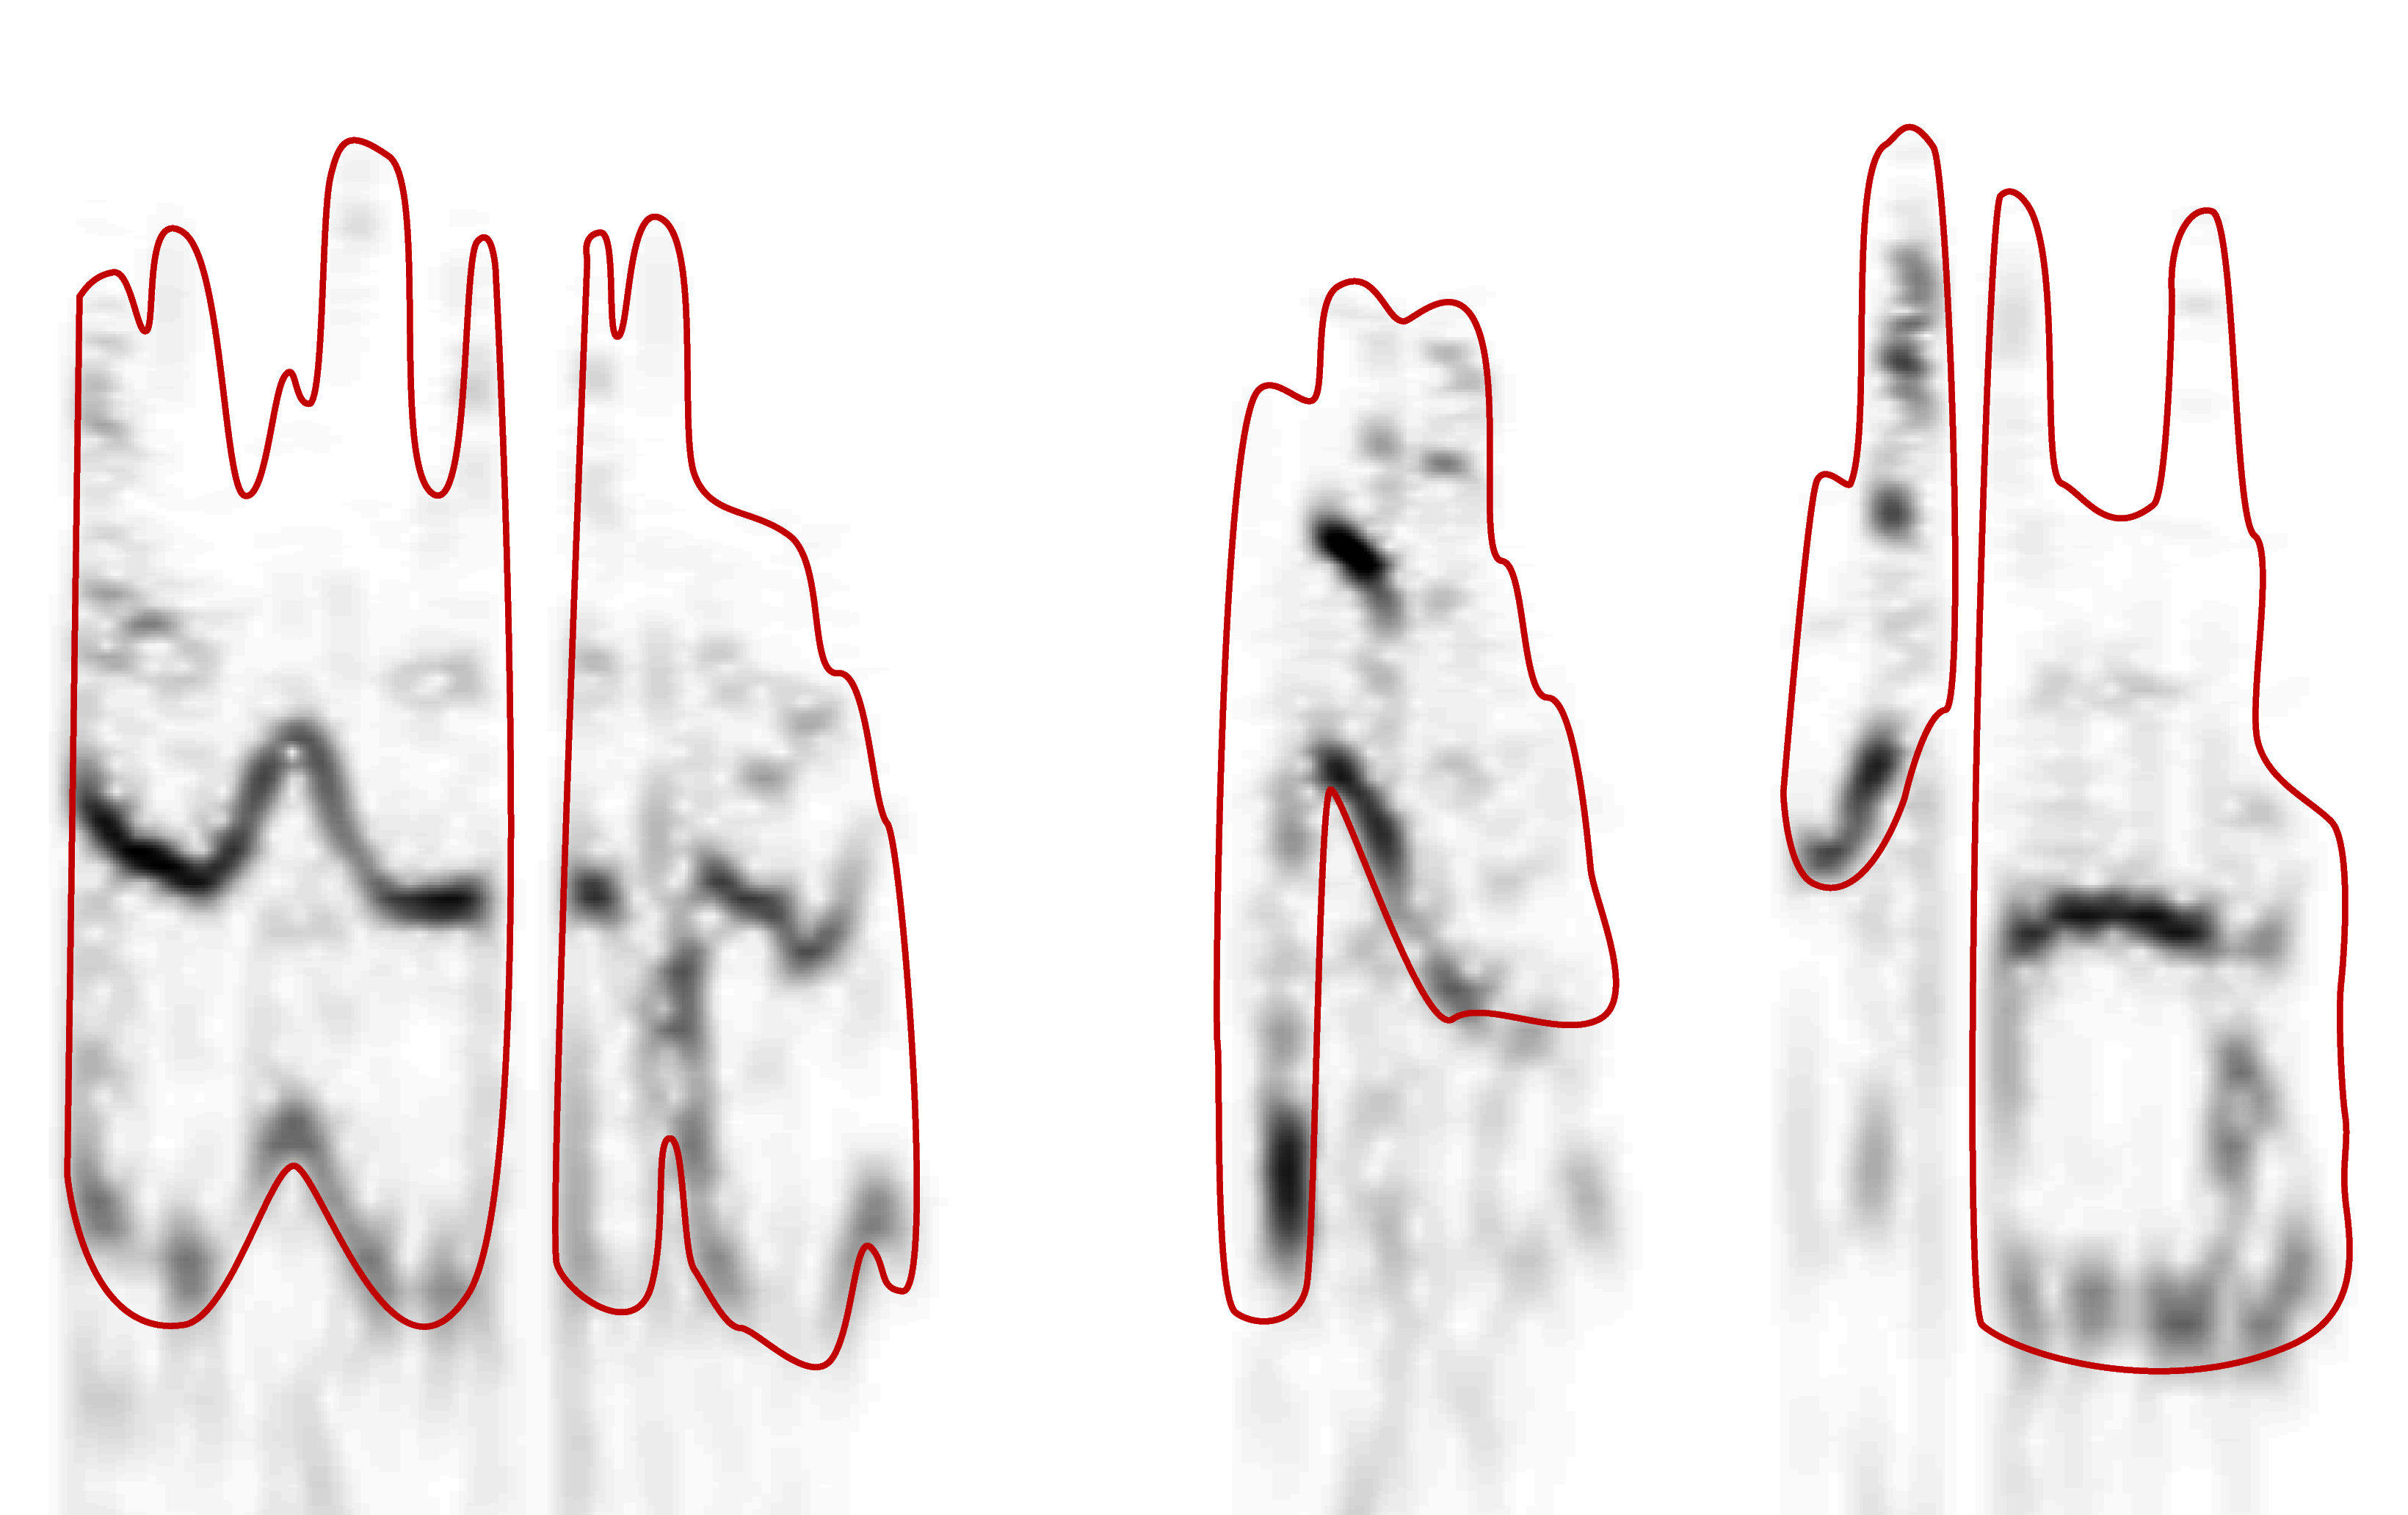
\includegraphics[width=10cm]{chapter5/spectovocal.tif} %change centimeters for resizeing
   \caption{FFTFilter: Spectral mapping of vocal contour.}
   \label{fig:example}
\end{figure}
shows a spectrogram of speech and how the FFTFilter maps the contour of the vocal signal. Given that the vocal signal has a strong presence in a narrow frequency range, it is ideal to control the filter. FFTFilter therefore uses the continuos signal of the highest and lowest frequencies of the array to calculate the bandwidth and center frequency for the resonant filter. Figure 5.2 shows a visual representation of a fairly noisy signal that has been filtered by the resonant filter following the vocal contour as seen in Figure 5.1. 
\begin{figure}[htbp] %  figure placement: here, top, bottom, or page
   \centering
   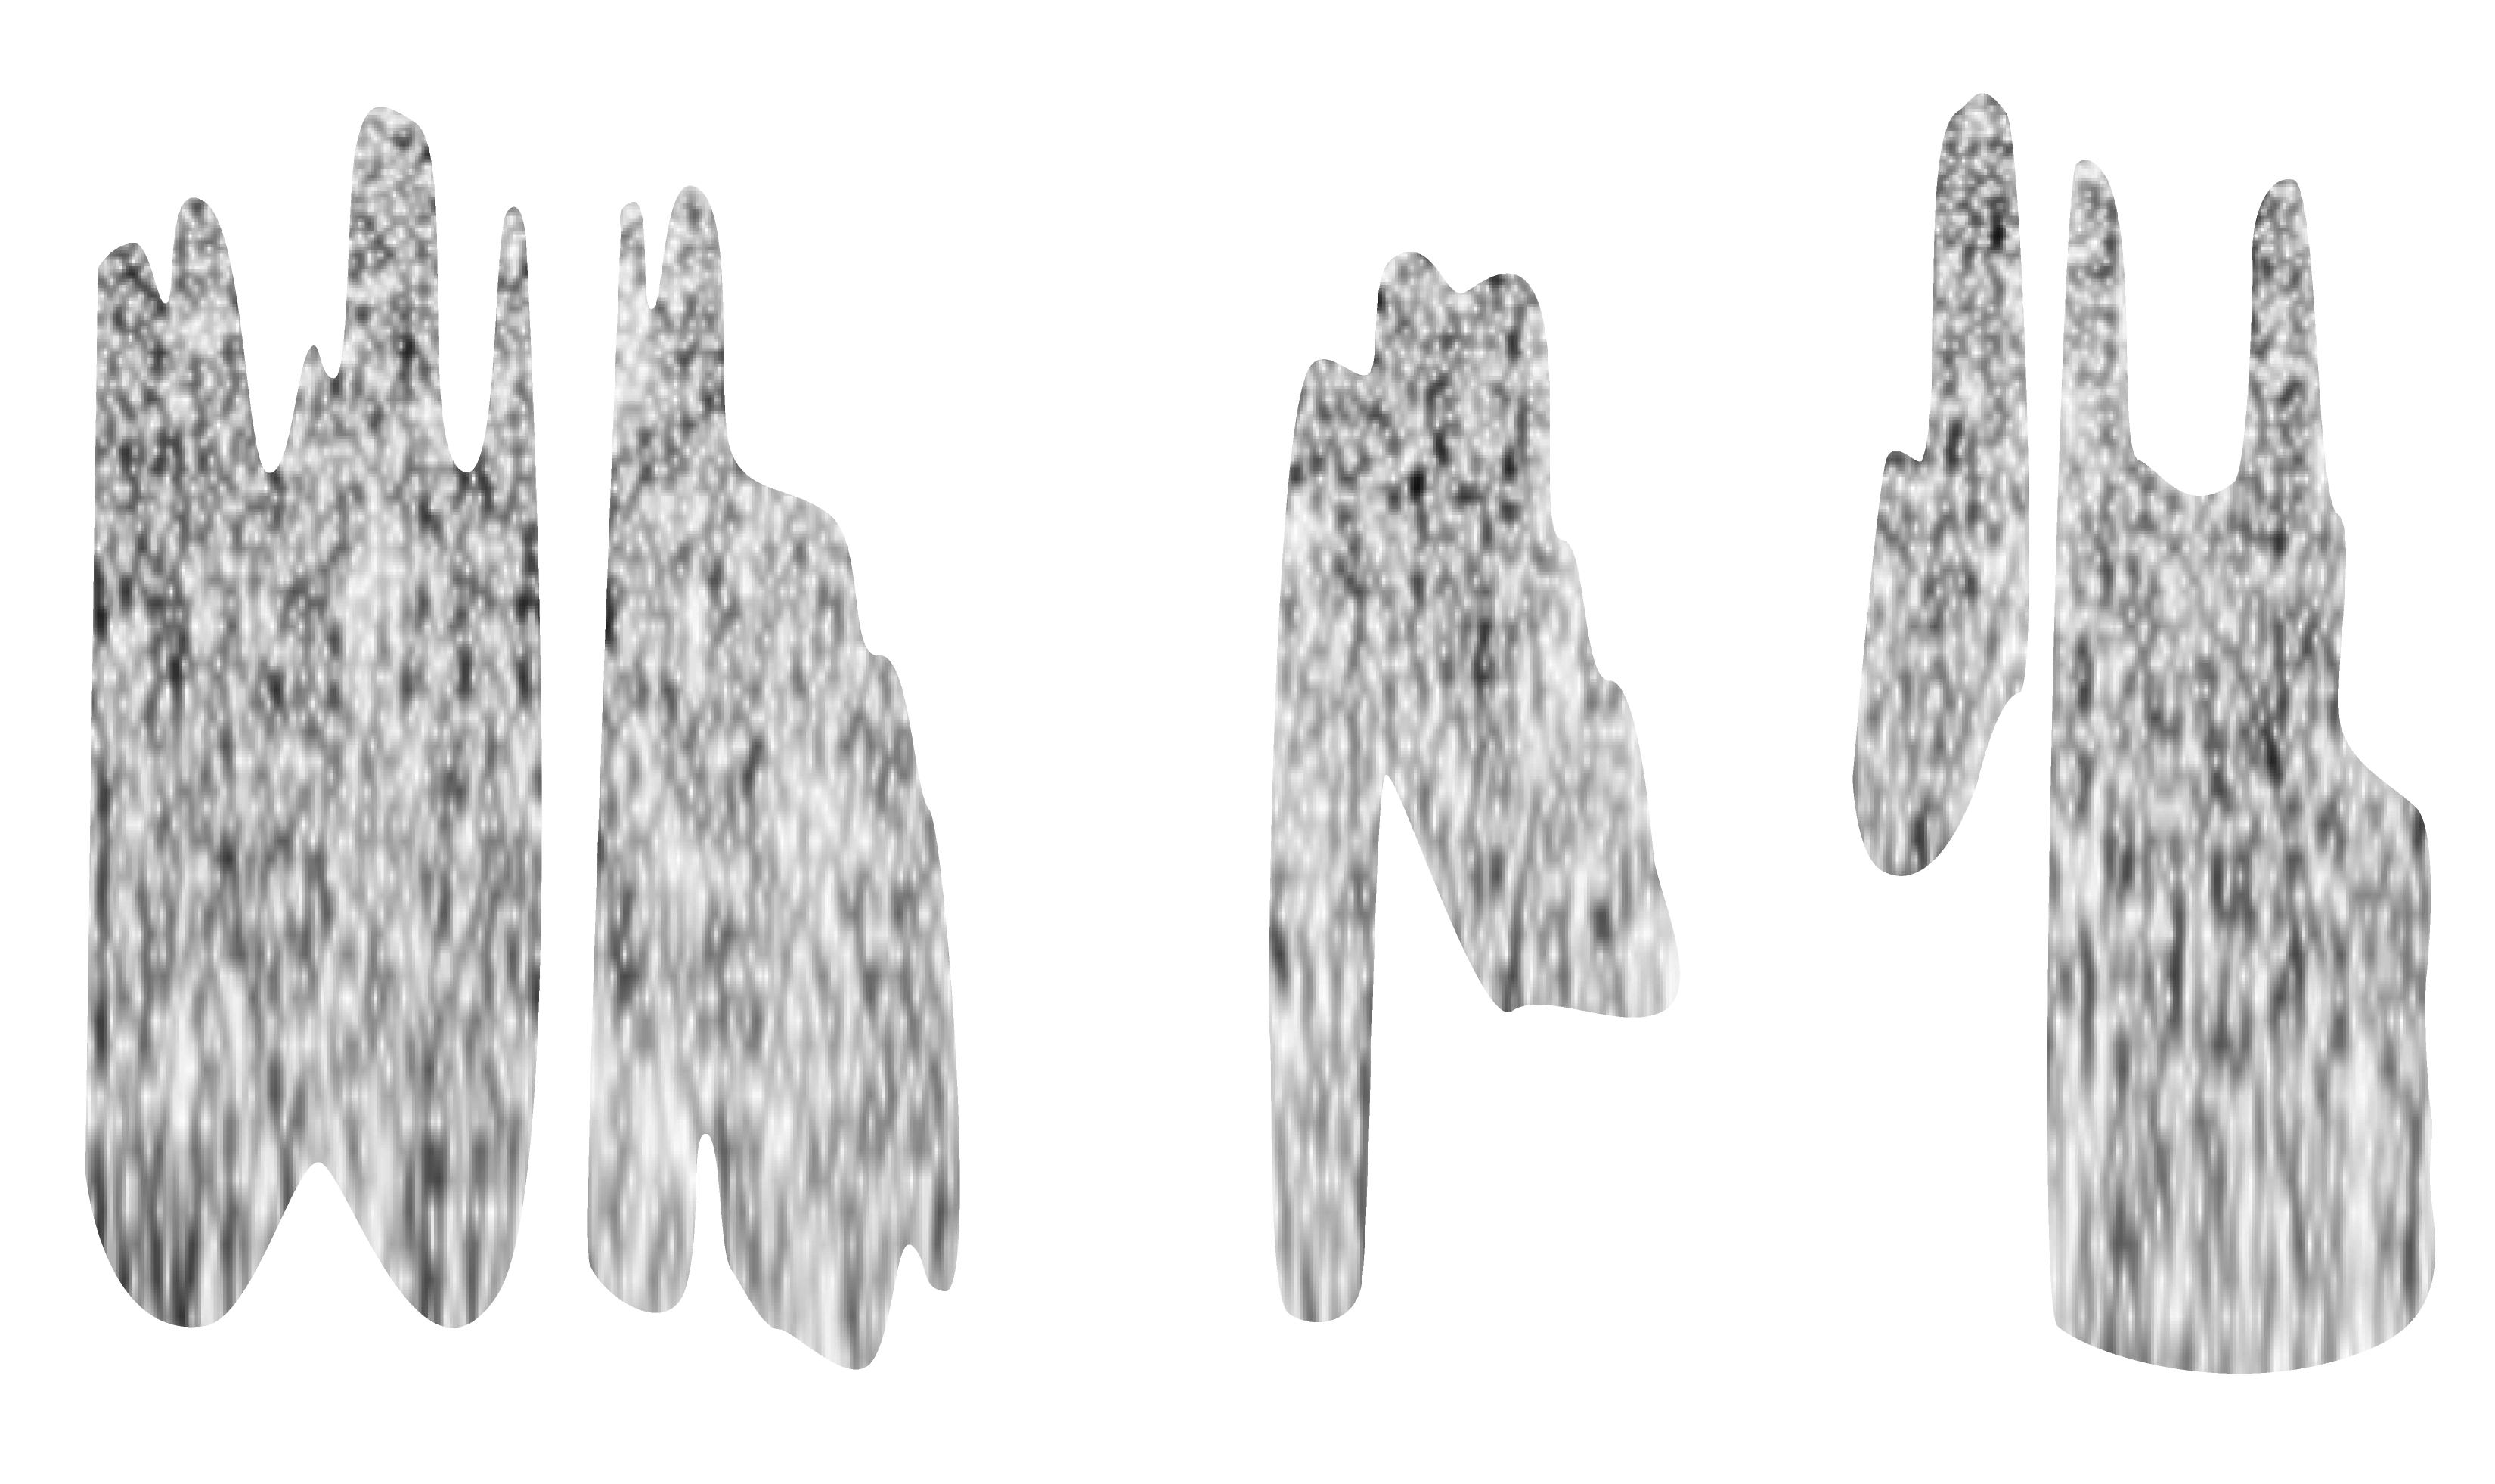
\includegraphics[width=10cm]{chapter5/spectonoise.tif} %change centimeters for resizeing
   \caption{FFTFilter: Noise filtered by vocal contour.}
   \label{fig:example}
\end{figure}
Ones the trajectory of the filter is set by the frequency data extracted from the FFT, an envelope follower maps the amplitude of the sound that was used as the FFT input to control the amplitude of the resonant filter. By combining the amplitude envelope and frequency contour of one sound to control a resonant filter that is applied to another sound, it is possible to incorporate characteristics of the analyzed sound to the filtered sound source.

\subsection{Spectral Data Extraction and Reduction}

The type of spectral information that can be extracted by using the SPEAR software can be useful as it could yield results that can be translated in valuable melodic and rhythmic material. For that reason I was attracted at the type of analysis that SPEAR performs. The advantage of SPEAR is that it allows to select each partial as a sinusoidal track from which we can more easily extract melodic content. In contrast to the PartialTracker class which takes the strongest bins at a given moment, SPEAR stores its information by partials and displays them visually so than one can select specific partials. Then one can access that information in a text file by partial instead of by frame, which facilitates the extraction of points within each partial. For that reason the data reduction in my opinion results in information can translate to gesture more successfully than for instance the PartialTracker class, or other form of partial extraction which attempts to derive chords either through a snapshot of an FFT or through the averaging of spectral data within an event determined by onset detection (an event being the time between the onsets). The drawback of this type of spectral extraction is that it can not be performed in real-time. I will therefore continue, by explaining how these classes take the data from SPEAR and reduces it to an amount of information that can be used for \emph{musica derivata}.

\hypertarget{spearsc}{}
\subsubsection{SpearToSC}

SpearToSC\footnote{See \href{http://github.com/freuben/FedeLib/blob/master/SpearToSC/SpearToSC.sc}{\texttt{http://github.com/freuben/FedeLib/blob/master/SpearToSC/SpearToSC.sc}}.} is a class that takes data from the open source software application called SPEAR\footnote{Klingbeil, Michael (2005), SPEAR, URL: \href{http://www.klingbeil.com/spear/}{\texttt{http://www.klingbeil.com/spear/}}.} and transfers it to an array in SuperCollider. SPEAR uses a variation of the traditional McAulay-Quartieri procedure to represent sounds as individual sine waves (for each partial) with time varying frequency and amplitude.\footnote{See \hyperlink{klingbeil}{Klingbeil (2005)}.} SPEAR provides a graphical representation of a sound\footnote{Spectral analysis, where the y-axis represents frequency in hertz and the x-axis represents time in seconds.} (as seen in Figure 5.3) in which it is possible to select the individual sinusoidal tracks and allows to isolate and access the information for each individual partial. 
\begin{figure}[htbp] %  figure placement: here, top, bottom, or page
   \centering
   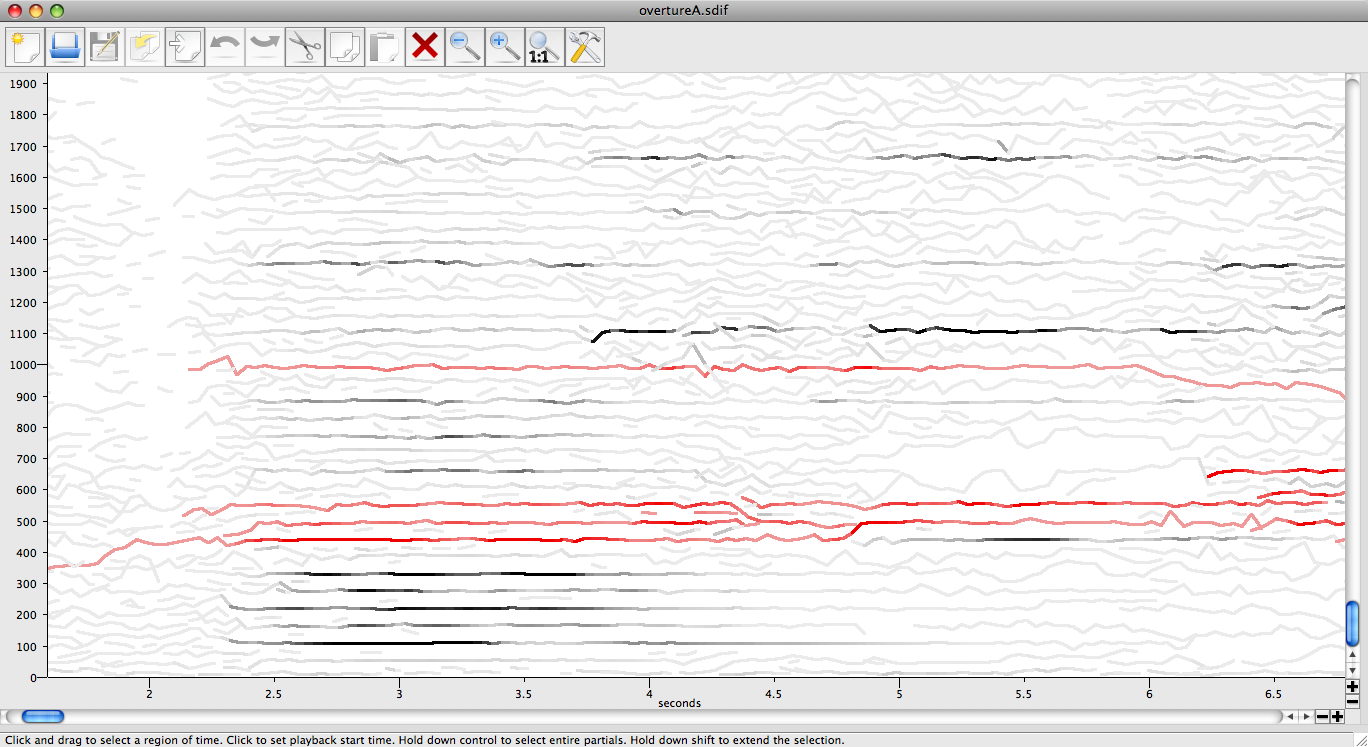
\includegraphics[width=15cm]{chapter5/Spear1.tif} %change centimeters for resizeing
   \caption{SPEAR graphical interface.}
   \label{fig:example}
\end{figure}
The amplitude and frequency information of each partial is given by frame and can be stored in a text file. SpearToSC reads the text file produced by SPEAR\footnote{SpearToSC reads SPEAR text files in the \emph{Text - Partials} format only.} as a string and strips it into a multidimensional array in SuperCollider. It is therefore possible to access and manipulate this data within the SuperCollider language and server and re-synthesize this information not only with sinusoidal waves, but with any type of unit generator. 

\subsubsection{SpearToMIDI}

SpearToMIDI\footnote{See \href{http://github.com/freuben/FedeLib/blob/master/SpearToSC/SpearToMIDI.sc}{\texttt{http://github.com/freuben/FedeLib/blob/master/SpearToSC/SpearToMIDI.sc}}.} is a class that inherits functionality from \hyperlink{spearsc}{SpearToSC} and reduces the information given by SPEAR to be used as data to produce a Midi file or to control SuperCollider synthesis definitions. The purpose of this class is to reduce the spectral information to an amount of data that can later produce notated material for a written score, a Midi file or a control system to be used for triggering synthesis algorithms. The data in the text file generated by SPEAR is available by frame and gives too much information for this purpose. Therefore, SpearToMIDI reduces this data in four stages: First, it takes a magnitude threshold argument which gets rid of all of the partial information that lies bellow this value (as seen in Figure 5.4).
\begin{figure}[htbp] %  figure placement: here, top, bottom, or page
   \centering
   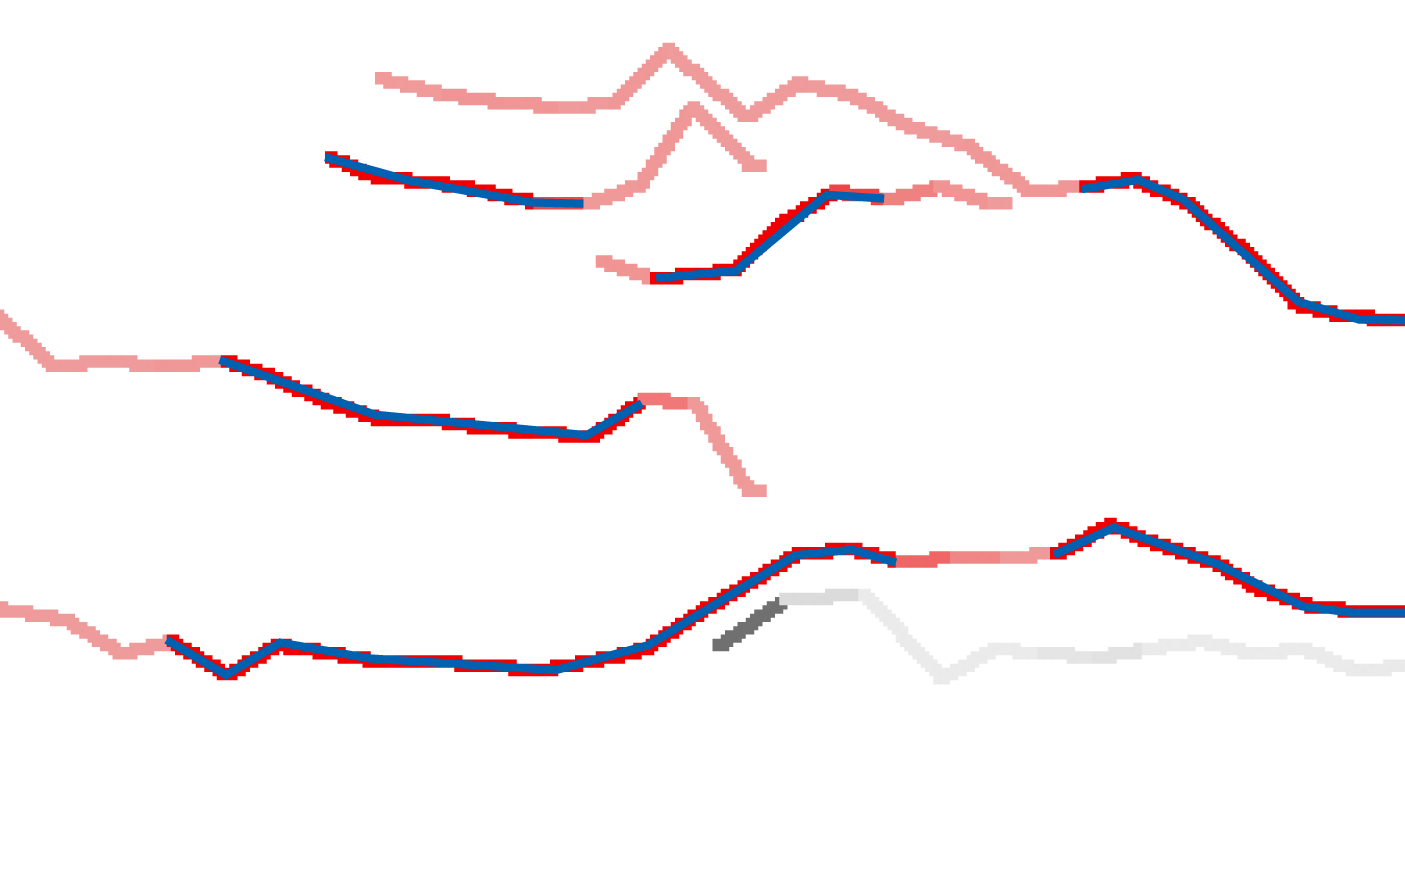
\includegraphics[width=9cm]{chapter5/Spear2.tif} %change centimeters for resizeing
   \caption{SpearToMIDI: Amplitude threshold selection.}
   \label{fig:example}
\end{figure}\
In other words, it breaks the partial in different groups by introducing silences instead of the data that lies bellow the threshold and at the same time keeps track of the beginning and the end of each group. 

The second stage reduces data with a frequency modulation threshold. Each group is taken as a line and the computer only stores the points in the line which cross a given interval (the modulation threshold). For example, Figure 5.5 shows how the lines representing the groups in Figure 5.4 are traced by selecting the points that cross a given interval.\footnote{The grid represents the intervals as shown in the y-axis. For the purpose of simplification, the diagram doesn't show a logarithmic representation of frequency.} 
\begin{figure}[htbp] %  figure placement: here, top, bottom, or page
   \centering
   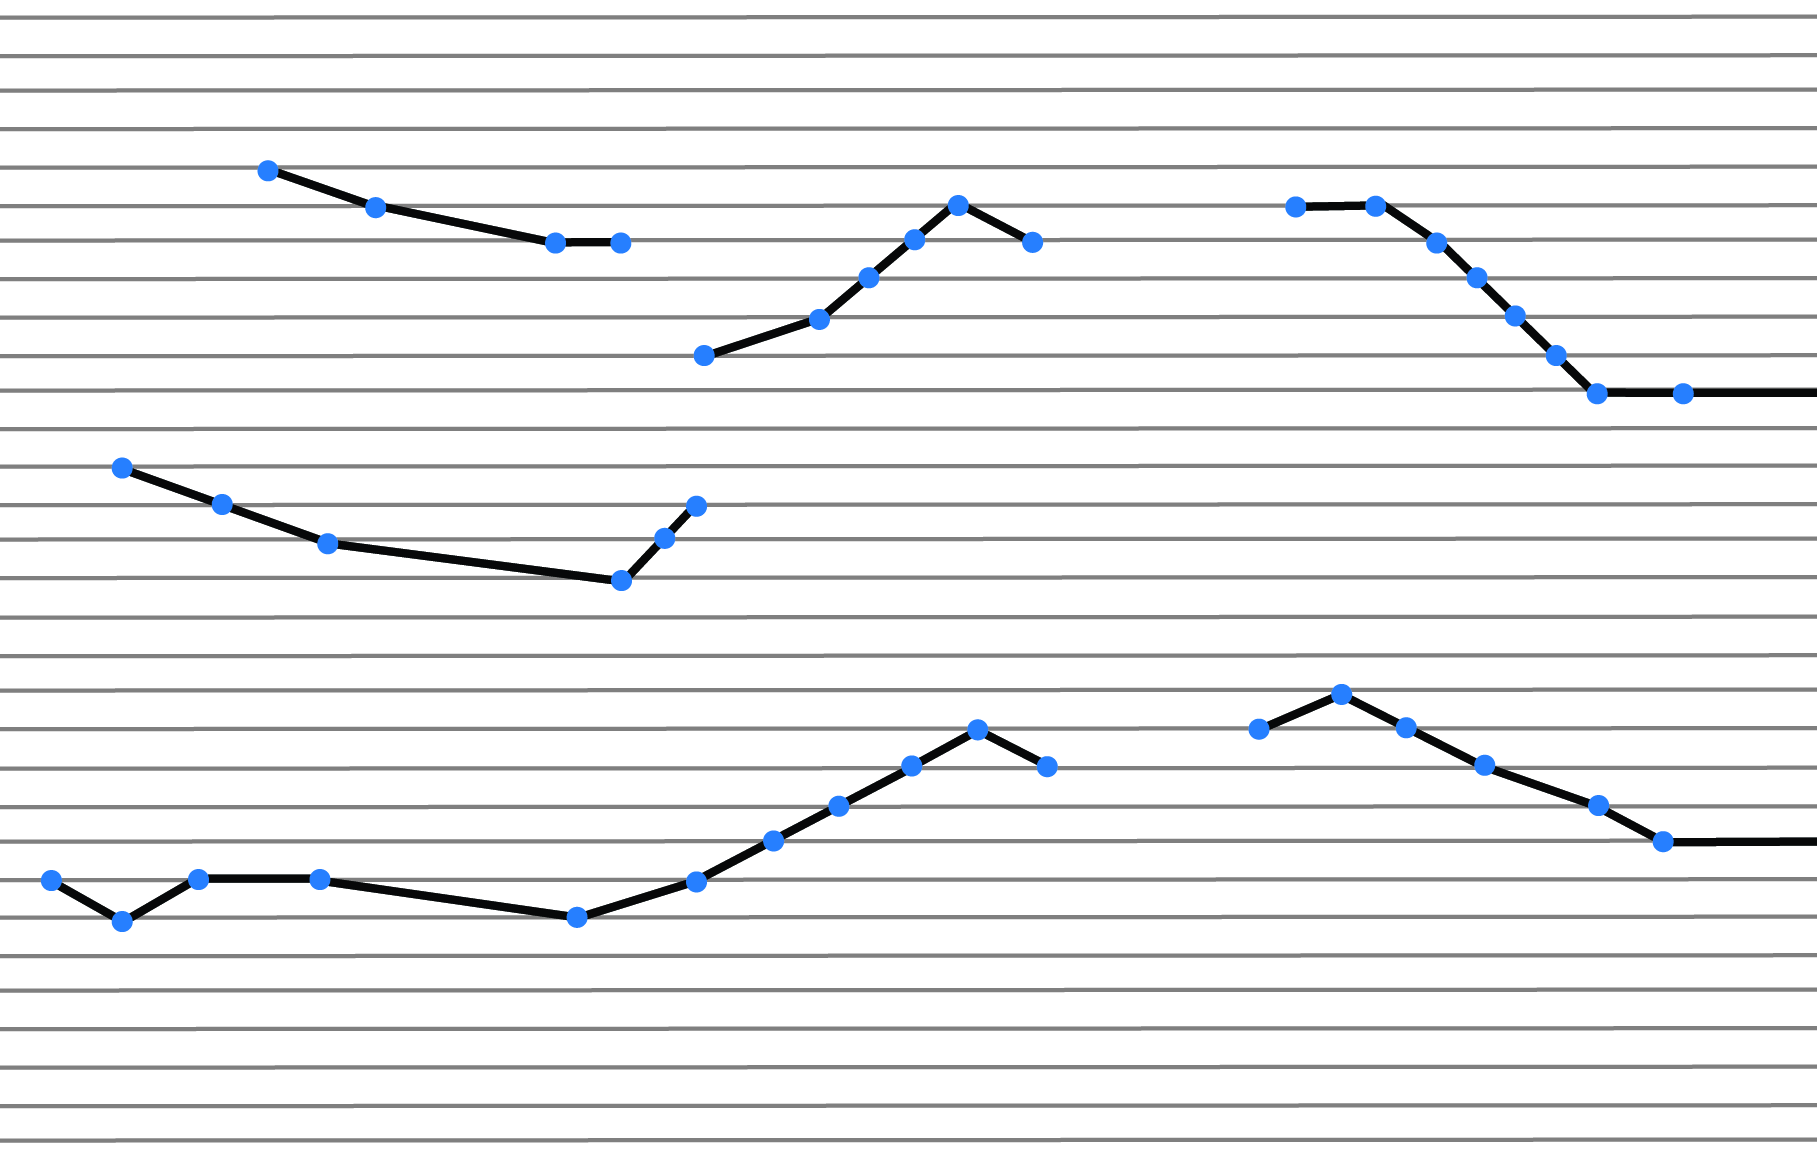
\includegraphics[width=10cm]{chapter5/Spear3.tif} %change centimeters for resizeing
   \caption{SPEARToMIDI: Point selection through frequency modulation threshold.}
   \label{fig:example}
\end{figure}\
If the interval is of one semitone then the frequencies are averaged to the closest chromatic note. It is possible to make microtonal divisions of the equal-tempered scale by using floating point values for the modulation threshold. The magnitude, frequency and time values of each point are stored as a collection of data. This collection can then be accessed and used to control synthesis definitions externally by generating envelopes, which gradually change frequency to produce glissandos and amplitude for gradual volume change. After these first two stages, the original data from Spear is reduced considerably by disregarding details that are not vital for the given purpose. 

The third stage, takes the points of the lines that were obtained in the previous stage and translates them into single notes with a start and an end and that do not change in frequency and amplitude while playing--- in other words, a format that is compatible with the Midi note-on and note-off paradigm. The points are then considered as representing note-on messages and the note-off messages are calculated depending on whether the point is followed by another new point or if the point is the last of the group, in which case a silence would proceed. In other words, a note-off is inserted before a new note-on or just before a silence. Figure 5.7 
\begin{figure}[htbp] %  figure placement: here, top, bottom, or page
   \centering
   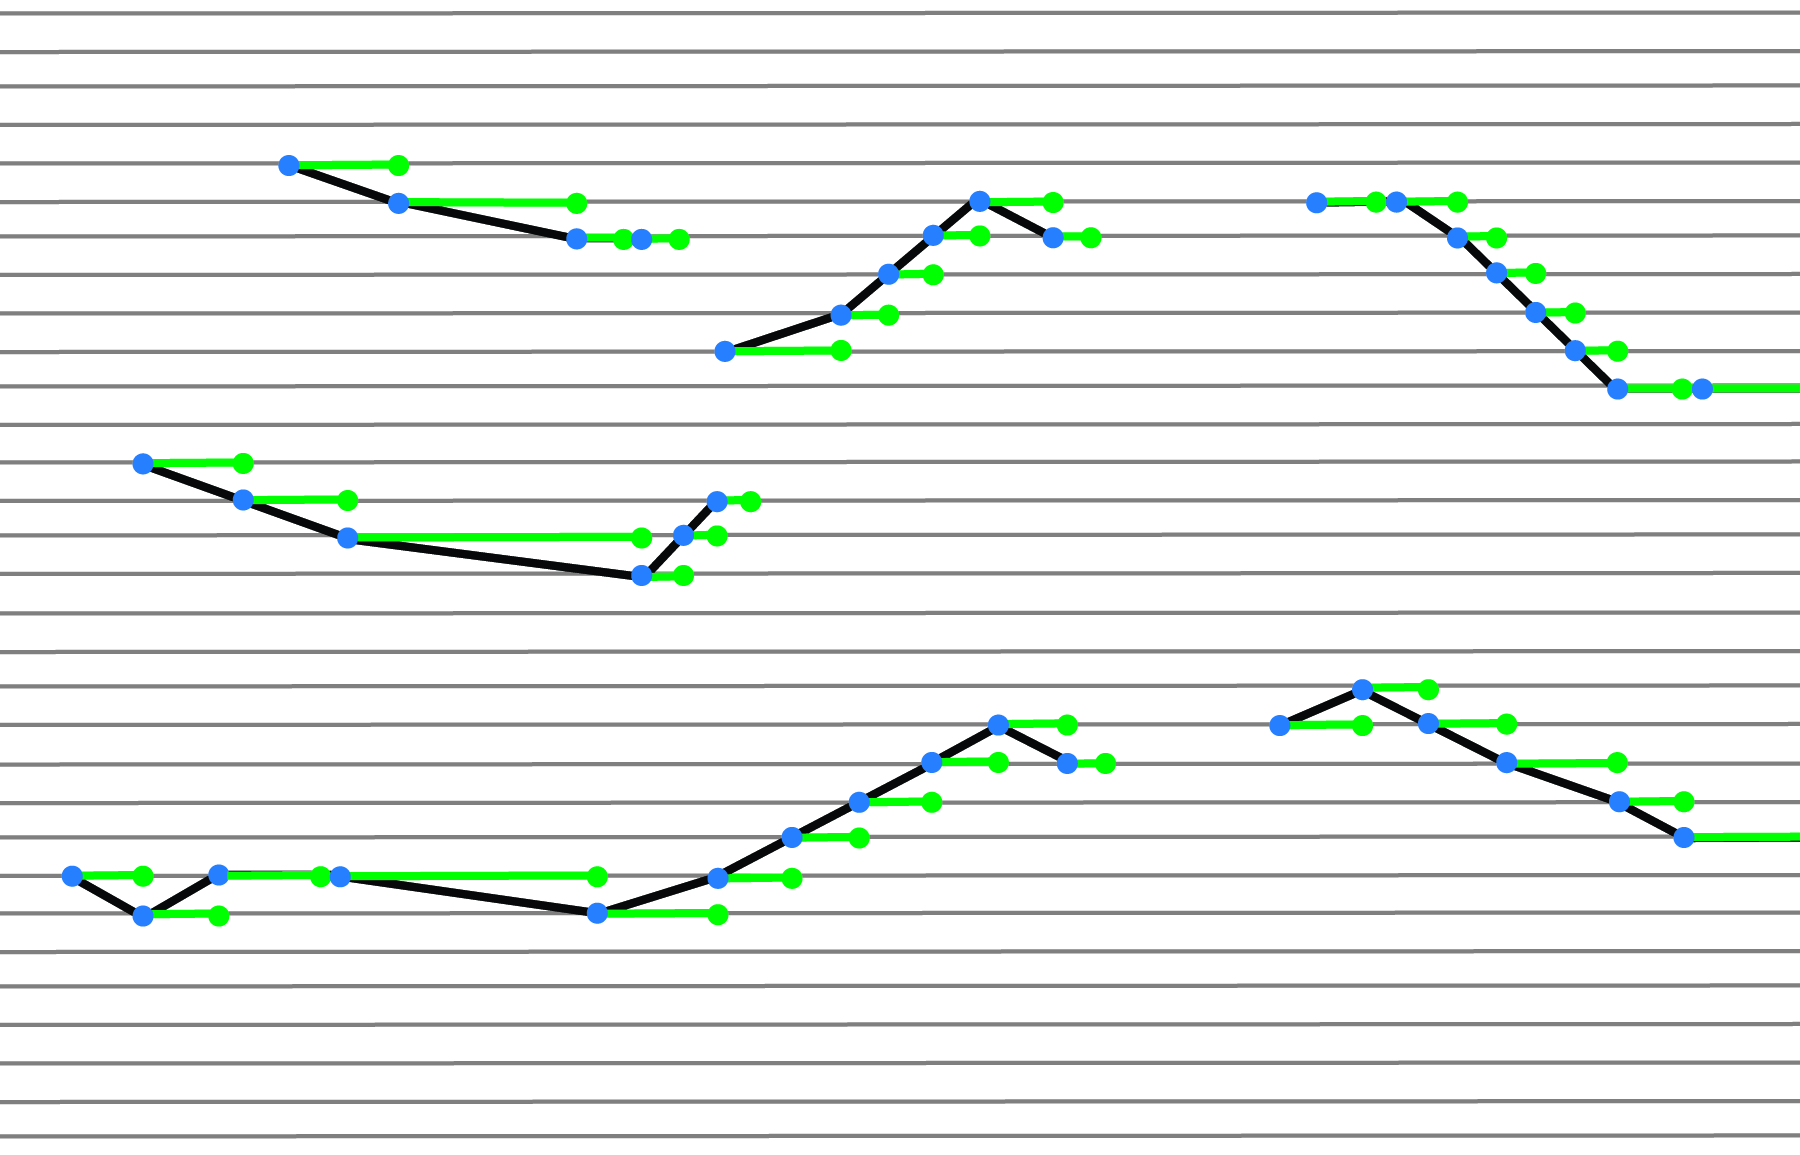
\includegraphics[width=10cm]{chapter5/Spear4.tif} %change centimeters for resizeing
   \caption{SPEARToMIDI: Note representation.}
   \label{fig:example}
\end{figure}\
shows the note representation derived from Figure 5.5, where the notes are seen as green lines, the note-on messages as blue points and the note off messages as green points. 
The results of this stage can be used to generate a Midi file\hypertarget{wlib}{}\footnote{Using the SimpleMIDIFile class that is part of wslib by \href{http://www.woutersnoei.nl/}{Wouter Snoei}, which is can be obtained as a Quark.} with the intention of either using it to trigger a sampler or to import it into a notation software to create a written score. The user can input the time signature and tempo for the Midi file as well as an interval value that divides the Midi note range into different Midi tracks. By doing this, the notes are separated into different tracks depending on their value in relationship to each other with the purpose of not having too many notes in the same track. Furthermore, these results can be used to create a list of Open Sound Control (OSC) commands that can be sent to the SuperCollider server for Real-Time-Synthesis and Non-Real-Time-Synthesis. Extra arguments can also be added to control other values in the synthesis definition, which can be set individually by using a function to be evaluated for each instance of the definition.

\section{Computer-Mediated-Performance}

In our discussion about \emph{interpassivity},\footnote{See \hyperlink{interpassiv}{pp. 48--52}.} I already pointed at some of the possibilities of using technology within a performance, not as an active agent which produces sound, but on the contrary as a passive agent which only gives instructions to the musicians on stage and directs them towards activity. The idea of using computer technology to direct performers rather than to produce sound inspired me to devise a series of computer-mediated-performance tools. The idea of implementing these tools was also attractive for the potential they show to rework musical strategies that have been established through conventions in composition and performance. Moreover, the idea to device such tools has also been largely motivated for the prospects they have to facilitate new collaborative possibilities with musicians that come from different performance backgrounds and traditions. During the research period, I have put into practice these performance tools with musicians from a diverse background---some trained as classical performers who read notation and some as improvisers---yielding very positive results that can be found in the submitted work.

\subsection{Real-Time Scoring}

The most important aspect of the computer-mediated-performance tools I have developed is their real-time scoring capabilities. The main motivation behind writing this computer score with real-time capabilities was Simon Emmerson's idea of creating a `superscore' that combines visual and oral forms communication within a multimedia object.\footnote{See \hyperlink{superscore}{pp. 41--44}, for a further discussion about Emmerson's `superscore' and some ideas of how to develop it'.} When I had in mind implementing such a computer programme, I decided that it would have to be flexible enough to use different types of notation and graphics, it would have to display conventional and colored text as well as images and videos. The programme also would have to have the ability to display visually the results from algorithmic/generative process and from real-time audio analysis. Nevertheless, the most important consideration was that it had to be dynamic and be able to not only direct the performers on stage through time structures but also to generate score animations. The aural part of the score would not only have to be synchronized with the visual element, but would be able to be generative.\footnote{The results of the computer-score I devised can be appreciated in \emph{On Violence} and \emph{\v{Z}i\v{z}ek!?}. See DVD II and III.} Given all of the complications that building a standalone application that would perform all of the above-mentioned functions implied and that I wanted to keep the application flexible enough, I decided to instead implement it as separate SuperCollider classes that one could integrate as one wished. Therefore, the audio and the visual elements, even though they can be synchronized, are run through separate classes. Given that SuperCollider is a computer language that specializes in audio and has already many implemented functionalities that I could use for the aural elements of the score, the crucial element I attempted to implement was the visual features. This resulted in a SuperCollider class which is flexible enough to convey different types of notation, graphics and directions as well as adding movement to the expressive palette of a conventional paper score. I will therefore continue by describing how these class was implemented and how it works.

\subsubsection{AlgorithmicScore}

AlgorithmicScore\footnote{See \href{http://github.com/freuben/FedeLib/blob/master/AlgorithmicScore/AlgorithmicScore.sc} {\texttt{http://github.com/freuben/FedeLib/blob/master/AlgorithmicScore/AlgorithmicScore.sc}}.} is a class that visualizes different types of notation in real-time. It is programmed as a graphical user interface (GUI) in SuperCollider but receives no input in the GUI window itself. Instead, this class only displays notes, letters, symbols and other visual aids for real-time scoring from code that can be evaluated in the interpreter, or within a compiled class in the SuperCollider language. It displays traditional musical symbols including notes, accidentals, clefs and dynamics that are available as fonts\footnote{The fonts I used for the AlgorithmicScore class are MusiSync by Robert Allgeyer and Sonora by Christian Texier.} in combination with non-standard notations. Stems and flags are purposely not implemented so that too much visual information is not given to the performer while following the score. Note-heads can be of different type and color. There are four types of different clefs that are implemented: treble, bass, alto, tenor.  If a clef is selected, a staff is generated in which the notes will appear. The information to be placed in the score can be evaluated in an array consisting of the note position from left to right, staff number, note-head type, note, accidental and color. There are three array types that can be used which respond to different notation modes: free, enharmonic and chromatic. In the free mode, notes are selected by a number that does not correspond to the clef but to the position from top to bottom starting with zero as the first leisure line bellow the bottom line of the staff. Moreover, the note value can not only be negative but also a float number, which results in a position in between notes. This mode can be useful for conveying movement if the score were to be animated. The enharmonic mode, takes a string representing the note and octave---were c4 equals middle C---and positions the note according to the selected clef. It is also possible to select the type of accidental between flat, sharp and natural. If the note exceeds four leisure lines, the programme places an \emph{8va} sign and if it is exceed it by yet another octave, it places a \emph{15ma} sign. The chromatic mode, is similar to the enharmonic, but only uses sharps as accidentals and places a natural in front of each note that is diatonic. This mode is useful to receive note information as Midi numbers. In addition, it is possible to place written directions with different colors in the score.

The following code example produces a score in real-time if evaluated from the interpreter window: 
\begin{verbatim}
a = AlgorithmicScore.screenBounds; //start class
a.score([\bass, \treble, \treble]); //3 staffs
//[pos, [staff, noteType, note, acc, color]]:
~staff1 = [[0, [0, 1, "c3"]], [1, [0, 0, "b3", \flat, \blue]]]; 
~staff2 = [[0, [1, 0, "d5", \flat]]];
~staff3 = [[0, [2, 1, "a3", \nat, \red]]];
a.enharmonic(~staff1 ++ ~staff2 ++ ~staff3); //writes notes
a.expression("p"); //expression for dynamics
a.text("Improvise with pitch material", "Helvetica", 30, 30, 200, color: Color.rand);
//string, fontType, letterSize, inLeft, inTop, color  
\end{verbatim}
The code generates a new window and three staffs with one bass and two treble clefs. The separate arrays correspond to each staff\footnote{Note that the first value is for the position of the note from left to right and that the values are already scaled so that in the entire length of screen can fit 24 notes.} and are concatenated to respond to the enharmonic mode. In addition, an expression to play \emph{piano} and a text description are added. Figure 5.7 shows the GUI that the AlgorithmicScore class creates when the code above is evaluated. 
\begin{figure}[htbp] %  figure placement: here, top, bottom, or page
   \centering
   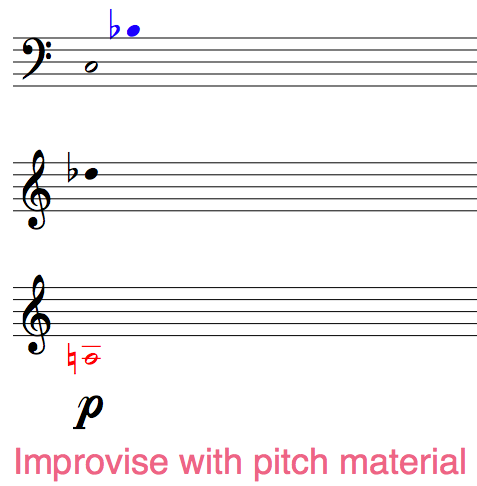
\includegraphics[width=9cm]{chapter5/algoscore1.tif} %change centimeters for resizeing
   \caption{AlgorithmicScore: Enharmonic mode.}
   \label{fig:example}
\end{figure}\

Another feature of the application is a piano clef type which instead of creating only one staff that responds to the corresponding clef, it produces two staffs with one treble clef on the top staff and one bass clef on the bottom staff. In this clef type, the note is placed on the treble clef staff if it is higher or equal to middle C and if it is lower than middle C, it is placed on the bass clef staff. Furthermore, it is possible to score in real-time by evaluating an array of Midi note numbers. The class takes the Midi numbers and translates them to the correct pitch type and octave in the chromatic mode. This procedure is a very convenient form of sending Midi values to be scored in real time. The following example of code takes sixteen random notes from f1 to g6 and chooses one of them randomly and changes its color to red:
\begin{verbatim}
a = AlgorithmicScore.screenBounds; //start class
a.score([\piano]); //piano staff
~notes = Array.fill(16, {rrand("f1".notemidi,"g6".notemidi)}); 
//random notes between f1 and g6
~color = Array.fill(~notes.size, \black).insert(rrand(0,15),\red);
//all notes black, except a random red note
a.notes(~notes, color: ~color);
\end{verbatim}
\begin{figure}[htbp] %  figure placement: here, top, bottom, or page
   \centering
   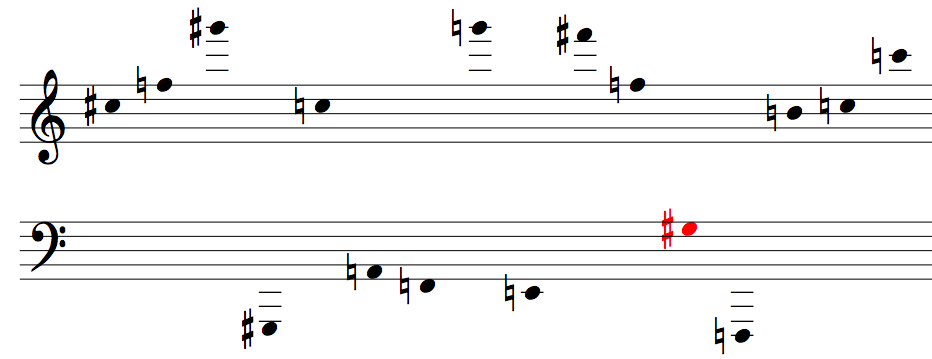
\includegraphics[width=14cm]{chapter5/algoscore2.tif} %change centimeters for resizeing
   \caption{AlgorithmicScore: Chromatic mode.}
   \label{fig:example}
\end{figure}\
The \emph{notes} message\footnote{A message is the type of operation that the class performs depending on the type of message it receives.} takes as input one array of notes, one of positions and one of colors. If the array of positions is not specified, the computer arranges the positions equally from left to right. Figure 5.8 shows the resulting score generated by the code. Note that the notes are spread between the treble and bass clefs because the piano clef type is selected. 

This method for generating scores can be very useful to notate pre-composed and aleatoric material in real-time. Moreover, this application is ideal to to visualize pitch or rhythmic information derived from machine listening techniques such as partial tracking. Real-time scoring is especially relevant when using machine listening applications because the material that is notated is extracted from sound characteristics that are specific to the moment and space of the performance. \mbox{Figure 5.9} shows an example that uses the \hyperlink{partrack}{PartialTracker} class to extract Midi note numbers from the strongest twenty partials of a spectrum. The resulting score is therefore generated in real-time and is specific to the space and time in which the partials are extracted.
\begin{figure}[htbp] %  figure placement: here, top, bottom, or page
   \centering
   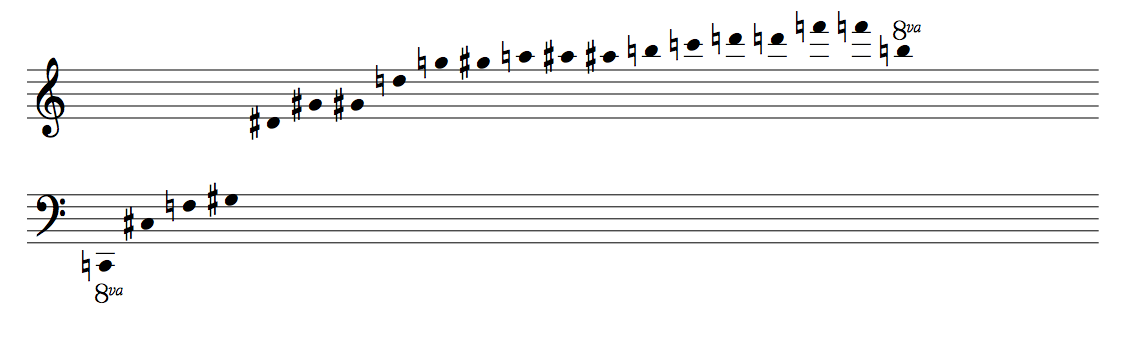
\includegraphics[width=17cm]{chapter5/algoScore_partials.tif} %change centimeters for resizeing
   \caption{AlgorithmicScore: PartialTracker to Notes.}
   \label{fig:example}
\end{figure}\

A sense of movement can be generated using the AlgorithmicScore class if the notes and other graphics are imbedded within a \emph{routine}.\footnote{Routines in SuperCollider are functions used for scheduling timed events using a clock that can be specified.} Therefore, it is possible to animate the graphical user interface including the notation elements for different purposes. One purpose for using score animations is to convey a sense of gesture by animating the notes so that they appear to be moving in specific directions. It is possible then to make notes appear as if they are skipping or jumping by changing note values every time an element of the \emph{routine} is evaluated.\footnote{For example, see DVD III (\emph{\v{Z}i\v{z}ek!?}) \tiny \textgreater \footnotesize \hspace{0pt} Documentation \tiny \textgreater \footnotesize \hspace{0pt} Performance Materials \tiny \textgreater \footnotesize \hspace{0pt} Score Parts \tiny \textgreater \footnotesize \hspace{0pt} Piano \tiny \textgreater \footnotesize \hspace{0pt}\mbox{\emph{12:30--13:05}}.} It is also possible to achieve a sense of a note gradually moving horizontally by gradually changing the numbers for the position of a note. In addition, one can animate the direction vertically by gradually changing the note values in free mode.\footnote{See DVD III (\emph{\v{Z}i\v{z}ek!?}) \tiny \textgreater \footnotesize \hspace{0pt} Documentation \tiny \textgreater \footnotesize \hspace{0pt} Performance Materials \tiny \textgreater \footnotesize \hspace{0pt} Score Parts \tiny \textgreater \footnotesize \hspace{0pt} Bass \tiny \textgreater \footnotesize \hspace{0pt} \mbox{\emph{12:35--13:15}}, for an example of notes gradually moving horizontally and vertically.} Furthermore, generating movement in real-time scoring can express timing and other conducting cues and gestures. The AlgorithmicScore class gives the possibility of scheduling a mixture of written directions, notation, chronometers, arrows and other graphics.  Visual cues can be given through the computer display to signal the beginning and end of sections as well as other important timing instructions. The use of colors to indicate silence and new sections is also possible when using this class.\footnote{See DVD III (\emph{\v{Z}i\v{z}ek!?}) \tiny \textgreater \footnotesize \hspace{0pt} Documentation \tiny \textgreater \footnotesize \hspace{0pt} Score Demo, for an example of this applications of real-time scoring.} 

Given that the AlgorithmicScore class does not use note stems and flags as an element of notation, rhythm may be expressed visually as well as aurally. Rhythm might be expressed with score movement using visual triggers that turn \emph{on} and \emph{off} symbolizing the onset and release of a note---this class has circular triggers that switch between bright colors (\emph{on}) and light grey (\emph{off}) to convey rhythm.\footnote{For example, see DVD III (\emph{\v{Z}i\v{z}ek!?}) \tiny \textgreater \footnotesize \hspace{0pt} Documentation \tiny \textgreater \footnotesize \hspace{0pt} Performance Materials \tiny \textgreater \footnotesize \hspace{0pt} Score Parts \tiny \textgreater \footnotesize \hspace{0pt} Drums \tiny \textgreater \footnotesize \hspace{0pt} \mbox{\emph{12:25--13:00}}.} Another strategy to express rhythm through score movement is by changing the color of only one note at a time within a sequence of notes---the logical movement being from left to right.\footnote{For example, see DVD II (\emph{On Violence}) \tiny \textgreater \footnotesize \hspace{0pt} Documentation \tiny \textgreater \footnotesize \hspace{0pt} Performance Materials \tiny \textgreater \footnotesize \hspace{0pt} Score Demo \tiny \textgreater \footnotesize  \hspace{0pt} \mbox{\emph{4:25--7:00}}.} Aural triggers may be added to indicate both rhythm and pitch by producing sounds that will serve as guide to the performer. The sounds would account for an aural score that the performer would receive through headphones and might enhance the visual elements of the AlgorithmicScore class.

Additionally, it is possible to import any type of image and video within the class and therefore create a wide variety of non-standard graphical indications. This application also provides the option to import scores written traditionally in standard notation programmes and combine them with the more expressive potential of the AlgorithmicScore class. Finally, by using human interface devises (HIDs) such as Midi controllers and pedals the performer may interact with the score. This might be helpful for example to trigger score animations or turn pages with a Midi pedal. Other examples of human-to-score interaction include controlling tempo and conducting cues with human gesture and triggering spectral data extraction to be displayed in the computer display with different types of sensors. 

\section{Computer-Aided-Composition Tools}

As part of my creative output, I have developed computer applications that served me as computer-aided-composition (CAC) tools during my research. This set of tools can be found in a library of  SuperCollider classes and extensions called FedeLib.\footnote{See \href{http://github.com/freuben/FedeLib}{\texttt{http://github.com/freuben/FedeLib}}.} An important component to this library is a collection of extensions\footnote{These extensions can be found at \href{http://github.com/freuben/FedeLib/tree/master/Extensions/}{\texttt{http://github.com/freuben/FedeLib/tree/master/Extensions/}}.} to existing classes that perform a wide variety of tasks. These tasks include: mathematical operations on simple numbers and lists; musical calculations including different types of tuning systems, interval and pitch-class recognition, scale generation and voice leading; scheduling and time related applications; operations on strings; envelope generation; recurrent operations such as recording audio, handling Midi, switching between servers, managing buffers and patterns; Midi file analysis, transformation and triggering; and GUI creation. These tools aided me in the composition of the works submitted and might be useful to other composers. They too might reflect some of my compositional interests and methods. Nevertheless, I will not attempt to describe all extensions as it would be out of the scope of this discussion. Therefore, I will focus only on a few tools that I think are fundamental in my creative process as they are related with the concepts described in the previous chapters.

\subsection{Score Visualization}

During several years, I have developed pre-compositional tools that help me organize my music and think in terms of structure at different levels of abstraction. I normally start a piece of music with an idea of a macro-structure and then gradually start considering the micro-elements of the composition. That is to say, usually I first establish a foundation or blueprint that determines the structural decisions of a composition before I start working on the details that are related to smaller temporal intervals. As I became interested in deriving elements of existing compositions in my work, I decided to abstract other pieces of music by other composers that I consider excel in dealing with macro-structure.\footnote{In the discussion about musical appropriation, I have already discussed the possibilities of appropriating only \emph{macro} elements of already existing music. See \hyperlink{macroplunder}{pp. 91--92}.} Therefore, I started by analyzing the score of these compositions and then tracing their phrase structure that I would use as a blueprint for my own composition. Each voice or staff would be considered as different layers containing phrases that would start and end depending on where silences occur. I would then create `empty containers'\footnote{This is a concept originally formulated by John Cage. See \hyperlink{landscape5}{p. 84}.} with the phrase structure of each voice of the appropriated composition. Consequently, I would sketch in a piece of squared paper the start and end of phrases according to a time scale. Ones I would sketch a diagram of ``empty containers'', I would start thinking what sonic `material' I would fill the containers with and how this `material' would develop. Normally, I would also treat this `material' by processing it with information derived from the melodic contour of the original phrases and relating it to the harmonic elements of the original composition. As I become more experienced as a composer, I adhere less to this idea of thinking of music as controlled layers of sound or music and take less rigid interpretation of these blueprints. Nevertheless, I still always begin by reducing an existing score by another composer to its basic marco-elements as a starting point for my own composition. 

Considering that this is a process that is recurrent in my compositional practice and I always sketch the phrase structure of the existing scores similarly on paper, I decided to programme an application in SuperCollider that takes information from a Midi file and creates a visualization of its phrase structure. Therefore, I developed extensions for the SimpleMIDIFile\footnote{SimpleMIDIFile accesses Midi file information in SuperCollider. See footnote number \hyperlink{wlib}{14}.} class to perform these operations. The message \emph{trackSilence}\footnote{See \href{http://github.com/freuben/FedeLib/blob/master/Extensions/FedeExtensions.sc}{\texttt{http://github.com/freuben/FedeLib/blob/master/Extensions/FedeExtensions.sc}.} for the FedeLib extensions including SimpleMIDIFile's \emph{trackSilence} message.} analyses a Midi file\footnote{The Midi file's content must have the standard Midi layout and specifications for scored music. If a Midi file does not follow this specifications, it can be edited so that it meets the requirements for a coherent visualization.} track and locates the starting and ending points of silences. The application analyses the Midi note-on and note-off messages and finds the moments where notes are not being played. It is possible to specify a time threshold (either in ticks or seconds) that ignores silences smaller than the given value. This way silences that are shorter than those which are notated may be ignored such that only the written silences are considered. The following example shows  the results given in a multidimensional array that specifies the start and end times of the silences.
\begin{verbatim}
[ [ 17.14284, 17.92206 ], [ 38.961, 40.51944 ], [ 50.416336, 51.034892 ], 
[ 56.601896, 57.220452 ], [ 70.210128, 72.065796 ], [ 88.77462, 89.154366 ], 
[ 95.610048, 96.36954 ], [ 105.483444, 106.242936 ], [ 118.394808, 119.1543 ] ]
\end{verbatim}

Ones the results for the timings of silences for each track of the Midi file are obtained, it is possible to create a visualization of the phrase structures. The \emph{phraseStructure} message creates a GUI window that displays this information by converting time values to pixels to create a visual representation of the Midi file. Figure 5.10 shows the result of the visualization of a Midi file of a section of Johannes Ockeghem's \emph{Missa Mi mi}. 
\begin{figure}[htbp] %  figure placement: here, top, bottom, or page
   \centering
   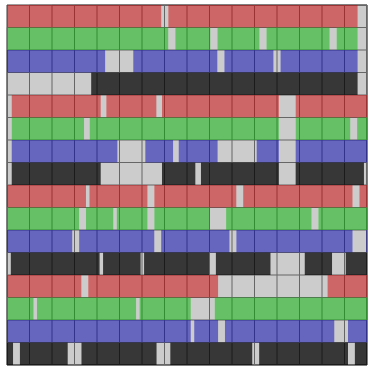
\includegraphics[width=8cm]{chapter5/midi_phrase.tif} %change centimeters for resizeing
   \caption{Visualization of Ockeghem's \emph{Missa Mi mi}.}
   \label{fig:example}
\end{figure}\
Each Midi track is represented as a different color and the silences are displayed in light grey. The Midi tracks represent the different voices of the \emph{Missa Mi mi}, where the red stands for the \emph{discantus}, the green for the \emph{contratenor}, the blue for the \emph{tenor} and the black for the \emph{bassus}. The x-axis represents time and each square equals to a value for time that can be specified by the user. This enables the user to `zoom' in and out of the phrase structure. The combinations of this elements of representation result in a visualization of the phrase structure for each voice of the existing composition that may serve as a map of the structure or blueprint for the new work. The application can also produce a black and white printable version of the visualization. Figure 5.11 shows a printable version of the visualization of the Midi file of Gesualdo's madrigal \emph{Se la mia morte brami}. 
\begin{figure}[htbp] %  figure placement: here, top, bottom, or page
   \centering
   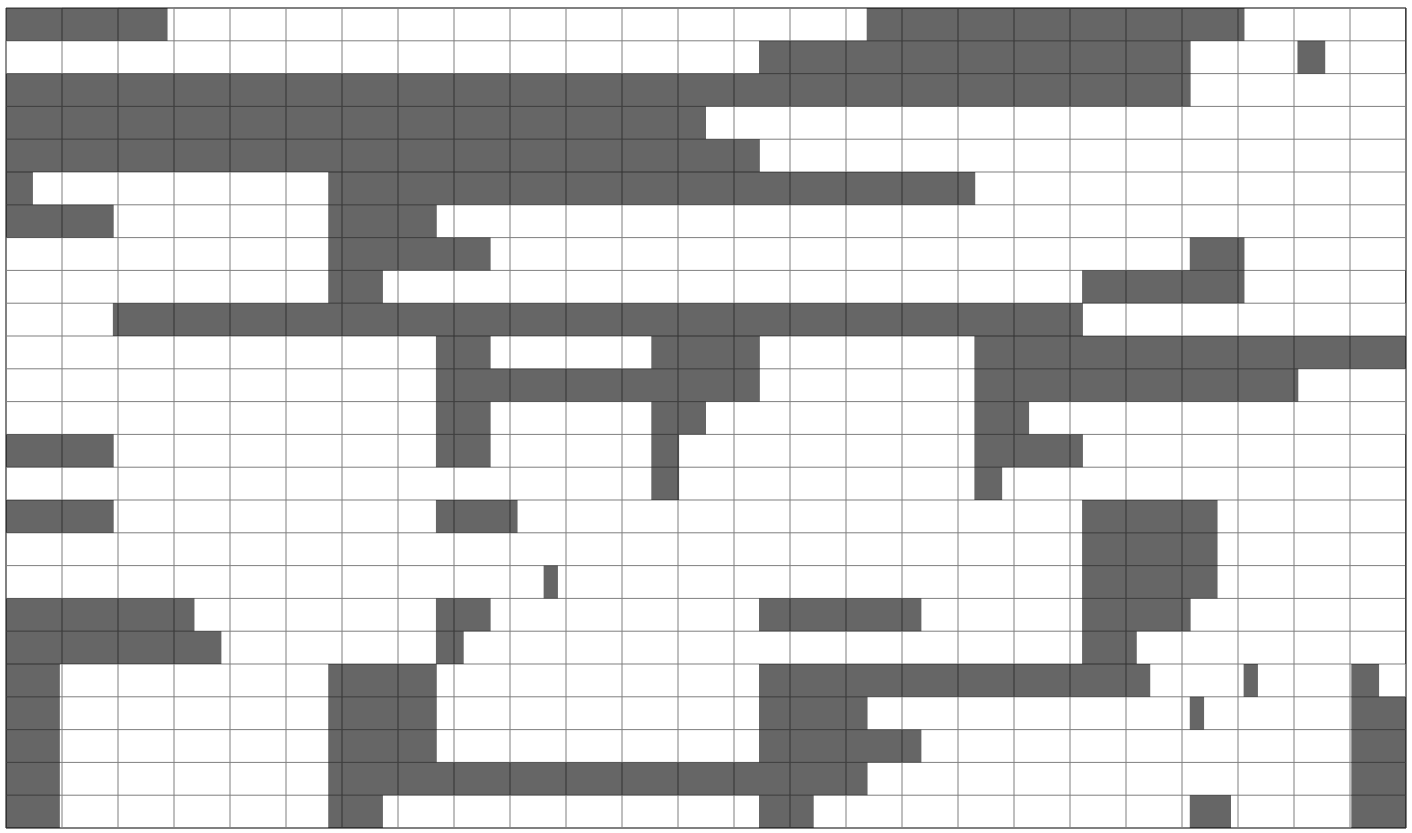
\includegraphics[width=16cm]{chapter5/midi_gesualdo.tif} %change centimeters for resizeing
   \caption{Visualization of Gesualdo's \emph{Se la mia morte brami}.}
   \label{fig:example}
\end{figure}\
This Midi file has five tracks which represent the different voices of the madrigal. The representation of the Midi file displays the silences in dark grey and the phrases in white. This is with the purpose of being able to consider the phrases as `empty containers' and write annotations in the printed result on what kind of `material' these containers may be filled with. That is to say, the result can be used as a sort of pre-compositional design for the new composition and the printed version allows the composer to make notes on different levels of decision making through time.\footnote{See \emph{Structure Maps} in DVDs I--III (they can be found in Documentation \tiny \textgreater \footnotesize \hspace{0pt} Performance Materials), for examples of compositions which used this application of \emph{macro} plundering the phrase structure from other compositions to create not only pre-compositional blue-prints for new compositions but also to be used as performance material (they were used as study material for performers or as `scores' to guide the musicians during the performance).}

\subsection{Midi Triggering}

Following the idea of using existing compositions as a blueprint for the design of a new work, I have continued to write applications that trigger events and processes through Midi messages. For example, these events or processes might be used to trigger and control synthesis definitions, Midi events and even real-time scoring. I have written various extensions of SimpleMIDIFile to use the messages from a Midi file for this objective. Therefore, these extensions employ a Midi file as a control structure for triggering functions of different types.
The extension \emph{playTrackType} plays different types of Midi events in a Routine. One can specify a track number, type of Midi event, function to be evaluated when the event is triggered, starting time for the Midi file and  value to change the tempo by multiplying it to the original tempo of the Midi file. The function that is evaluated contains as arguments the specifications of the Midi events---for example, Midi channel, note and velocity, which can be accessed by the user. Therefore, it is possible to use this values to control the events or processes of the new composition. Additionally, the \emph{sectionPlay} message uses the information obtained by \emph{trackSilence} to evaluate a function each time that a phrase or silence starts. Furthermore, the \emph{phrasePlay} message evaluates two different functions: the first is evaluated at the beginning of a phrase and the second at the beginning of a silence. This two extensions respond to the same arguments as \emph{playTrackType} and can be useful for controlling meta-structures. They can also be used by the AlgorithicScore class to give cues to performers or trigger score animations. 

Given that Midi files which are created with the information from a score are quantized and therefore can be lacking in expression for a given purpose, I have also designed similar applications that work with incoming Midi data from a human performer. Therefore, the computer can analyze the information in real-time and trigger events and processes that the composer programs before the performance. This type of application can be used in \emph{real-time plunderphonics} and \emph{live musica derivata}\footnote{See \hyperlink{realtimeplunderfuck}{pp. 93--94}.} as a strategy to control structures in a live performance.

%\section{Live-electronics}

%\subsection{Spectrum Driven Sampler}

%\subsection{Improvisation Environment}

In this chapter, I have briefly described the computer applications developed as part of the creative process during the period of research. Conclusion . . .

\label{ch:compapp}
%\hypertarget{chapter6}{}
\chapter{Compositions}

This chapter briefly describes the portfolio of submitted work. It focuses exclusively on technical and musical descriptions of the musical output and is not intended to serve as a wider commentary on the submitted work---the previous chapters already serve as a meta-commentary on the wider concerns underlying the creative process and musical output. This portfolio I believe reflects the various musical practices that I have been involved in during the research period, which include composing, improvising and performing as well as writing computer programmes. Furthermore, within my creative practice these different activities are often interconnected, resulting in work that is sometimes difficult to categorize using only these traditional definitions. Therefore, the submitted work also includes a wide variety of outcomes which may be identified as different types of work. I tried not to exclude any of the various types of musical outcome that make up my creative practice, although by doing so I am aware that my work might appear to lack focus. Nevertheless, I consider the diversity of outcomes from my practice to be a feature of my creative process and, instead of repressing this characteristic of my work, I attempt to embrace it. For that reason the type of work presented as part of this portfolio includes simple as well as more ambitious projects, some of which are ongoing and could be perceived as unfinished. As my work seeks to rework musical strategies that might be regarded as fundamental to the way in which we traditionally create, perform and experience music, my practice is necessarily experimental in nature and I consider it is important to present not only work which presents successful outcomes, but also failed and incomplete experiments. I have divided the portfolio of work in five main projects. The first project is \emph{E-tudes}, a set of four pieces for live electronics and six pianists playing keyboards, a work which can be presented as a concert performance or as an installation with performative elements. I will describe the basic set-up and computer programmes that are fundamental to the way in which all of the four pieces are performed and presented, later examining each individual `e-tude' in more detail. The second project I will examine is a piece called \emph{On Violence} for piano, live electronics, sensors and computer display. I will describe how this work is performed and how it was composed, including the way in which the multimedia score combines conventional with real-time notation and how the pianist interacts with the score, sensors and live electronics. The third project is \emph{\v{Z}i\v{z}ek!?}, a \mbox{computer-mediated-performance} for three improvisers that serves as an alternative soundtrack to a documentary about Slovenian philosopher Slavoj \v{Z}i\v{z}ek. I will explain how the improvisatory elements are incorporated within a pre-composed structure in this performance through real-time scoring strategies and how the final musical outcome is related to the audio of the documentary itself. The fourth project is a collection of short pieces called \emph{FreuPinta}. I will explain the nature of these small experiments, including the reason why I think they have aesthetic value on their own and belong with the rest of the submitted work. The experimental pieces fall into different groups based on their characteristics and I will briefly examine the reasoning behind their creation. Finally, I will briefly describe the fifth project which consists of a selection of different improvisations that I devised or participated in using the computer environment I developed for live improvisation.

\section{E-tudes}

\emph{E-tudes}\footnote{See \hyperlink{portfolio}{Contents of Portfolio}: CD I (\emph{Compositions}), Tracks 1--4 and DVD I (\emph{E-tudes}).} is a set of electronic \emph{\'{e}tudes} for six keyboards, live electronics and mechanical piano.\footnote{In case a mechanical piano is not available, it is possible to use a sampler with piano sounds.} These compositions were written for the ensemble \textbf{piano}\emph{circus}\footnote{See \href{http://www.pianocircus.com/}{\texttt{http://www.pianocircus.com/}}} for a project that became a \mbox{two-year} collaboration and led to two performances.\footnote{Enterprise 08 Festival, The Space, London, May, 2008, and The Sound Source, Kings Place, London, July, 2009.} What initially attracted me to this ensemble was its very particular instrumentation consisting of six electronic keyboards. I thought this would be a suitable platform to experiment with the notions of \emph{real-time plunderphonics} and \emph{live musica derivata},\footnote{See \hyperlink{realtimeplunderfuck}{pp. 91--92}.} considering that these instruments are electronic and therefore produce almost no audible acoustic sound.\footnote{The only acoustic sounds that can be heard are the keyclicks produced by the physical contact with the keyboards while playing. This noise is slightly audible mostly when there are no sounds playing through the speakers (or they are very quiet).} Like a book of \emph{\'{e}tudes} from the repertoire, \emph{E-tudes} consists of a set of pieces that can be performed together at the same event or individually as separate short pieces. At present I have completed four `e-tudes'; as it is an ongoing project, I will continue adding new pieces to the collection. \emph{E-tudes} is modular in the way in which it can be presented: depending on the set of circumstances for a given event, they can be presented separately or as a whole, as a concert performance or as an installation with performative elements. In the installation version, the audience walks into, out of, and around the area surrounding the musicians and has creative control over how they want to experience the performance. By choosing between listening to the speakers in the room or to various headphones which are distributed through the performance space and which generate different outputs, each member of the audience fabricates their own version of the piece. In the installation version there are various possible outputs generated by the computer from the performance from which the audience can choose. It is also possible to have a performance where the members of the audience are wearing wireless headphones that can receive multiple channels that are transmitted in the performance space, allowing them to choose which channel and output from the performance they want to hear.\footnote{This was the case in the performance at Kings Place.}

I use the same configuration for all of the pieces that comprise \emph{E-tudes}: the ensemble of six keyboards is placed in hexagonal formation and divided into two subgroups. The first subgroup, consisting of three pianists, are asked to select \emph{\'{e}tudes} from the western piano repertoire at will---they can select the \emph{\'{e}tudes} they prefer to perform (for example, \emph{\'{e}tudes} by Chopin, Debussy or Ligeti, to mention just a few)---and are asked to play them in their chosen order during the duration of the performance. The second subgroup, consisting of the remaining three pianists, perform together from \emph{The Sixth Book of Madrigals} by Don Carlo Gesualdo da Venosa (1566-1613). The pianists playing the madrigals send Midi information to a computer that transforms the audio signal from the \emph{\'{e}tudes} and schedules the computer-processing events. The audience is not be able to hear in the room what the pianists are playing as the keyboards do not produce an acoustic sound. The seventh performer (performing the live electronics part)\footnote{In the previous performances of \emph{E-tudes}, I have performed the live electronics part myself.} performs different tasks: at some points s/he speaks the Madrigals' text into a microphone and the spectral information from this signal is used to process the final audio output and to trigger other sound events; at other times s/he mixes the resulting sounds, controls different parameters in the computer processing and triggers sounds with a Midi controller. The live electronics part is not fixed, leaving space for improvisational elements within the human/computer interaction. Finally, through the analysis of all the inputs the computer sends Midi messages to the mechanical piano, adding yet another element to the performance. In the room the final result of the creative process of combining the simultaneous performances in diverse arrangements is diffused through the speakers. In the installation version, the headphones that are spread through the performance space portray the inner life of the performance sounding in the room and reveal the inner layers of computer processing as well as the appropriated compositions.

Computer programmes play a vital role in \emph{E-tudes} and were written in SuperCollider---some of these programmes are discussed in \hyperlink{chapter5}{Chapter 5} but some were exclusively written for \emph{E-tudes}.\footnote{The code for these computer programmes can be found at \href{http://github.com/freuben/Etudes}{\texttt {http://github.com/freuben/Etudes}}.} These programmes are used to analyze incoming Midi data to schedule events\footnote{See \hyperlink{miditrig}{p. 113}.} and for digital signal processing (DSP). The incoming Midi events from the pianists playing Gesualdo are analyzed and divided into each voice of the original madrigals. The computer uses score following techniques to track each voice and according to its position in the score, schedules specific DSP events. The Midi \emph{note} and \emph{velocity} information in some occasions is used to determine certain parameters in the DSP algorithms. The DSP algorithms of the live electronics use as input two major audio sources: the input of the combined live audio of the sound generated by the three pianists playing \emph{\'{e}tudes} and \emph{micro} elements\footnote{See \hyperlink{macroplunder}{pp. 89--91}.} derived from various recordings of existing music which I chose to appropriate. The individual live audio signals coming from each pianist playing \emph{\'{e}tudes} are interpolated\footnote{What I mean by interpolation is a transformation of one sound to another through a process that does not necessarily fit the description of `morphing'.} with one another (by altering the pitch and volume of the signals).\footnote{Each signal is interpolated with the other by gradually pitch-shifting one signal down four octaves and fading out its volume gradually, while at the same time introducing the next signal which would be pitch-shifted four octaves down and gradually transposing it up until its original pitch, and by gradually fading it in.} The live electronics performer can change the duration of the interpolation between \emph{\'{e}tudes} with the Midi controller. At the same time, the resulting signal is then pitch-shifted again through several pitch ratios (the original signal results in five different signals with varying pitch) generating multiple signals which are then mixed together. The sounding result is a very noisy signal which could be described as `piano noise' (it still retains a piano-like quality). I then utilize the `piano noise' as input in synthesis algorithms which filter it using several techniques. The `piano noise' is very different to \emph{white noise}, \emph{pink noise} or any other types of noise used in classic synthesis techniques in that its spectral flux is constantly changing and its rate and amount of change is fairly irregular. Additionally, the live electronics performer can change the sonic qualities of the `piano noise'---and therefore also change its spectral flux---by altering the interpolation time of the live audio signals coming from the pianists. Some of the `e-tudes' in their final result (the output diffused through the speakers) are composed exclusively using synthesis algorithms which use this `piano noise' as input. At the same time, in the installation version, the audience can listen through headphones to the different outputs at different degrees of processing---for instance, one of the headphone outputs consists entirely of material generated from the interpolation of \emph{\'{e}tudes}, while another one reveals the `piano noise'. In certain headphone outputs the original appropriated sources (the \emph{\'{e}tudes} and the madrigals by Gesualdo) also appear closer to their original form. The algorithms that control the overall process have generative elements---each time they are performed, they generate different results. The generative characteristics of the algorithms, the varying incoming data from the live performances (the \emph{\'{e}tudes} chosen by the pianists change for each performance of \emph{E-tudes}\footnote{Like Cage's \emph{Imaginary Landscape No.4}, this type of musical appropriation is current, generative and indeterminate. See \hyperlink{landscape4}{p. 81} for a further discussion of Cage's appropriation strategy.} and the incoming Midi data from the madrigals varies each time they are performed) as well as the improvisatory elements in the live electronics performer's part, makes \mbox{\emph{E-tudes}} an electronic composition that changes (both in content and performance) each time that it is presented, while also maintaining certain elements that identify it as the same composition.

\emph{E-tude I} is based on the first madrigal of Gesualdo's \emph{Sixth Book of Madrigals} called \emph{Se la mia morte brami}. In \emph{E-tude I}, `piano noise' is filtered in different ways using various subtractive synthesis algorithms. Several algorithms take the live electronics performer's voice reading the words of the madrigal as input to filter the `piano noise' using different filtering techniques. The most prominent filtering techniques using the voice as input are vocoding (using a variation of the `classic' vocoder algorithm) and the FFTFilter described in the previous chapter.\footnote{See \hyperlink{fftfilter}{pp. 98--99}.} The microphone signal is also used for onset detection, and the live electronics performer may trigger different percussive sounds (generated by filtering bursts of `piano noise' at different frequency ranges) with his/her voice. Spectral gating (an FFT technique which ignores the frequency bins which have magnitudes below a certain threshold) of a limited frequency range of the `piano noise' is another technique used to isolate the strongest frequencies in a specified range---the resulting frequencies are used as pitched material that is presented either in its natural sinusoidal quality (prominently in the high frequencies) or these frequencies are mapped into Midi notes which trigger the mechanical piano (mostly using its lower range). At the same time, all pitched material (including the center frequency of some filtered sounds) is altered or defined by the Midi note information received from the pianists performing the madrigal (tuned in \emph{just intonation}). The dynamics for these sounds are shaped by the Midi velocity from the performance of Gesualdo. At the same time, the different layers of sound are modified such that they have a similar phrase structure to the madrigal---the layers start and end at the same point in time as the madrigal.\footnote{I use this technique in many of my compositions: I plunder the phrase structure of an existing composition to generate a blueprint for a new composition. See \hyperlink{macroplunder}{pp. 89--90}. I also wrote a computer programme that automizes this process and generates a visual representation of phrase structure using a Midi File as input. See \hyperlink{scorevisual}{pp. 109--112}.} The Midi note information (mostly note-on messages, but not exclusively) at times also trigger different sounds generated through a combination of filtered `piano noise' and data derived from analysis of plundered recordings. A common technique used in \emph{E-tudes} to make synthetic sounds sound more imperfect or `natural' sounding is to modify the synthesized sound according to the extracted fundamental of a recorded instrumental or vocal sound---the synthetic sound becomes more irregular and therefore sounds more `natural' due to the imperfection it inherits from the instrumental or vocal sound. Another technique I use to make synthesis algorithms sound more `instrumental' is by deriving harmonic structures (the fundamental and partials of a sound) from FFT analysis of recordings of the instruments I want to approximate. In \emph{E-tude I}, I generate sounds using these techniques to approximate sounds with similar characteristics to a celesta, several percussion instruments, to a vocal melody, high bowed string harmonics, etc. I also use FFT to combine spectra between the instrumental recordings and the `piano noise'. \emph{E-tude I} starts with a fairly `abstract' sound world---further removed from recognizable `traditional' instruments or music genres and including sounds that are more noise than pitch based---gradually transforming into a more `referential' sound world, made up of pitched sounds, periodic rhythms, more identifiable sounds modeled on existing instruments and pitch material that is more referential to other more recognizable musical genres. The process of transformation culminates with the emergence of a prominent melody (driven by the FFTFilter, filtering `piano noise' and following the melodic contour of a plundered recording of a vocal sound) resulting in music that is reminiscent of a song (or aria) with an \emph{ostinato} of simple and `primitive' rhythms.

\emph{E-tude II} uses \emph{Belt\`{a} poi che t'assenti} (the second madrigal in the book) as the control structure of the computer processing. In this `e-tude', the role of the `piano noise' is reduced only to a source of noise within physical modeling synthesis algorithms, which create sounds reminiscent of instrumental sounds. These sounds include the high frequency sound based on a physical model of a bowed string which ended \emph{E-tude I}, this time changing in pitch more gradually and gliding through what sounds like a variation of the main melody of the `song' with which \emph{E-tude I} culminates. The algorithms generate sounds reminiscent of plucked strings, percussion and wind instruments based on physical models of Korean instruments. The `plucked string' sounds, for instance, are generated using a variation of the Karplus-Strong plucked-string algorithm using a burst of `piano noise' as its excitation and altering it in frequency and amplitude through the extracted fundamental of a recording of a plucked \emph{Geomungo} (Korean instrument) string. In addition to the sounds generated by the synthesis algorithms, the mechanical piano produces pitched material consisting of ascending \emph{arpeggios} generated through vowel sounds that are \emph{synthrumentized}, which the live electronics performer vocalizes into the microphone.\footnote{The PartialTracker class is used to detect the strongest frequencies of these vowel sounds to generate notes for the \emph{arpeggios}, see \hyperlink{partrack}{p. 97}.} The prominent melodic sound that emerges on its own at approximately the middle of \emph{E-tude II}, is generated through a combination of `classic' filtering techniques (band pass, high pass, dynamic bank of resonators, etc.) which filter the `piano noise' to try to emulate a `wind instrument' with vocal characteristics. The attack and release envelopes of this sound are derived from a recording of a recorder and after the sound is released, a high-frequency noise reminiscent of human breathing follows (the frequency range of the noise was mapped approximately to the frequency range of a person's breathing-in sound). This `virtual instrument' plays a melody that is plundered from a recording of \emph{Gagok}---a traditional form of Korean vocal music.\footnote{See \hyperlink{rockwell}{Rockwell (1972)} for an introduction to \emph{Gagok}.} After a brief solo section, an ensemble of `virtual instruments' joins the melodic sound and emulates music reminiscent of \emph{Gagok}---including two `virtual instruments' (one of them sounds more `sinusoidal' and the other sounds closer to a reed instrument) that play the melody with slight deviations in timing and tuning. These deviations are driven by a generative algorithm (meaning that each time that \emph{E-tude II} is performed, the melodic deviations vary) that is designed to emulate the types of improvised melodic elaborations found in original \emph{Gagok}. During the duration of \emph{E-tudes II}, the rate at which sporadic events (plucked strings, percussion instruments and mechanical piano \emph{arpeggios}) take place gradually becomes faster and the events themselves become more active and unpredictable (for instance the mechanical piano \emph{arpeggios} become faster and with more notes and their direction starts changing randomly as they become more active), until they are squashed against each other and become cluttered at the end of the composition.

\emph{E-tude III} is based on the third madrigal by Gesualdo called \emph{Tu piangi, o filli mia}. This `e-tude' opposes synthesized pitched sounds with a strong fundamental frequency (some of them sound almost like sine waves) at the beginning with the `piano noise' that is revealed for the fist time in its unfiltered and unprocessed form later in the composition. The pitched sounds consist mainly of three different types of sounds: two sustained sinusoidal pitches, `celesta' sounds and a single descending \emph{arpeggio} of `plucked string' sounds. The two sinusoidal pitches slowly change in frequency, first gradually detuning away from each other and later changing direction until they slowly approach each other, producing \emph{beating} before merging into the same tone. The `celesta' sounds are generated in the same way as the ones that were used in \emph{E-tude I} (generated from filtered `piano noise') and derive their pitch material from spectral data (\emph{Synthrumentation}) of the audio signal of just one of the pianists playing \emph{\'{e}tudes}. Their rhythm is triggered through onset detection of the live microphone signal (the voice of the live electronics performer reading the text of the madrigal). The descending \emph{arpeggio} of `plucked string' sounds---which happens only once and is reminiscent of the mechanical piano \emph{arpeggios} in \emph{E-tude II}---is generated through the same Karplus-Strong algorithm used in \emph{E-tude II}, but instead of using a plundered recording of a \emph{Geomungo}, it uses a recording of a harp. The `piano noise' is first revealed as short percussive sounds (the `piano noise' is filtered so that it sounds like footsteps) triggered by the live electronics performer with the Midi controller at periodic intervals. Then it is revealed as filtered noise in the high frequencies and later in the low frequencies---the filtered noise originates from a selection of FFT bins of `piano noise'. In \emph{E-tude III}, there is a slow transition between pitched sounds and `piano noise', which gradually becomes dominant as the spectrum is gradually filled with FFT bins---culminating in the complete frequency spectrum of `piano noise' being diffused equally over the speakers. At the end, the `piano noise' vanishes completely in a matter of seconds (through the reverse FFT process) followed by silence, and a series of sporadic and aggressive bursts of clusters played by the mechanical piano and by short phrases of sinusoidal sounds and \emph{synthurmentized} piano chords revealing harmonies from the \emph{\'{e}tudes}. 

\emph{E-tude IV} derives information from three main sources: Gesualdo's forth madrigal called \emph{Resta di Darmi Noia}, the \emph{\'{e}tudes} chosen by the pianists and several appropriated recordings of Pygmy music.\footnote{\hyperlink{pygmy}{Mbuti Pygmies of Ituri Rainforest (1992)}.} Pitched material is derived from recordings of Pygmy music using the SpearToMIDI and PartialTracker programmes described in the previous chapter.\footnote{See \hyperlink{spectrack}{pp. 95--103}.} The results from the different types of analysis are then selected and combined according to the desired musical outcome and stored as Midi note data. The spectral data of the \emph{\'{e}tudes} is combined with the collected data from the Pygmy music recordings and the result is modified by the melodic and harmonic material from the madrigal. The Midi information resulting from this process is realized by the mechanical piano, which is the only source producing sound, becoming the `virtual' soloist of \emph{E-tude IV}. At some points, the melodic contour from the different voices from the Gesualdo is used to modify the tempo of the different layers of the Midi note data derived from the Pygmy music---if the shape of melody goes up, the tempo progressively becomes faster and if the melody goes down, the tempo becomes slower. In addition, certain algorithmic composition strategies are used to process the final result---for example, stochastic methods are used to control note density by gradually filtering notes \emph{in} and \emph{out}. \emph{E-tude IV} uses data of three recordings of Pygmy music, which at the same time represent three sections of the composition. The first section is based on a song for the \emph{molimo} ritual,\footnote{Ibid., Track 24.} which is celebrated on special occasions such as the death of an important member of the tribe and is meant to wake up the forest from the sleep which is allowing bad things to happen to its children.\footnote{See \hyperlink{mukenge}{Mukenge (2002)}.} The middle section is based on a recording of a musical bow played by a \emph{Mbuti} pygmy,\footnote{\hyperlink{pygmy}{Mbuti Pygmies of Ituri Rainforest (1992)}, Track 15.} which morphs into the last section, derived from a recording of hunters signaling, shouting and beating.\footnote{Ibid., Track 5.}

\emph{E-tudes} is a set of compositions that explores a type of live electronics performance which attempts to establish new relationships between performer, composer and audience. It establishes at different times both \emph{interactive} and \emph{interpassive} relationships between the performer and the technological objects as well as between the musicians and the audience.\footnote{See \hyperlink{newrelationships}{pp. 46--52}.} It also seeks to establish new forms of exchange between composer and performers as well as between the performers within an ensemble.\footnote{See \hyperlink{ensembledy}{p. 53}.} \emph{E-tudes} combines the use of live electronics, improvisation, real-time computation and generative music to create a result which is unfixed, responsive and which changes for each performance of the work.\footnote{See \hyperlink{techcomp}{pp. 53--56}.} Additionally, \emph{E-tudes} attempts to find new and innovative ways to approach the process of appropriation using idiosyncratic musical strategies. First, it plunders live performances of existing music, using their audio and Midi signals as building blocks for multiple musical results, exploring the notions of \emph{real-time plunderphonics} and \emph{live musica derivata}.\footnote{See \hyperlink{realtimeplunderfuck}{pp. 91--92}.} It also appropriates \emph{micro} and \emph{macro} elements of notated material, recordings and live signals as well as treating the musical sources at varying degrees of processing, affecting our ability to recognize the original source. Finally, the sources from which \emph{E-tudes} appropriates are, unlike classic \emph{plunderphonics}, indeterminate, less familiar, obscure or exotic: music from places far removed from western culture (Korean traditional vocal music, Pygmy Music), early music (Gesualdo madrigals), pop music far from the mainstream of consumer culture and unspecified \emph{\'{e}tudes} from the repertoire.\footnote{See \hyperlink{appropstrat}{pp. 88--91}.}

\section{On Violence}
 
 \emph{On Violence}\footnote{See \hyperlink{portfolio}{Contents of Portfolio}: CD I (\emph{Compositions}), Track 5 and DVD II (\emph{On Violence}).} is a composition for piano, live electronics, sensors and computer display.\footnote{The code of the programmes that run \emph{On Violence} can be found at \href{http://github.com/freuben/OnViolence}{\texttt {http://github.com/freuben/OnViolence}}.} The pianist reads from a score displayed on the laptop screen, which combines conventional notation with real-time scoring.\footnote{See \hyperlink{realtimescore}{pp. 103--104} for a discussion on real-time scoring strategies.} The performer also wears headphones to receive audio triggers and cues that constitute the aural element of the score. I implemented this score using SuperCollider and the AlgorithmicScore class.\footnote{See \hyperlink{algoscore}{pp. 104--109}.} The pianist interacts with the score through two midi pedals that are used to `turn pages', display graphic notation, give written directions to the performer and activate score animations. During the duration of the performance, the score gradually alters from conventional notation to more experimental notations.\footnote{See DVD II (\emph{On Violence}) \tiny \textgreater \footnotesize \hspace{0pt} Documentation \tiny \textgreater \footnotesize \hspace{0pt} Score Demo for a demo of how the score might look/sound during performance.} The real-time scoring elements of \emph{On Violence} use a combination of chance, generative and spectral methods to generate visual and aural material that changes and adapts for each performance. The pianist therefore is asked to follow a score that has both fixed and unfixed indications, some of them involving spontaneous reaction and improvisation. The score information is generated in real-time by the computer and is very difficult, if not impossible, to perform accurately since the pianist does not know the exact content of the music s/he will be performing. However, the pianist is still asked to perform the score to the best of his/her ability. This type of performance strategy is deliberate and attempts to establish an \emph{interpassive} relationship between the performer and the laptop displaying the score---the pianist becomes frantically active by the `impossible' demands from the technological object which remains passive.\footnote{See \hyperlink{zizekinterpassiv}{pp. 48--49}.}

\emph{On Violence} appropriates existing music form various sources: Dieterich Buxtehude's \emph{Praeludium in G Minor, BuxWV 132}, Einst\"{u}rzende Neubauten's \emph{Autobahn} and Richard Wagner's \emph{Parsifal} and \emph{Tristan und Isolde}. It also plunders sounds including political speeches, screams, guitar feedback and metal banging. Buxtehude's \emph{Praeludium} serves as a blueprint for the composition---the other derived material is placed within its form, and is treated and processed through its shapes and contours as well as its melodic, harmonic and contrapuntal content. The live electronics part is triggered by the audio analysis of the music performed by the pianist (a microphone is placed close to the piano for real-time analysis) and by the Midi pedals. Through a combination of \mbox{machine-listening} technology and by tracking the incoming data from the Midi pedals the computer is able to follow the score, triggering different sounds and types of processing according to the structure of the composition. There are various predominant sounds in the live electronics part at the beginning of the composition: metaling bangs, vocal sounds (screams and fragments of political speeches, some of which are heavily processed), high frequency distorted sounds and a sound reminiscent to the noise produced by a motor. The metal bangs are triggered through the onset detection of the piano signal and are stretched or shortened in real-time depending on the speed at which the pianist plays. The samples of vocal sounds and the high frequency distorted sounds are selected randomly and triggered at specific moments following the pianist's playing and are also stretched or shortened in real-time depending on the tracked tempo. Some of the vocal sounds are processed by two different types of synthesis algorithms: one of them convolves two different types of weakly nonlinear oscillators which use the sample as its external force and the other convolves one weakly nonlinear oscillator with the result of a linear predictive coding (LPC) error.\footnote{The UGens used in these synthesis definitions are part of the SuperCollider SLUGens library by Nick Collins.} The high frequency sounds are spectrally gated samples of guitar feedback that are passed through a distortion guitar pedal. The sound reminiscent of a motor is turned on and off through the Midi pedals and consists of a low frequency pulse wave that is distorted through an overdrive guitar pedal. The pianist controls the frequency of the pulse wave with two 3G Force sensors (accelerometers) attached to his/her hands, which track arm movement (as the pianist lifts his/her arms, the frequency increases and as s/he lowers them, the frequency decreases). During the first section of the composition, the pianist alternates between incessantly banging chords at a periodic rhythm and controlling the `motor' sound by lifting and lowering his/her arms. The chords that s/he plays are derived from the spectral analysis (using the PartialTracker class) of Neubauten's song \emph{Autobahn} and modified both in harmonic material and register by the Buxtehude. The pitched material of the vocal and distorted high frequency sounds as well as the `motor' sound are also modified in pitch through the Buxtehude score. As the pianist's score starts to incorporate more real-time scoring elements the content of the live electronics part also gradually starts to transform. Samples of plundered recordings of Wagner's \emph{Parsifal} and \emph{Tristan und Isolde} start to emerge, however modified in their playing rate by the mapped shapes of Buxtehude's counterpoint. The Wagner samples become more prominent as the pianist is asked to improvise and react immediately to the algorithmic score, culminating in an electronics solo that is produced by a synthesis algorithm emulating an organ sound and playing notes derived from a fragment of a recording of Buxtahude that corresponds to that precise section in the blueprint. After the electronics solo the performer responds by playing the next phrase of the original Buxtehude on the piano. The composition ends with the following section, where the pianist is asked to improvise freely together with an electronic part that consists of a re-synthesized version of the prelude to the third act of \emph{Parsifal}. The synthesis algorithm used in the electronics in this section uses a dynamic bank of resonators filtering noise\footnote{I created this noise using the same algorithm I used to generate `piano noise' in \emph{E-tudes}, however controlling its amplitude with low frequency noise, to emulate bowing.} and modified in frequency and amplitude by the extracted fundamental of the instruments in a plundered recording of the Wagner, resulting in a sound that approximates a bowed string instrument. This synthesis algorithm is then used to emulate a string orchestra by programming it to perform the parts of the different instruments of the string orchestra (violins, violas, cellos, double basses) and by multiplying its results by the amount of instruments per section and adding a slight random deviation in pitch and timing for each result to imitate the sound of various instruments playing in unison. The resulting version of the Wagner prelude however is altered in pitch content to match the previous section and for that reason the notes of the original are modified through the Buxtehude harmonic material.
 
This composition is inspired by Slavoj \v{Z}i\v{z}ek's book \emph{Violence},\footnote{See \hyperlink{zizekviolence}{\v{Z}i\v{z}ek (2008)}.} in which he categorizes violence into two main types: subjective and objective violence. Subjective violence is clearly identifiable by an agent, for example acts of terror or crime, and it is perceived as a clear interruption of the normal state of things. On the other hand, objective violence is violence that is inherent in the social fabric and is hard to see and experience for the advantaged classes or countries. What \v{Z}i\v{z}ek argues is that objective violence is inherent within social ``balance'' and it is objective violence which triggers acts of subjective violence. Furthermore, \v{Z}i\v{z}ek identifies two types of objective violence: symbolic and systematic violence. Systematic violence is manifested through our economic and political systems which, in order to give the idea of a normal smooth running of things, exert systematic violence on large groups of people. Symbolic violence is related to and included within systematic violence but is specifically expressed through language (and other symbolic systems like music). \v{Z}i\v{z}ek goes further to argue that the forms of symbolic violence are actually based on and manifested by the symbolic systems themselves.\footnote{Ibid. pp. 8--63.} \emph{On Violence} attempts to explore the aesthetics of violence and reflect on the different manifestations of violence categorized by \v{Z}i\v{z}ek. It does so, not only through the type of sounds and plundered music it uses (which are suggestive of different types of violence) and the way they are processed, but also through the way in which the performance itself is set up. The pianist is asked to be violent by the sheer force and agressiveness s/he has to exert over the instrument and further violence is exerted upon him/her by the amount of information that is thrown at him/her by technology and by the pressure of having to perform difficult (if not impossible) tasks. Even though at the beginning of the composition, it seems that the pianist is the one exerting subjective violence onto the piano and controlling technology---by triggering sounds through pedals and controlling the `motor' sound through the sensors---we later realize that technology is controlling the pianist by flooding him/her with impossible demands. At the end of the composition, while the pianist is apparently free (s/he is asked to improvise freely and play what ever s/he wants) we get the impression that s/he is not the one in control and actually is the victim of objective violence imposed systematically upon him/her, not only by the system of performance and technology but also by the symbolic violence implicit in the music itself.

\section{\v{Z}i\v{z}ek!?}

\emph{\v{Z}i\v{z}ek!?}\footnote{See \hyperlink{portfolio}{Contents of Portfolio}: CD I (\emph{Compositions}), Track 6 and DVD III (\emph{\v{Z}i\v{z}ek!?}).} was commissioned for an event about the Slovenian philosopher Slavoj \v{Z}i\v{z}ek, which took place at The Sound Source, Kings Place, London, July, 2009. I was commissioned to write a live alternative soundtrack to Astra Taylor's \emph{\v{Z}i\v{z}ek!} (2005) documentary, which resulted in a \mbox{computer-mediated-performance} for three improvisers performing on piano, double bass and drums.\footnote{It was premiered by Alexander Hawkins (piano), Dominic Lash (double bass) and Javier Carmona (drums).} In \emph{\v{Z}i\v{z}ek!?}, each improviser has a laptop in front of them, connected through a computer network, by which the improvisers receive individual written directions, timing instructions, score animations (moving graphical notation) and through headphones an aural score that consists of music they have to interact with.\footnote{See DVD III (\emph{\v{Z}i\v{z}ek!?}) \tiny \textgreater \footnotesize \hspace{0pt} Documentation \tiny \textgreater \footnotesize \hspace{0pt} Performance Materials \tiny \textgreater \footnotesize \hspace{0pt} Score Parts.} The result is a real-time multimedia score that is synchronized with the film and is driven by computer programmes written in SuperCollider,\footnote{The code of the programmes that run \emph{\v{Z}i\v{z}ek!?} can be found at \href{http://github.com/freuben/Zizek}{\texttt {http://github.com/freuben/Zizek}}.} including the AlgorithmicScore class discussed previously.\footnote{See \hyperlink{algoscore}{pp. 104--109}.} The improvisers receive seven different written directions through the laptop displays, telling them how they should react during the performance:
\begin{enumerate}
\item \emph{Silence}: Don't play (or stop playing).
\item \emph{Like}: Imitate the music coming from the headphones.
\item \emph{With}: Play together with the music coming from the headphones.
\item \emph{Free}: Free to improvise at will.
\item \emph{Solo}: Improvise a solo.
\item \emph{Unlike}: Play in opposition to the music coming from the headphones. 
\item \emph{Without}: Improvise ignoring the sound from the headphones.
\end{enumerate}
The letters of the written directions are also color coded using the three colors of a traffic light: the \emph{Silence} direction is always in \emph{red} meaning the improvisers should stop playing at that point and the other directions are displayed in \emph{green} when they should play and \emph{yellow} when the \emph{Silence} direction is about to come. The performers also receive a written indication of which scene of the film is playing at a specific moment in time. The letters of these indications are in \emph{blue} while a specific scene is playing but turn \emph{pink} just before the next scene is about to start. In addition to written directions and indications, the multimedia score also includes score animations, which consist of moving graphical scores that convey some type of activity or gesture.\footnote{See \hyperlink{algoanimation}{pp. 107--108}.} Each score animation is deliberately devised for a specific instrument and is open to interpretation by the performer.\footnote{See DVD III (\emph{\v{Z}i\v{z}ek!?}) \tiny \textgreater \footnotesize \hspace{0pt} Documentation \tiny \textgreater \footnotesize \hspace{0pt} Score Animations for the interpretation of the animations by the improvisers during the performance.} The written directions, audio score and score animations are triggered through a control structure derived from a Midi file of Johannes Ockeghem's \emph{Missa Mi-mi} (using computer-aided-composition tools described in the previous chapter).\footnote{See \hyperlink{compueraided}{pp. 109--113}.} The music of the aural score, to which the improvisers have to react, is based on different types of analysis and processing of the audio of the film; it is not only synchronized to the film's audio, but it is derived from it. The music within the aural score is the result of different types of analysis from the speech, music and other sounds that comprise the film's soundtrack. Pitch and rhythmic material as well as frequency content and dynamics are derived from the analysis of the audio signal of the soundtrack using different techniques, including tempo tracking, onset detection and spectral analysis (PartialTracker and SpearToMidi classes)\footnote{See \hyperlink{spectrack}{pp. 95--103}.} and are combined/modified through the information obtained from the Ockeghem Midi file. This process generates data structures that control synthesis algorithms or triggers sampled sounds to create the final aural score. The result is an audio score that, while retaining some characteristics of the speech and other sounds from the film, is also allusive to other styles of music as a consequence of the chosen sounds and analysis parameters.\footnote{See DVD III (\emph{\v{Z}i\v{z}ek!?}) \tiny \textgreater \footnotesize \hspace{0pt} Documentation \tiny \textgreater \footnotesize \hspace{0pt} Score Demo.} The way in which the improvisers react to the audio score also produces an audible musical result that is related to the characteristics of speech and other sounds in the soundtrack and creates an interaction between the musicians and the sound of the film, which they might carry into the free improvisations.

\emph{\v{Z}i\v{z}ek!?} attempts to find new ways of collaborating with musicians with a background in improvisation by using computer-mediated-performance strategies that take advantage of their strengths as musicians but at the same time working within a pre-composed structure. It does so by reshaping the traditional relationships established between composer and performer through technology by using a multimedia score to transfer musical ideas and intention as well as facilitating certain types of group playing and synchronicity that otherwise would be difficult to achieve.\footnote{See \hyperlink{superscore}{pp. 39--42} for a discussion about the possibilities of using technology to produce a multimedia score which facilitates communication with and between musicians from different backgrounds.} In addition, by giving the improvisers visual directions and aural stimulus, it is possible to direct them towards a certain type of musical behavior and sound world without limiting their creative input into the performance. Furthermore, \emph{\v{Z}i\v{z}ek!?} is devised in such a way that, within a fixed structure, certain details may vary through improvisation, but within the constraints given by the visual and aural score. This computer-mediated-performance shares certain characteristics with generative music: the composer does not specify every detail of the result of the performance but creates the possibility for an infinite number of outcomes which share similar characteristics.\footnote{See \hyperlink{realtimepos}{pp. 54--56} for a further discussion about the relationship between improvisation and real-time computation, generative music and interactive systems.} \emph{\v{Z}i\v{z}ek!?} also explores the idea of establishing \emph{interpassive} relationships between the performers on stage and the technological objects (the laptops in front of them).\footnote{See \hyperlink{interpassiv}{pp. 46--50}.} Like \emph{On Violence}, this performance is devised in such a way that the technological object remains passive (the laptops do not produce sound or activity that is apparent to the audience) while requiring the performers to remain (hyper)active. The improvisers delegate their passivity to the technological object, giving the semblance of reality to the illusion that they are in control, when they are actually following the demands from the laptops. Finally, \emph{\v{Z}i\v{z}ek!?} deals with the process of appropriation slightly differently from \emph{plunderphonics} or \emph{musica derivata}. The composer creates a new musical result by appropriating live performances as opposed to creating music through plundered recordings or by writing a score based on derived material from existing music to be realized by either classically trained musicians or mechanical instruments. This is achieved by appropriating the performance of musicians with a background in improvisation and by manipulating the output of their improvisation through the multimedia score. \emph{\v{Z}i\v{z}ek!?} appropriates live performances differently from \emph{E-tudes}; instead of plundering different types of signals from live performances to create a new composition the process of appropriation starts by choosing living improvisers (rather than recordings, audio and Midi signals of existing music), manipulating/directing their creative output towards a desired musical result. Furthermore, \emph{\v{Z}i\v{z}ek!?} appropriates a film into the performance and superimposes live music on top of its original soundtrack so that the live music performance interferes with the appreciation of film by trying to steal the audience's attention from it. The activity and volume of the improvisation (the music is meant to be louder than conventional film music, sometimes masking the audio of the film) at some points competes with \v{Z}i\v{z}ek's own relentlessness as a speaker. At the same time, however, as a consequence of the relationship between the live music and the audio of the soundtrack, the performance amplifies \v{Z}i\v{z}ek's own hyperactivity, suggesting that he is not the analyst but the analysand. The result of the performance as a whole is an overload of information for the audience who, not being able to grasp the whole content of the performance (the meaning of the concepts being discussed, the images of the documentary and performance, as well as the detail in the music) has to give something up---the audience might (consciously or unconsciously) decide to ignore the music in order to try to concentrate on understanding what is being said or might choose to perceive the performance as sound, rendering \v{Z}i\v{z}ek's speech as music and detracting from its meaning as language. The audience may also have to come to terms with the impossibility of fully grasping what is presented at them, stop trying to understand all of the different elements of the performance and perhaps give up on it entirely, becoming passive spectators of an `empty ritual'.

\section{FreuPinta}

\emph{FreuPinta}\footnote{See \hyperlink{portfolio}{Contents of Portfolio}: CD II (\emph{FreuPinta}).} is a collection of small experimental pieces that were realized in parallel to the more ambitious musical projects. They are often small experiments, studies, fragments and residues of the bigger pieces. By themselves they might not be considered as significant achievements but, nevertheless, I consider they still have some aesthetic value on their own. During the research period, I produced several of these short musical experiments in parallel to some the main computer programmes I developed, often as a testing bench of their functionality.\footnote{See \hyperlink{chapter5}{Chapter 5} for a short description of these computer programmes.} The aesthetic value of these pieces lies, I believe, in that they were developed as consequence of an experimental process that I think reflects my broader aesthetic concerns. Many of these short experiments are concerned with finding new interesting approaches to musical appropriation.\footnote{See \hyperlink{chapter4}{Chapter 4} for a discussion of musical strategies that deal with appropriation as a creative tool.} The way in which they deal with the process of appropriation is often more `straightforward' than the rest of the submitted work and reveals more directly and apparently the appropriation of only one piece of existing music. Many of these pieces are the result of documented experiments in the development of computer programmes that aimed at finding new types of relationships between performer, composer and audience through technology.\footnote{See \hyperlink{chapter3}{Chapter 3} for a further discussion on how technology might help reshape relationships between people involved in making and experiencing music.} A considerable number of pieces from this collection were also the result of experiments in generative, spectral and other algorithmic techniques that were implemented using real-time computation and interactive systems. \emph{FreuPinta} was also the platform where I first experimented with synthesis algorithms and physical models before implementing them in the bigger projects. My first experiments with \emph{real-time plunderphonics} and \emph{live musica derivata} are also documented as part of this collection of short pieces.

Some of the pieces that comprise the \emph{FreuPinta} collection are divided into different series of works. The \emph{simulation series} is comprised of four short pieces that deal with appropriation by attempting to simulate human performances of existing music through technology. `Artificial' performances are therefore created by appropriating recordings of human musicians playing different types of music and attempting to emulate these performances using tools provided by digital technology. The process of simulating human performance however is not with the purpose of reproducing the original music but of transcribing the music to be realized by `virtual' performers. The `artificial' performance is realized by analyzing the recording of the original performance using SpearToMidi\footnote{See \hyperlink{spearmidi}{pp. 101--103}.} (using different analysis parameters) to generate a `virtual' score that may be performed either by synthesis algorithms that emulate acoustic instruments or by mechanical instruments. For instance, \emph{Simulation No. 1} is a `virtual' performance of the overture to Handel's \emph{Solomon} oratorio realized by the computer using different `intrumental' sounds, therefore transcribing and `re-orchestrating' the original version. The process of transcription from the version performed by humans to the computer performance also introduces new sounds, pitches and rhythms that are idiosyncratic to the computer medium. \emph{Simulation No. 2} is a simulation of Radiohead's \emph{Pyramid Song} which derives data from the original recording that is performed by a mechanical piano. \emph{Simulation No. 3} and \emph{Simulation No. 4} present material that did not make it to the final version of the electronic part of \emph{On Violence}. They are simulations that use synthesis algorithms (which emulate an organ and a string orchestra respectively) that perform music derived from the computer's analysis of short fragments of recordings of Wagner (Prelude to third act of \emph{Parsifal}) and Buxtehude (\emph{Praeludium in G Minor}). The \emph{occupation series} comprises of three short pieces that deal with appropriation in a similar way: they appropriate a recording which is not processed or transformed at all and is left in its original form, however adding new sounds on top of the recording that are mixed with the original.\footnote{This series therefore uses a strategy similar to Duchamp's notion of \emph{assisted readymades}. See \hyperlink{lhooq}{pp. 65--66}.} The added sounds at the same time are also derived from the analysis of the recordings and are documented `performances' that use real-time computation---I used PartialTracker\footnote{See \hyperlink{partrack}{p. 97}.} and onset detection algorithms with different varying parameters that I had control over during the performance to trigger the new sounds. These sounds were recorded and mixed with the original, recontextualizing the meaning of the appropriated musical source. \emph{Occupation No.1} is a small personal homage to Stockhausen's \emph{Hymnen}---it appropriates the recording of the national anthem of Costa Rica (which is missing from Stockhausen's piece) and adds \emph{synthrumentized} piano chords on top of it. \emph{Occupation No.2} is a study for \emph{\v{Z}i\v{z}ek!?} which adds instrumental sounds (sampled guitar and percussion instruments) and sine waves to the recording of a lecture by \v{Z}i\v{z}ek---the instrumental sounds at the same time are derived from \v{Z}i\v{z}ek's speech. \emph{Occupation No.3} appropriates a fragment of Giovanni Palestrina's \emph{Missa Papae Marcelli} and adds a `virtual' jazz trio that `swings' along with the original. The \emph{transgression series} uses a different approach to the process of appropriation: it plunders data from the original source and then rearranges and reshuffles its components, re-imagining the original composition by transgressing its symbolic space. \emph{Transgression No. 1} re-imagines the first movement of Mozart's \emph{Sonata in C KV 545, I}, while \emph{Transgression No. 2} envisions an alternative version of the third movement of Bartok's \emph{Suite, Op.14, Sz62}. The remaining pieces in the \emph{FreuPinta} collection include more experiments controlling synthesis algorithms with data derived from spectral analysis of existing music (\emph{Chorus I}, \emph{Chorus II} and \emph{Artaud Dei}), my first experiments with the notions of \emph{real-time plunderphonics} and \emph{live plunderphonics} (\emph{Canzione Piramide}), experiments with interactive systems for live improvisation (\emph{Pianpeta}, \emph{Robojazz} and \emph{Sporcizia Vocale}) and mapping data from language and robotic movement to music (\emph{Danzonne} and \emph{Walking Head}).

\section{Improvisations}

The improvisations presented as part of the submitted work\footnote{See \hyperlink{portfolio}{Contents of Portfolio}: CD III (\emph{Improvisations}) and DVD IV (\emph{Improvisations}).} are the outcome of the work I have done in collaboration with other improvisers using the computer environment I developed in SuperCollider for live improvisation.\footnote{See \hyperlink{improvprog}{p. 113}.} The recordings of these improvisations are the result of several concerts and rehearsals that took place during the period of research. The submitted work includes recordings of several performances:
\begin{enumerate} 
\item \emph{Live@ICA}: concert of improvised music for a live performance art event called \emph{The Scuttler} presented by boyleANDshaw, which took place in June, 2010 at the Institute for Contemporary Art (ICA) in London. Free improvisation for live electronics, percussion, processed voice and guitar.\footnote{The performance featured Javier Carmona (percussion), Adam de la Cour (voice/guitar) and Federico Reuben (live electronics).}
\item \emph{Too Hot to Handel}: I was asked to present a work at the Handel House Museum. The museum is located on the upper floors of 25 and 23 Brook Street in London. 25 Brook Street was the residence of George Frideric Handel between 1723 and 1759 and 23 Brook Street was the home of Jimi Hendrix from 1968 to 1969. I decided to present a site-specific event that combined the music of both Handel and Hendrix simultaneously within a structured improvisation for live electronics, voice, guitar, harpsichord, drums, double bass and narrator/conductor.\footnote{The performance featured Adam de la Cour (voice/guitar), Alexander Hawkins (harpsichord), Javier Carmona (drums), Dominic Lash (double bass), Steve Potter (voice/conductor) and Federico Reuben (live electronics).}
\item \emph{Horatio Oratorio}: \emph{Horatio Oratorio} is a performance and sound installation that employs archival sound sources, including some of the first recorded utterances and music. The music was composed and improvised by Aleksander Kolkowski and myself. The improvisations feature Stroh violin (Kolkowski) and live electronics (Reuben).\footnote{See \hyperlink{reuben}{Reuben and Kolkowski (2008)}.}
\item \emph{Live@Javier's}: Free improvisation for live electronics, drums and saxophone.\footnote{Featuring Javier Carmona (drums), Paulina Owczarek (saxophone) and Federico Reuben (live electronics).}
\item \emph{Mowgli@Cafe Oto}: Concert at Cafe Oto, Dalston, London. Structured improvisation for live electronics, voice/guitar, drums, double bass.\footnote{The performance featured Adam de la Cour (voice/guitar), Javier Carmona (drums), Dominic Lash (double bass) and Federico Reuben (live electronics).}
\item \emph{Mowgli@Modern Art Oxford}: Concert at Modern Art Oxford as part of the event \emph{Berlin Scratch Night: We Beautiful Monsters}. Structured improvisation for live electronics, voice/accordion, drums and double bass.\footnote{Featuring Adam de la Cour (voice/accordion), Fiona Bevan (voice), Javier Carmona (drums), Dominic Lash (double bass) and Federico Reuben (live electronics).}
\end{enumerate}
Only a selection of fragments from these performances are included in the portfolio. These performances are often longer but I decided not to include recordings of the complete performances - instead I have selected fragments that I think are representative of the type of work I have done in collaboration with other improvisers and show my approach to live electronics within an improvisatory context.

\label{ch:compositions}
%\hypertarget{chapter7}{}
\chapter{Compositions}

\section{E-tudes}

\href{http://www.ranchonotorious.org/freuben/e-tudes}{E-tudes} is a set of electronic \'{e}tudes for six stage pianos, live electronics and Disklavier\footnote{In case a Disklavier is not available, it is possible to use an electronic stage piano or a sampler with piano sounds.}. These compositions where written for the ensemble \href{http://www.pianocircus.com/}{\textbf{piano}\emph{circus}}\footnote{The original six piano ensemble was formed in 1989 to perform Steve Reich's Six Pianos. Since then the original members have changed and now comprise of David Appleton, Adam Caird, Kate Halsall, Semra Kurutaç, Paul Cassidy and Dawn Hardwic.} for a project that became a two-year collaboration and lead to two performances\footnote{Enterprise 08 Festival, The Space, London, 14 May, 2008, and The Sound Source, Kings Place, London, 9 July, 2009, sponsored by the PRS Foundation Live Connections scheme and Sound and Music.}. What initially attracted me to this ensemble was it's very particular instrumentation consisting of six electronic stage pianos. I thought this to be a suitable platform to experiment with the concept of \emph{Real-time Plunderphonics}\footnote{See pp. xx-xx for a discussion about this concept.} considering that these instruments are electronic and therefore produce no considerable audible acoustic sound.\footnote{The only acoustic sounds that can be heard are the keyclicks produced by the physical contact with the stage pianos while playing. This noise is slightly audible mostly when the sounds in the speakers are quiet or at moments where the speakers are silent.} Therefore, if the original music that the pianists play would be processed by the computer, the live-treatment of the sounds would be the only audible result---it would not be necessary to deal with the acoustic sound that would sound regardless of the computer processing if the instruments were acoustic. In other words, the music being played would be hidden from the audience when stripped away from its original sound. Another advantage that I found in using these keyboards is that I could not only use audio signals, but also the Midi messages as building blocks for the composition. Considering these opportunities for experimentation, I embarked in this large project which I plan to continue in the long-run. 

Like a book of \'{e}tudes from the repertoire, E-tudes consists of a set of pieces that can be performed together at the same event or individually as separate short pieces. At present time, I have completed four `e-tudes', and as an ongoing project I will continue adding new pieces to the group. The way in which these `e-tudes' are presented can also be modular: depending on the set of circumstances for a given event, they can be presented either as a concert performance or an installation with perforative elements. In the installation version, the audience walks into, out of, and around the area surrounding the musicians and has creative control over how they want to experience the performance. By choosing between listening to the speakers in the room or through headphones generating different outputs and distributed through the performance space, each member of the audience fabricates their own version of the piece. Therefore, in the installation version their are various possible outputs generated by the processing of the

Hello sentence.

	simultaneously a performance and an installation. A single multilayered composition will be performed at various times over the course of the event.

The ensemble of six stage pianos is placed in hexagonal formation and divided into two subgroups. The first subgroup consisting of three pianists are asked to select \'{e}tudes from the western piano repertoire \footnote{Examples of these are \'{e}tudes by Chopin, Ligeti and Debussy, to mention just a few.} and are to play them in the order of their choice during the duration of the performance. The second subgroup consisting of the remaining three pianists perform together from \emph{The Sixth Book of Madrigals} by Don Carlo Gesualdo da Venosa (1566-1613). 

The pianists playing the madrigals send Midi information to two laptops that will transform the audio signal from the etudes and schedule the digital signal processing events. The audience will not be able to hear in the room what the pianists are playing as the stage pianos do not produce an acoustic sound. The seventh performer -the composer himself- will speak the Madrigals' text through a microphone and the spectral information from this signal will be used to process the final audio output and to trigger other sound events. The composer will also play a Midi controller and will not have a fixed score, leaving space for an improvisational element within the human/computer interaction. Finally, through the analysis of all the inputs the computers will send Midi messages to a Disklavier (mechanical piano) that will play the role of "virtual soloist" for the performance. In the room one will be able to hear the final result of the creative process of combining the simultaneous performances in diverse arrangements. The headphones that will be spread through the performance space will portray the inner life of the performance sounding in the room and reveal the inner layers of computer processing as well as the appropriated compositions.

E-tudes also challenges the audience by questioning traditional performance practice and creating a cognitive dissonance: what you see is not necessarily what you hear, and certainly not what your past experience leads you to expect.

	Piano Circus, an ensemble featuring six pianists: Kate Halsall, David Appleton, Adam Caird, Semra Kurutac, Helen Reid and Graham Rix, will perform the piece. They will be playing on Roland RD700 Stage Pianos. The composer, Federico Reuben, will join them performing live-electronics: laptops, Midi-controllers, microphone and mixer. 

	The ensemble will stay in their usual hexagonal formation but will be divided into two subgroups. Three pianists will choose etudes that are established in the piano repertoire (Chopin, Ligeti, etc.) and perform them whenever they want during the duration of the piece. They will be monitored individually through headphones. The other three pianists will perform together from the 6th book of Madrigals by Don Carlo Gesualdo da Venosa (1566-1613) and will be able to hear each other through headphone monitoring. The pianists playing the Gesualdo will send Midi information to two laptops that will transform the audio signal from the etudes and schedule the digital signal processing events. The audience will not be able to hear in the room what the pianists are playing as the stage pianos do not produce an acoustic sound. The seventh performer -the composer himself- will speak the Madrigals' text through a microphone and the spectral information from this signal will be used to process the final audio output and to trigger other sound events. The composer will also play a Midi controller and will not have a fixed score, leaving space for an improvisational element within the human/computer interaction. Finally, through the analysis of all the inputs the computers will send Midi messages to a Disklavier (mechanical piano) that will play the role of "virtual soloist" for the performance. In the room one will be able to hear the final result of the creative process of combining the simultaneous performances in diverse arrangements. The headphones that will be spread through the performance space will portray the inner life of the performance sounding in the room and reveal the inner layers of computer processing as well as the appropriated compositions.

	The music will be specifically composed for this event and for Jerwood Space. Since the piece is conceived as an installation as well as a performance it is best suited to a space that encourages moving around and interacting with the work. In contrast to the concert hall, where the audience is locked to a single location, the space should promote interaction and invite the audience to pick up the headphones, which will be spread around. People should also be able to walk around and experience the piece from several locations and focus on various aspects of the different performances taking place. This venue offers all of these possibilities as well as giving the opportunity to go out and re-enter the space during the duration of the event. One can argue that these elements are fundamental for a piece that seeks to form a relationship with the listener and thus, it remains important that this event take place in this type of setting. 
 
	E-tudes questions the traditional role and relationships between performer, composer and listener and gives a unique and innovative approach to the use of “found objects”. The composer in this piece does not communicate with the performers by writing a score or by teaching them the music ‘by ear’ as in previous performance practice conventions. He even lets the performers decide which pieces to play within a given repertoire. Therefore, the creative role of the composer is not to provide the music the performer should play but rather, in Oswaldian terms, to plunder their audio signal. On the other hand, E-tudes differentiates itself from John Oswald’s ‘Plunderphonics’ in that the plundering occurs in a live situation and that makes the performer an accomplice in the process of appropriation (of themselves). In a way, since E-tudes appropriates several live performances simultaneously, it proposes the notion of plundering in real-time, or ‘Real-Time Plunderphonics’. It is therefore important that the event take place in a live situation, as the theatrical effect of being plundered will be evident visually in relationship to the audio. Consequently, the amount of processing of the audio signals will be visible to the audience and the more processed the performances are, the more contrasting they will look in relationship to what is heard through the speakers. In E-tudes, this premise is consciously used to create a narrative that navigates, in literary terms, between the ‘real’ (actual performance) and the ‘surreal’ (more extreme processed audio). In contrast with the acousmatic tradition (music presented through loudspeakers in a fixed medium where the sound sources are not visible), the live performance makes the process of appropriation transparent to its audience as a result of the cognitive association between audio and visuals. In an acousmatic approach, a sound that is radically processed loses its characteristics and therefore the cognitive relationship between source and result may be lost. On the other hand, if the source is exposed visually in a live performance, the audience will have more audio/visual links and one may suppose that the audio processing could be even more extreme without losing the association with the source. 
	Furthermore, E-tudes’ approach is atypical in relationship to ‘Plunderphonics’ or other music that borrows found material (for example, by musical quotation) in that plundering is not the central purpose of the creative process, but rather a tool for creating a new idiosyncratic audio/visual result. This difference is rather important since it addresses the question inherent in the ambivalence of plundering oneself to create something new as opposed to performing something new in an immediate and direct fashion. Therefore, the idiosyncratic result justifies the conscious participation of the performer in a piece in which what he or she plays is not directly heard by the audience.  This position proposes a new relationship between performer and composer and it also presents a new approach to composition. The composer’s role is not to establish direct communication with the performer (through a score or oral tradition) but rather to use live audio signals of existing music as building blocks to create a new work. All of this is achieved by writing computer software (using SuperCollider 3 – a programming language specialized in audio applications) specifically for the piece. Moreover, E-tudes takes a didactic attitude toward the process of appropriation by giving the listener access to the processed and unprocessed building blocks to show the different layers within the composition, not with the intention of being explicit, but to engage and establish a relationship with the listener. Finally, this composition combines the use of improvisation and generative music to have an unfixed output that changes for each performance of the work. This enables the piece to run in a loop during a long extended time frame without repeating itself. Every time the piece will be played not only will the audiences’ experiences differ, because of their own choices, but also the content of the piece itself will vary.
	E-tudes takes many elements used before in electronic music and live performance such as improvisation, appropriation, generative music, installation and traditional performance practice, and by combining them points to a development in performing with live electronics. By introducing a dynamic group of live performers and an appealing and interesting visual scenario, this event deals with the problematic of the lack of visual clues and theatrical elements that live electronics performance has faced since its beginning. Hopefully, it will also encourage other creators that deal with live electronics to think seriously about the visual, theatrical and ritualistic aspects of performance. This composition will also contribute to instigating awareness within the contemporary music community on how the presentation of a piece can be as crucial as the sound. It also proposes that the creator is able to innovate by searching for new ways that the audience relates to the work. The event will also contribute to the creative development of the artists because it will give them the opportunity to try out and experiment on the various interactive and performative aspects of the piece and later examine and evaluate how these processes may be improved.

Other important aspects about E-tudes:

Performance/Installation 

Audience will have creative control over how they want to experience the performance.

By choosing between listening to the speakers in the room or through headphones they will fabricate their own version of the piece.

Didactic attitude towards appropriation: listener will access processed and unprocessed building blocks, not with the intention of being explicit, but to engage and establish a relationship with the audience.

Relational aspect: it proposes the idea that one may innovate by searching for new ways that the audience relates to the work.

Elements of improvisation and generative music. Every time the piece will be played not only will the audience’s experience differ, because of their own choices, but also the content of the piece itself will vary.

\section{On Violence}

\section{Zizek?}

\section{FreuPinta}

\subsection{Simulation Series}
\subsection{Occupation Series}
\subsection{Transgression Series}

\section{Improvisations}

\subsection{Horatio Oratorio}
\subsection{Perro-chimp}
\subsection{Too Hot to Handel}
\subsection{Mowgli}

\label{ch:compositions}

\bibliographystyle{plain}
\bibliography{thesis}

%\begin{thebibliography}{99} 
%\chapter{Bibliography}
\paragraph{}
\paragraph{}
\begin{flushleft}
\huge 
\marginpar{}
\textbf{Bibliography}
\end{flushleft}
\vspace{20pt} 
\normalsize
\hypertarget{adornointro}{}
Adorno, Theodor W. (1976), \emph{Introduction to the Sociology of Music}, trans. E. B. Ashton, New York: 

The Seabury Press. 
\hypertarget{adornoaesth}{}\\
------ (1997), \emph{Aesthetic Theory}, trans. Robert Hullot-Kentor, Minneapolis: University of Minnesota 

Press. 
\hypertarget{aristotle}{}\\
Aristotle (1995), \emph{Politics}, trans. Ernest Barker, Oxford: Oxford University Press. 
\hypertarget{babbitt}{}\\
Babbitt, Milton (2003), `The Composer as Specialist', in \emph{The Collected Essays of Milton Babbitt}.  

ed. Stephen Peles,  Princeton: Princeton University Press, pp. 48-54.
\hypertarget{badiouethics}{}\\
Badiou, Alain (2001), `The Ethics of Truths', in \emph{Ethics: An Essay on the Understanding of Evil}, 

trans. Peter Hallward, London: Verso. pp. 40-57.
\hypertarget{infthought}{}\\
------ (2006), \emph{Infinite Thought}, trans. Oliver Feltham and Justin Clemens, London: Continuum. 
\hypertarget{badioumus}{}\\
------ (2009), `Scholium: A Musical Variant of the Metaphysics of the Subject', in \emph{Logics of Worlds:}

\emph{Being and Event II}, trans. Alberto Toscano, London: Continuum, pp. 79-89. 
\hypertarget{barlowspec}{}\\
Barlow, Clarence (1998), `On the spectral analysis of speech for subsequent resynthesis by acoustic 

instruments', in \emph{Forum phoneticum}, vol. 66, pp. 183-190.
\hypertarget{barlowcd}{}\\
------ (2000), \emph{Musica Derivata} [CD], hat[now]ART 126, Basel: Hat Hut Records. 
\hypertarget{barlowbob}{}\\
------ (2007), `Clarence Barlow: Interview by Bob Gilmore', in \emph{PARIS Transatlantic}, Paris, 2007, 

URL: \href{http://www.paristransatlantic.com/magazine/interviews/barlow.html}{\texttt {http://www.paristransatlantic.com/magazine/interviews/barlow.html}}.
\hypertarget{barlowpiano}{}\\
------ (2008), \emph{Klavierwerke von Klarenz Barlow} [CD], Feedback CD8, D\"{u}sseldorf: Cybele Records. 
\hypertarget{barthes}{}\\
Barthes, Roland (1977), `Music Practica,' in \emph{Image Music Text}, trans. Stephen Heath, London: 

Fontana Press, pp. 149-154. 
\hypertarget{berio}{}\\
Berio, Luciano (1985), \emph{Two Interviews with Rossana Dalmonte and B\'{a}lint Andr\'{a}s Varga},  ed. and 

trans. David Osmond-Smith, London: Marion Bowars. 
\hypertarget{born}{}\\
Born, Georgina (1995), \emph{Rationalizing Culture : IRCAM, Boulez, and the Institutionalization of the}

\emph{Musical Avant-Garde}, Berkeley: University of California Press. 
\hypertarget{boulez}{}\\
Boulez, Pierre (1991), `Sch\"{o}nberg is dead', in \emph{Stocktakings from an Apprenticeship}, Oxford: Oxford 

University Press, pp. 212-213??? 
\hypertarget{relational}{}\\
Bourriaud, Nicolas (2002), \emph{Relational Aesthetics}, trans. Pleasance Simon and Fronza Woods, Dijon: 

Les presses du r\'{e}el.
\hypertarget{postproduction}{}\\
------ (2005),  \emph{Postproduction. Culture as Screenplay: How Art Reprograms the World}, 

New York: Lukas and Sternberg.
\hypertarget{cage}{}\\
Cage, John (1961), \emph{Imaginary Landscape No. 5} [Music Score], New York: Henmar Press. 
\hypertarget{cutler}{}\\
Cutler, Chris (2006),  `Plunderphonia', in \emph{Audio Culture}, eds. Christoph Cox and Daniel Warner, 

London: Continuum, pp. 138-156.
\hypertarget{debord}{}\\
Debord, Guy (1994), \emph{The Society of the Spectacle}, trans. Donald Nicholson-Smith, New York: Zone 

Books.
\hypertarget{debord2}{}\\
------ (2009), `The Use of Stolen Films', in \emph{Appropriation}, ed. David Evans, trans. Ken Knabb. 

London: Whitechapel, p. 66.
\hypertarget{debord3}{}\\
Debord, Guy and Gil J. Wolman (2009), `Directions for the Use of D\'{e}tournement', in \emph{Appropriation}, 

ed. David Evans, trans. Ken Knabb. London: Whitechapel, pp. 35-39.
\hypertarget{duchamp}{}\\
Duchamp, Marcel (2009), `Apropos of `Readymades'', in \emph{Appropriation}, ed. David Evans, London: 

Whitechapel, p. 40.
\hypertarget{emmersoncross}{}\\
Emmerson, Simon (2000),`Crossing cultural boundaries through technology?',  in \emph{Music, Electronic}

\emph{Media and Culture}, Aldershot: Ashgate, pp. 115-137. 
\hypertarget{emmersonliving}{}\\
------ (2007), \emph{Living Electronic Music}, Surrey: Ashgate. 
\hypertarget{eno}{}\\
Eno, Brian (1996), `Generative Music: Evolving metaphors, in my opinion, is what artists do', in \emph{In}

\emph{Motion Magazine}, San Francisco, 1996, URL: \href{http://www.inmotionmagazine.com/eno1.html}{\texttt {http://www.inmotionmagazine.com/eno1.html}}.
\hypertarget{evans}{}\\
Evans, David (2009), `Seven Types of Appropriation', in \emph{Appropriation}, ed. David Evans, London: 

Whitechapel, pp. 12-23.
\hypertarget{ferneyhough}{}\\
Ferneyhough, Brian (1995), `Aspects of Notational and Compositional Practice', in \emph{Collected}

\emph{Writings}, ed. James Boros and Richard Toop, Amsterdam: Harwood, pp. 2-13.
\hypertarget{ford}{}\\
Ford, Simon (2005), \emph{The Situationist International: A User's Guide}, London: Black Dog Publishing.
\hypertarget{fox}{}\\
Fox, Christopher (2007), `Where the river bends: the Cologne School in retrospect', in  \emph{Musical Times}, 

Winter 2007, pp. 27-42.
\hypertarget{goer}{}\\
Goehr, Lydia (2007), \emph{The Imaginary Museum of Musical Works: An Essay in the Philosophy of}

\emph{Music}, Oxford: Oxford University Press.
\hypertarget{hamilton}{}\\
Hamilton, Andy (2008), \emph{Aesthetics and Music}, London: Continuum. 
 \hypertarget{hallward}{}\\
Hallward, Peter (2008), `Order and event: on Badiou's Logics of worlds'. New Left Review, vol. 53, 

pp. 97-122, URL: \href{http://nsrnicek.googlepages.com/hallward_order_and_event.pdf}{\texttt{http://nsrnicek.googlepages.com/hallward\_order\_and\_event.pdf}}.
\hypertarget{judovitz}{}\\
Judovitz, Dalia (1995), \emph{Unpacking Duchamp: art in transit}, Berkley: University of California Press. 
\hypertarget{klingbeil}{}\\
Klingbeil, Michael (2005), `Software for spectral analysis, editing, and synthesis', in \emph{Proceedings of}

\emph{ICMC}, vol. 2005, URL: \href{http://www.klingbeil.com/papers/spearfinal05.pdf}{\texttt{http://www.klingbeil.com/papers/spearfinal05.pdf}}.
\hypertarget{musmind}{} \\ 
Levitin, Daniel (2006), \emph{This is Your Brain on Music: Understanding a Human Obsession}, London: 

Atlantic Books. 
\hypertarget{lyotard}{}\\
Lyotard, Jean-Fran\c{c}ois (1992), `Missive on Universal History', in \emph{The Postmodern Explained to}

\emph{Children:} \emph{Correspondance 1982-1985}, trans. Julian Pefanis and Morgan Thomas, London: 

Turnaround, pp. 35-47. 
\hypertarget{mccartney}{}\\
McCartney, James (2002), `Rethinking the Computer Language: SuperCollider', in \emph{Computer Music} 

\emph{Journal}, volume 25, number 4.
\hypertarget{metzer}{}\\
Metzer, David (2003), \emph{Quotation and Cultural Meaning in Twentieth-Centure Music}, Cambridge: 
\hypertarget{mcdonough}{}\\
McDonough, Tom, ed. (2002), \emph{Guy Debord and The Situationist International: Texts and Documents}, 

London: MIT Press. 
\hypertarget{mithen}{}\\
Mithen, Steven (2006), \emph{The Singing Neanderthals: The Origins of Music, Language, Mind and Body}, 

London: Phoenix. 
\hypertarget{moholy}{}\\
Moholy-Nagy, L\'{a}szl\'{o} (2006),  `Production-Reproduction: Potentialities of the Phonograph', in \emph{Audio} 

\emph{Culture}, eds. Christoph Cox and Daniel Warner, London: Continuum, pp. 331-333.
\hypertarget{nono}{}\\
Nono, Luigi (1975), \emph{Texte. Studien zu seiner Musik}, ed. J\"{u}rg Stenzl, Z\"{u}rich: Atlantis. 
\hypertarget{ossmith}{}\\
Osmond-Smith, David (1985), \emph{Playing with Words: a Guide to Luciano Berio's Sinfonia},  London: 

The Royal Musical Association. 
\hypertarget{oswald}{}\\
Oswald, John (1985),`Plunderphonics, or Audio Piracy as a Compositional Prerogative', in \emph{Wired}

\emph{Society Electro-Acoustic Conference}, Toronto, 1985. URL: \href{http://www.plunderphonics.com/xhtml/xplunder.html}{\texttt{http://www.plunderphonics.com/xht}}

\href{http://www.plunderphonics.com/xhtml/xplunder.html}{\texttt{ml/xplunder.html}}.
\hypertarget{pfaller}{}\\
Pfaller, Robert (2003), `Backup of Little Gestures of Disappearance: Interpassivity and the Theory 

of Ritual' in \emph{Journal of European Psychoanalysis}, JEP Online, number 16, Winter-Spring 2003, 

URL: \href{http://www.psychomedia.it/jep/number16/pfaller.htm}{\texttt {http://www.psychomedia.it/jep/number16/pfaller.htm}}. 
\hypertarget{plato}{}\\
Plato (2006), \emph{The Republic}, trans. R.E. Allen, New Haven: Yale University Press. 
\hypertarget{pinker}{}\\
Pinker, Steven (1998), \emph{How the Mind Works}, London: Allen Lane The Penguin Press. 
\hypertarget{ranpoli}{}\\
Ranci\`{e}re, Jaques (2004), \emph{The Politics of Aesthetics}, trans. Gabriel Rockhill, London: Continuum. 
\hypertarget{ranimg}{}\\
------ (2007), \emph{The Future of the Image}, trans. Gregory Elliot, London: Verso. 
\hypertarget{ranaesth}{}\\
------ (2009), \emph{Aesthetics and Its Discontents}, trans. Steven Corcoran, Cambridge: Polity. 
\hypertarget{ranspec}{}\\
------ (2009), \emph{The Emancipated Spectator}, trans. Gregory Elliot, London: Verso.
\hypertarget{reuben}{}\\
Reuben, Federico and Aleksander Kolkowski (2008), `Horatio Oratorio: composing using historic 

sound recordings', in \emph{Proceedings of CHARM}, Symposium 6, 2008, URL: \href{http://images.cch.kcl.ac.uk/charm/liv/redist/pdf/s6kolkowski_reuben.pdf}{\texttt{http://images.cch.kcl.}}

\href{http://images.cch.kcl.ac.uk/charm/liv/redist/pdf/s6kolkowski_reuben.pdf}{\texttt{ac.uk/charm/liv/redist/pdf/s6kolkowski\_reuben.pdf}}.
\hypertarget{rowe}{}\\
Rowe, Robert (2001), \emph{Machine Musicianship}, Cambridge: MIT Press. 
\hypertarget{said}{}\\
Said, Edward W. (1992), \emph{Musical Elaborations}, London: Vintage. 
\hypertarget{schoen}{}\\
Sch\"{o}nberg, Arnold (1984),  \emph{Style and Idea}, trans. Leo Black, Los Angeles: University of California

Press. 
\hypertarget{small}{}\\
Small, Christopher (1998), \emph{Musicking: The Meanings of Performing and Listening}, Middletown, 

Connecticut: Wesleyan University Press. 
\hypertarget{stelarc}{}\\
Stelarc (2004), `Zombies and Cyborgs: The Cadaver, the Comatose and the Chimera', London, 2004.

URL: \href{http://www.stelarc.va.com.au/documents/zombiesandcyborgs.pdf}{\texttt{http://www.stelarc.va.com.au/documents/zombiesandcyborgs.pdf}}.
\hypertarget{taruskin}{}\\
Taruskin, Richard (2009), \emph{The Danger of Music}, Berkley: University of California Press. 
\hypertarget{wishart}{}\\
Wishart, Trevor (1996), \emph{On Sonic Art}, London: Routledge. 
\hypertarget{xenakis}{}\\
Xenakis, Iannis (1992), \emph{Formalized Music: Thought and Mathematics in Music}, Hillsdale, NY: 

Pendragon Press. 
\hypertarget{zizekuniv}{}\\
\v{Z}i\v{z}ek, Slavoj (2006), \emph{The Universal Exception}, London: Continuum. 
\hypertarget{zizekreader}{}\\\
------ (2006), \emph{The \v{Z}i\v{z}ek Reader}, Oxford: Blackwell.
\hypertarget{zizekviolence}{}\\
------ (2008), \emph{Violence}, London: Profile Books. 
\hypertarget{zizektragedy}{}\\
------ (2009), \emph{First As Tragedy, Then as Farce}, London: Verso.\\
%\end{thebibliography} 


\end{document}




